%\chapter{\Objectiveonename}
\chapter[Gaussian Connectivity-Driven EEG Imaging for Deep Learning-Based Motor Imagery Classification]{Gaussian Connectivity-Driven EEG Imaging for Deep Learning-Based Motor Imagery Classification}
\chaptermark{EEG-GCIRNet}

{This contribution introduces} \gls{eeggcirnet}, a framework for MI classification built upon topographic maps derived from functional connectivity. The proposed methodology, illustrated in Figure~\ref{fig:EEGCIRNET}, comprises three primary stages: (i) preprocessing raw \gls{eeg} signals to compute GFC-based flow vectors; (ii) generating 2D topographic maps from these vectors; and (iii) processing the resulting images with a deep learning architecture for simultaneous classification and reconstruction.

%------------------------------------------------
 \begin{figure}[H]
  \centering
   \hspace{-25pt} 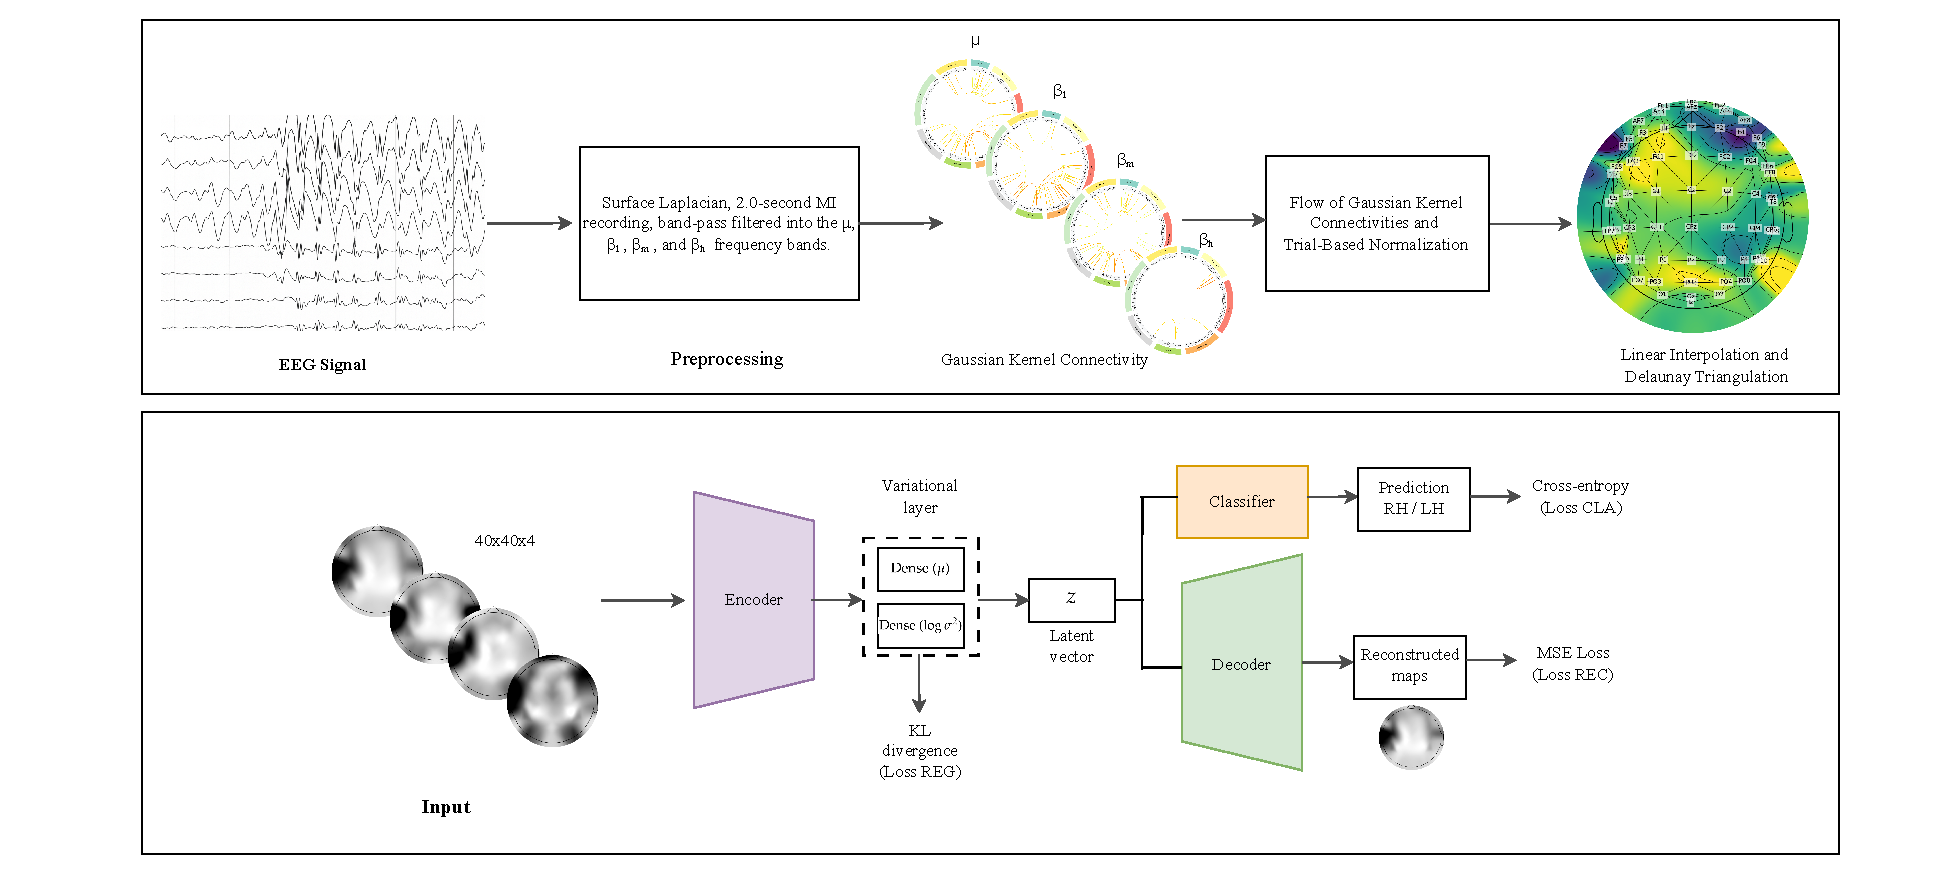
\includegraphics[width=\linewidth]{Figures/Scheme EEG-CIRNET.pdf}
    \caption{The
 proposed \gls{eeggcirnet} framework, composed of two main stages: (\textbf{Top}): A feature engineering pipeline that transforms raw \gls{eeg} signals into multi-channel topographic maps using GFC. {(\textbf{Bottom}):} A VAE architecture that processes these maps to jointly learn reconstruction, classification, and regularization from a shared latent space.}
    \label{fig:EEGCIRNET}
\end{figure}
%------------------------------------------------

% first preprocessing
\subsubsection{Stage 1: Signal Preprocessing and Feature Engineering}

First, an average reference was applied, which included the original reference electrode to ensure the data retained full rank. Subsequently, a fifth-order Butterworth bandpass filter was applied in the 4--40 Hz range. {To reduce computational load and maintain consistency across the evaluated deep learning models, the filtered signals of GigaScience and \gls{eegmmidb} dataset were resampled from 512 Hz and 160 Hz to 128 Hz, respectively~\cite{diagnostics13061122, computers12070145}. This study evaluates the proposed framework on two distinct experimental scenarios. First, for the GigaScience dataset, we focus on the binary classification of Left Hand versus Right Hand \gls{mi} ($Q=2$). This analysis was conducted on a subset of 50 subjects from the original cohort, with participants 29 and 34 excluded due to data availability constraints. Second, for the \gls{eegmmidb} database, the task is extended to the multi-class classification of five interpretable MI categories ($Q=5$). To ensure rigorous experimental consistency and following the experimental setup suggested in~\cite{bouchane2025hybrid}, a specific subset of ten subjects \{3, 7, 8, 9, 12, 13, 40, 41, 49, 50\} was selected, incorporating all valid trials associated with the target classes for these participants.}

Building upon this preprocessed data, the feature engineering process involves applying a Surface Laplacian filter to enhance the spatial resolution of the signals. {Specifically, the temporal segmentation was adapted to the recording protocol of each dataset. For the GigaScience repository, the data was segmented to isolate the active MI period, retaining the window from $2.5$ to $4.5$ s. In contrast, for the \gls{eegmmidb} collection, the entire trial duration of $4.1$ s was utilized.} The segmented data is further decomposed via band-pass filtering into four functionally distinct frequency bands: $\mu$ (8--12 Hz), low-beta ($\beta_l$, \mbox{12--15 Hz}), mid-beta ($\beta_m$, 15--20 Hz), and high-beta ($\beta_h$, 18--40 Hz). For each frequency band, GFC is computed to quantify the functional relationships between all channel pairs. The length scale hyperparameter $\sigma \in \mathbb{R}^+$, ruling the variance of the described data is adjusted to their median estimate as performed in~\cite{alvarez2014unsupervised}. The resulting connectivity information is then condensed into a normalized, channel-wise flow vector for each band. 

\subsubsection{Stage 2: Topographic Map Generation}

The second stage of the pipeline transforms the one-dimensional, GFC-based flow vectors into a two-dimensional, image-based representation suitable for processing with a CNN. This conversion is critical as it re-introduces the spatial topography of the \gls{eeg}electrodes, allowing the model to learn spatially coherent features.

This transformation was achieved via spatial interpolation, a process implemented using the visualization utilities within the MNE-Python library
 (\url{https://mne.tools/stable/index.html}, accessed on 1 June 2025). For each frequency band, the corresponding flow vector's values are mapped to the $2D$ coordinates of the \gls{eeg}electrodes. A mesh is then constructed over these coordinates using Delaunay triangulation. The pixel values for the final topographic map are subsequently estimated using linear barycentric interpolation within this mesh. This procedure is repeated for each of the four frequency bands ($\mu$, $\beta_l$, $\beta_m$, and $\beta_h$), yielding a set of four distinct topographic maps per trial. These maps are then stacked along the channel dimension to form a single, multi-channel image of size $40 \times 40 \times 4$. This resulting data structure serves as the final input to the \gls{eeggcirnet} architecture, providing a rich, spatio-spectral representation of the brain's functional connectivity during \gls{mi}.

\subsubsection{Stage 3: \gls{eeggcirnet} Architecture and Training}

%------------------------------------------
\begin{table}[H]%[h!]
\centering
\caption{Layer-wise configuration of the \gls{eeggcirnet} architecture. The input shape corresponds to the four-channel topographic maps ($\tilde{H} \times \tilde{W} \times C$).}
\label{tab:architecture}
\resizebox{\textwidth}{!}{%
\begin{tabular}{@{}llcccc@{}}
\toprule
\textbf{Block} & \textbf{Layer} & \textbf{Kernel/Units} & \textbf{Strides} & \textbf{Activation} & \textbf{Output Shape} \\ \midrule
\multicolumn{6}{c}{\textbf{Input Image}} \\
& & & & & $(40, 40, 4)$ \\ \midrule
\textbf{Encoder} & Conv2D & $3 \times 3$, 6 Filters & $(1, 1)$ & SELU & $(40, 40, 6)$ \\
($E_{\phi}$) & AvgPool2D & $2 \times 2$ & $(2, 2)$ & - & $(20, 20, 6)$ \\
& Conv2D & $3 \times 3$, 16 Filters & $(1, 1)$ & SELU & $(20, 20, 16)$ \\
& AvgPool2D & $2 \times 2$ & $(2, 2)$ & - & $(10, 10, 16)$ \\
& Conv2D & $3 \times 3$, 120 Filters & $(1, 1)$ & SELU & $(10, 10, 120)$ \\
& Flatten & - & - & - & $(12000)$ \\
& Dense & 128 Units & - & SELU & $(128)$ \\ \midrule
\textbf{Latent Space} & Dense ($\mu$) & 128 Units & - & Linear & $(128)$ \\
(Reparameterization) & Dense ($\log\sigma^2$) & 128 Units & - & Linear & $(128)$ \\ \midrule
\textbf{Decoder} & Dense & 128 Units & - & SELU & $(128)$ \\
($D_{\theta}$) & Dense & 12000 Units & - & SELU & $(12000)$ \\
& Reshape & $(10, 10, 120)$ & - & - & $(10, 10, 120)$ \\
& Conv2DTranspose & $3 \times 3$, 16 Filters & $(1, 1)$ & SELU & $(10, 10, 16)$ \\
& Upsampling & $2 \times 2$ & $(2, 2)$ & - & $(20, 20, 16)$ \\
& Conv2DTranspose & $3 \times 3$, 6 Filters & $(1, 1)$ & SELU & $(20, 20, 6)$ \\
& Upsampling & $2 \times 2$ & $(2, 2)$ & - & $(40, 40, 6)$ \\
& Reconstruction & $3 \times 3$ & - & Sigmoid & $(40, 40, 4)$ \\\midrule
\textbf{Classifier} & Dense & 128 Units & - & SELU & $(128)$ \\
($C_{\psi}$) & Dense (Output) & 2 Units & - & Softmax & $(2)$ \\ \bottomrule
\end{tabular}%
}
\end{table}
%------------------------------------------

The core of this model is a VAE with a convolutional architecture inspired by LeNet-5. This architecture is composed of three interconnected functional blocks operating on a shared latent space: an encoder, a decoder, and a classifier. 

The encoder block consists of two sequential pairs of convolutional and average pooling layers, which extract hierarchical spatial features from the input image. These features are then flattened and passed through a dense layer to produce a compact representation, which in turn parameterizes the mean ($\mu$) and log-variance ($\log\sigma^2$) vectors of the latent space. The decoder mirrors this structure using transposed convolutional layers to upsample the latent representation back to the original image dimensions. Concurrently, the classifier, a simple multi-layer perceptron, operates on the same latent vector to perform the final classification. The detailed layer-wise configuration of the \gls{eeggcirnet} is summarized in Table~\ref{tab:architecture}.

The \gls{eeggcirnet} model was trained end-to-end by optimizing the composite loss function described in Section~\ref{subsec:model}. The training was performed using the Adam optimizer with an initial learning rate of $1 \times 10^{-3}$. The hyperparameters that weight the loss components (i.e., $\lambda_{\text{REC}}$, $\lambda_{\text{CLA}}$, and $\lambda_{\text{REG}}$) were set using
 \texttt{KerasTuner} framework to ensure a balanced contribution from reconstruction, classification, and regularization objectives during training, subject to the constraint that they sum to one. The model was trained for a total of $200$ epochs with a batch size of $64$. An early stopping mechanism was employed with a patience of $10$ epochs, monitoring the validation loss to prevent overfitting and save the model with the best generalization performance. The model performance was evaluated using a subject-specific validation strategy. {For each of the considered subjects, we employed a \textit{Stratified} Shuffle Split
  cross-validation scheme with $5$ repetitions (\texttt{n\_splits=5}).} In each iteration, the trials were randomly partitioned into $80\%$ for training and $20\%$ for testing (\texttt{test\_size=0.2}), ensuring that the class distribution remained balanced in both sets. The results reported in this study correspond to the average accuracy obtained strictly on the {test sets} across these $5$ splits, ensuring that the reported metrics reflect the model's generalization capability on unseen data.

\section{Materials and Methods}

\subsubsection{Laplacian Filtering and Time Segmentation}\label{sec:laplacian}
% Laplacian filter
Each MI trial is structured for the proposed framework. Let $\{\mathbf{X} \in \mathbb{R}^{C \times \tau},\, \mathbf{y} \in \{0,1\}^Q\}$ denote a multichannel \gls{eeg}and its associated MI target label, where $\mathbf{X}$ represents the \gls{eeg} recording with $C$ spatial channels and $\tau$ temporal samples, and $\mathbf{y}$ is a one-hot encoded vector indicating the MI class among $Q$ possible categories.

To enhance the spatial resolution and mitigate the volume conduction effects inherent in \gls{eeg} recordings, a Surface Laplacian filter is applied to each trial $\mathbf{X} $. This filter acts as a spatial high-pass filter by estimating the second spatial derivative of the scalp potential at each electrode $c \in \mathcal{C}$ with respect to its neighbors $c' \in \mathcal{C}$, where $c \neq c'$. Following the methodology in~\cite{cohen2014analyzing}, this is achieved by using spherical splines to project the electrode positions onto a unit sphere, which allows for the interpolation of scalp potentials via Legendre polynomials. The interaction between any pair of electrodes $(c, c')$ is modeled as:
\begin{equation}
    p(c,c') = \frac{1}{4\pi} \sum_{n=1}^{N_{max}} \frac{\alpha (2n+1)P_n\left(\text{cosdist}(\mathbf{e}_c, \mathbf{e}_{c'})\right)}{(n(n+1))^{\rho - \alpha}},
    \label{eq:spline_interpolation}
\end{equation}
%
where $P_n$ is the Legendre Polynomial of order $n$, $N_{max}$ is the highest polynomial order considered, $\rho \in \mathbb{R}^{+}$ is a smoothness constant, and $\mathbf{e}_c, \mathbf{e}_{c'} \in \mathbb{R}^3$ are the 3D electrode positions normalized to a unit-radius sphere. The cosine distance is defined as $\text{cosdist}(\mathbf{e}_c, \mathbf{e}_{c'}) = 1 - \|\mathbf{e}_c - \mathbf{e}_{c'}\|_2 / 2$.

The Laplacian-filtered \gls{eeg} data, denoted as $\mathbf{X_L} \in \mathbb{R}^{C \times \tau}$, is subsequently computed using the weighting matrices derived from the spline interpolation:
%
\begin{equation}
    \mathbf{X_L} = \mathbf{H}\left(\mathbf{X}^{\top}\mathbf{G}_{s}^{-1} - \mathbf{X}^{\top}\mathbf{G}_{s}^{-1}\mathbf{1}\mathbf{G}_{s}^{-1}/\mathbf{1}^{\top}\mathbf{G}_{s}^{-1}\mathbf{1}\right)^{\top},
    \label{eq:laplacian_filter}
\end{equation}
%
where $\mathbf{1} \in \mathbb{R}^{C}$ is a column vector of ones, $\mathbf{I} \in \mathbb{R}^{C \times C}$ is the identity matrix, and $\lambda \in [0, 1]$ is a regularization parameter. The matrix $\mathbf{G}_s = \mathbf{G} + \lambda\mathbf{I}$ is a regularized (smoothed) version of $\mathbf{G}$. The weighting matrices $\mathbf{G}, \mathbf{H} \in \mathbb{R}^{C \times C}$ hold the elements derived from Equation~\eqref{eq:spline_interpolation}, with their specific values determined by the parameter $\alpha$ as follows:
%
\begin{equation}
    \alpha = 
    \begin{cases} 
        1, & \text{where } p(c,c') = g(c,c') \\ 
        -1, & \text{where } p(c,c') = h(c,c') 
    \end{cases},
\end{equation}
%
where $g(c,c')$ and $h(c,c')$ are the elements of matrices $\mathbf{G}$ and $\mathbf{H}$, respectively. This filtering step produces a spatially enhanced representation $\mathbf{X_L}$ that serves as input for the subsequent feature extraction stages.

% Time segmentation
Further, to focus the analysis exclusively on the period of active \gls{mi}, the Laplacian-filtered signal $\mathbf{X_L}$ is temporally segmented. The time window corresponding to the MI task, specifically between $t_s$ and $t_e$ seconds of each trial, is retained. Let $t_s$ and $t_e$ be the start and end times of the MI segment, and $f_s$ be the sampling frequency, the segmented signal $\mathbf{X}_{seg} \in \mathbb{R}^{C \times \tau}$ is obtained as:
%
\begin{equation}
    \mathbf{X}_{seg} = \mathbf{X_L}[:, t_s \cdot f_s : t_e \cdot f_s],
    \label{eq:segmentation}
\end{equation}
%
where the slicing notation $[t_s \cdot f_s : t_e \cdot f_s]$ indicates the selection of temporal samples from the start index to the end index. For brevity, this segmented signal will be denoted as $\mathbf{X}$ in the subsequent sections.

\subsubsection{Kernel-Based Cross-Spectral Gaussian Connectivity for \gls{eeg} Imaging}\label{sec:kcs}

%input-output
To model the mutual dependency between \gls{eeg} channels, we consider any two channels \( \mathbf{x}_c, \mathbf{x}_{c'} \in \mathbb{R}^\tau \) from a given trial $\mathbf{X}$ (where $c,c'\in C$). Their mutual dependency can be captured using a stationary kernel \( \kappa : \mathbb{R}^\tau \times \mathbb{R}^\tau \rightarrow \mathbb{R} \), which maps both signals into a reproducing kernel Hilbert space (RKHS) via a nonlinear feature map \( \phi : \mathbb{R}^\tau \rightarrow \mathcal{H} \)~\cite{kanagawa2018gaussianprocesseskernelmethods}. Indeed, according to Bochner’s theorem, a sufficient condition for the kernel $\kappa$ to be stationary is that it admits a spectral representation~\cite{JMLR:v25:22-1434}:
\begin{equation}
\kappa(\mathbf{x}_c - \mathbf{x}_{c'}) = \int_{{\Omega_b}} \exp\left( j2\pi (\mathbf{x}_c - \mathbf{x}_{c'})^\top \mathbf{f} \right) S_{\mathbf{x}_c\mathbf{x}_{c'}}(\mathbf{f})\, d\mathbf{f},
\label{eq:stationary_kernel}
\end{equation}
where \( \mathbf{f} \in \boldsymbol{\Omega} \subseteq \mathbb{R}^\tau \) is a frequency vector, and \( S_{\mathbf{x}_c\mathbf{x}_{c'}}(\mathbf{f}) = \frac{dP_{\mathbf{x}_c\mathbf{x}_{c'}}(\mathbf{f})}{d\mathbf{f}} \in \mathbb{C} \) is the cross-spectral density between \( \mathbf{x} \) and \( \mathbf{x}' \), derived from the spectral distribution \( P_{\mathbf{x}_c\mathbf{x}_{c'}}(\mathbf{f}) \).

Building on this spectral representation, the cross-spectral power within a specific frequency band $\Omega_b$ can be computed via the Fourier transform of the kernel:
\begin{equation}
P_{\mathbf{x}_c\mathbf{x}_{c'}}({\Omega_b}) = 2 \int_{{\Omega_b}} \mathcal{F}\left\{ \kappa(\mathbf{x}_c - \mathbf{x}_{c'}) \right\} d\mathbf{f},
\label{eq:cross_spectral_band}
\end{equation}
where \( \mathcal{F}\{\cdot\} \) denotes the Fourier transform. This spectral formulation allows capturing both linear and nonlinear dependencies in the frequency domain, making it particularly useful for analyzing brain signals.

A widely used choice for \( \kappa \) is the Gaussian kernel, which ensures smoothness, locality, and analytic tractability~\cite{rasmussen2006gaussian}:
\begin{equation}
\kappa_G(\mathbf{x}_c - \mathbf{x}_{c'}; \sigma) = \exp\left( -\frac{\|\mathbf{x}_c - \mathbf{x}_{c'}\|_2^2}{2\sigma^2} \right),
\end{equation}
where \( \sigma \in \mathbb{R}^+ \) is a bandwidth hyper-parameter.

%filter bank
Inspired by the kernel-based spectral approaches introduced in~\cite{diagnostics13061122}, we compute a Gaussian kernel cross-spectral connectivity estimator to encode spatio--frequency interactions among pairwise \gls{eeg} channels. Specifically, for each \gls{eeg} channel \( c \), a band-limited spectral reconstruction is obtained as:
\begin{equation}\label{eq:fbank}
\mathbf{x}_c^{({\Omega_b})} = 
\mathcal{F}^{-1}\left\{\mathcal{F}\{\mathbf{x}_c\}; {\Omega_b}\right\},
\end{equation}
where \( {\Omega_b} \) denotes a given frequency bandwidth (rhythm). 
Then, the Gaussian Function Connectivity (GFC) matrix 
\( \mathbf{K}^{({\Omega_b})} \in [0,1]^{C\times C} \) is derived to quantify 
the degree of similarity between the spectral representations of all channel pairs, as:
\begin{equation}
K^{({\Omega_b})}_{cc'} = 
\kappa_G\left(\mathbf{x}^{({\Omega_b})}_c - \mathbf{x}^{({\Omega_b})}_{c'}; 
\sigma_{{\Omega_b}}\right),
\label{eq:gfc}
\end{equation}
where \( \kappa_G(\cdot; \sigma_{{\Omega_b}}) \) is a Gaussian kernel with scale parameter \( \sigma_{{\Omega_b}} \). To ensure adaptive sensitivity across rhythms, \( \sigma_{{\Omega_b}} \) is estimated as the 
median of all pairwise Euclidean distances between spectral reconstructions 
\( \mathbf{x}^{({\Omega_b})}_c \) and \( \mathbf{x}^{({\Omega_b})}_{c'} \), \( \forall\, c,c'\in C \). This formulation provides a data-driven normalization of connectivity strength, enabling robust comparison across heterogeneous \gls{eeg} rhythms and subjects.

%GFC flow
Afterward, we propose to compute an \gls{eeg} connectivity flow from 
\(\mathbf{K}^{({\Omega_b})}\), preserving a direct one-to-one correspondence 
with the electrode spatial configuration. Specifically, the GFC flow vector \(\mathbf{g}^{({\Omega_b})} \in [0,1]^C\) holds elements:
\begin{equation}\label{eq:flowGFC}
g_c^{({\Omega_b})} = 
\frac{1}{C} \sum_{\substack{c'=1 \\ c' \neq c}}^{C} 
K^{({\Omega_b})}_{cc'},
\end{equation}
where each element \( g_c^{({\Omega_b})} \) represents the mean functional coupling of channel \( c \) with all other channels within the given frequency band \({\Omega_b} \). The latter compresses the pairwise connectivity information into a compact, channel-wise flow representation while retaining the spatial and spectral data patterns.

To ensure a consistent feature scale for the imaging stage, the GFC flow vectors are normalized across the entire training dataset. Specifically, a channel-wise Min-Max normalization is applied, scaling the connectivity values of each channel to a uniform range of $[0, 1]$. This procedure preserves the relative topography of neural connectivity while standardizing the input scale, yielding the normalized flow vector $\tilde{\mathbf{g}}^{(\Omega_b)}$ for each trial.

\subsubsection{Topographic Map Generation}

%topographic interpolation
The final feature engineering step transforms the one-dimensional GFC flow vectors into two-dimensional topographic images, creating a data representation suitable for convolutional neural network (CNN) architectures. For each trial, this process converts the normalized flow vector $\tilde{\mathbf{g}}^{(\Omega_b)} \in [0, 1]^C$ from each frequency band into a corresponding topographic image $\mathbf{T}^{(\Omega_b)} \in \mathbb{R}^{\tilde{H} \times \tilde{W}}$.

This transformation is accomplished via spatial interpolation guided by Delaunay triangulation. First, the set of 2D scalp coordinates of the electrodes, $P = \{(x_c, y_c)\}_{c=1}^C$, is triangulated. This partitions the electrode layout into a mesh of non-overlapping triangles, where the circumcircle of each triangle contains no other electrode points. This triangulation provides a structured grid for interpolating the connectivity values, where each element $\tilde{g}_c^{(\Omega_b)}$ is associated with its corresponding coordinate $(x_c, y_c)$.

To generate the final image, the value $V(x, y)$ for each pixel is computed using barycentric interpolation within its enclosing triangle $T_k = (p_1, p_2, p_3)$:
%
\begin{equation}
    V(x, y) = \lambda_1(x, y) v(p_1) + \lambda_2(x, y) v(p_2) + \lambda_3(x, y) v(p_3),
    \label{eq:barycentric_interpolation}
\end{equation}
%
where $v(p_i)$ is the connectivity value at vertex $p_i$, and $\lambda_1, \lambda_2, \lambda_3$ are the barycentric coordinates of $(x, y)$ satisfying $\sum_{j=1}^{3} \lambda_j = 1$ and $\lambda_j \geq 0$. This procedure is applied across all pixels to render the smooth topographic map $\mathbf{T}^{(\Omega_b)}$. The resulting set of four maps (one for each frequency band) is then stacked to form a multi-channel image, which serves as the final input to the deep learning model.


\subsubsection{\gls{eeggcirnet}: Multimodal Architecture}\label{subsec:model}

The proposed model is a variational autoencoder (VAE) designed to process topographic maps derived from functional connectivity representations. Its architecture relies on a single input stream that learns to extract and encode the most relevant spatial features from the maps, which are then projected into a shared latent space where a multivariate Gaussian distribution is modeled. From this latent space, the model simultaneously performs reconstruction of the topographic maps and classification of \gls{mi} tasks. These objectives are integrated within a composite loss function that balances reconstruction fidelity, classification accuracy, and latent space regularization. This approach enables the learning of robust and interpretable latent representations capable of capturing discriminative spatial relationships and adapting to the variability and noise inherent in \mbox{\gls{eeg} signals.}

The core of our framework is a VAE based on the LeNet-5 architecture, which is partitioned into three functional blocks: an encoder, a decoder, and a classifier, all operating on the shared latent space. Let $Y \in \mathbb{R}^{\tilde{H} \times \tilde{W} \times B}$ be the multi-channel input image for a given trial, formed by stacking the $B$ topographic maps (one for each frequency band).

The encoder, defined as a function $E_{\phi}$ parameterized by $\phi$, maps the input image $Y$ to the parameters of the posterior distribution $q_{\phi}(z|Y)$. This transformation is realized through a composition of functions, where each function represents a layer in the network:
\begin{equation}
    h_E = (f_5 \circ f_4 \circ f_3 \circ f_2 \circ f_1)(Y)
\end{equation}

Here, $f_1$ and $f_3$ are convolutional layers with {SELU} activation, $f_2$ and $f_4$ are average pooling layers, and $f_5$ is a fully connected layer with {SELU} activation after flattening the feature maps. The resulting hidden representation $h_E$ is then linearly transformed to produce the mean vector $\mu$ and the log-variance vector $\log \sigma^2$ of the latent space:
\begin{align}
    \mu &= W_{\mu}h_E + b_{\mu} \\
    \log \sigma^2 &= W_{\sigma}h_E + b_{\sigma}
\end{align}

The decoder, defined as a function $D_{\theta}$ parameterized by $\theta$, reconstructs the original input image $\hat{Y}$ from a latent vector $z \sim q_{\phi}(z|Y)$. Its architecture mirrors the encoder by composing functions that progressively up-sample the representation to the original \mbox{image dimensions:}
\begin{equation}
    \hat{Y} = (g_3 \circ g_2 \circ g_1)(z)
\end{equation}

Here,
$g_1$ is a fully connected layer followed by a reshape operation, $g_2$ is a transposed convolutional layer with {SELU} activation, and $g_3$ is a final transposed convolutional layer with a Sigmoid activation to ensure the output pixel values are in a normalized range.

Concurrently, the classifier, a function $C_{\psi}$ parameterized by $\psi$, predicts the MI task label probabilities $\hat{p}$ from the same latent vector $z$. It is implemented as a multi-layer perceptron:
\begin{equation}
    \hat{p} = C_{\psi}(z) = \text{Softmax}(W_c( \text{SELU}(W_h z + b_h)) + b_c)
\end{equation}

Formally, the latent vector $z_i$ for a given input sample $i$ is computed using the reparameterization trick:
\begin{equation}
    z_i = \mu_i + \exp\left(\frac{1}{2}\log\sigma_i^2\right) \odot \epsilon_i, \quad \epsilon_i \sim \mathcal{N}(0, I)
\end{equation}
where $\mu_i$ and $\sigma_i^2$ denote the mean and variance of the approximate posterior distribution learned by the encoder for sample $i$, and $\epsilon_i$ is drawn from a standard normal distribution. The exponential term ensures the sampled standard deviation remains strictly positive.

The total objective function, $\mathcal{L}_{\text{total}}$, is defined as a weighted sum of the three loss terms:
\begin{align}
\mathcal{L}_{\text{total}} = \ & \lambda_{\text{REC}} \cdot \mathcal{L}_{\text{REC}} + \lambda_{\text{CLA}} \cdot \mathcal{L}_{\text{CLA}} + \lambda_{\text{REG}} \cdot \mathcal{L}_{\text{REG}} \\
\intertext{where}
\mathcal{L}_{\text{REC}} &= \frac{ \frac{1}{N} \sum_{i=1}^{N} \lVert Y_i - \hat{Y}_i \rVert_F^2 }{ \frac{1}{N} \sum_{i=1}^{N} \lVert Y_i - \bar{Y} \rVert_F^2 } \label{eq:rec} \\
\mathcal{L}_{\text{CLA}} &= \frac{1}{N} \sum_{i=1}^{N} \frac{ \mathcal{L}_{\mathrm{cce}}(p_i, \hat{p}_i) }{ \mathcal{L}_{\mathrm{cce}}([0.5, 0.5], \hat{p}_i)} \label{eq:cla} \\
\mathcal{L}_{\text{REG}} &= \frac{1}{N \log N} \sum_{i=1}^{N} D_{\text{KL}}(q_{\phi}(z_i|Y_i) || \mathcal{N}(0, I)) \label{eq:reg}
\end{align}

\noindent
where $\lambda_{\text{REC}}$, $\lambda_{\text{CLA}}$, and $\lambda_{\text{REG}}$ are hyperparameters controlling the contribution of each term.
The first component, $\mathcal{L}_{\text{REC}}$, is the normalized mean squared error (NMSE), which evaluates reconstruction accuracy by comparing the original topographic maps ($Y_i$) and their reconstructions ($\hat{Y}_i$), normalized by the dataset's variance ($\bar{Y}$ is the mean image). The Frobenius norm, $\lVert \cdot \rVert_F$, is used for the image-wise error.
The second term, $\mathcal{L}_{\text{CLA}}$, represents the normalized binary cross-entropy (NBCE). It penalizes misclassifications between the true one-hot labels ($p_i$) and predicted probabilities ($\hat{p}_i$), while adjusting the loss based on the entropy over an ideal, non-informative prediction (e.g., a uniform distribution $[0.5, 0.5]$). This maintains a balanced contribution from all classes.
Finally, the third term, $\mathcal{L}_{\text{REG}}$, is the normalized Kullback–Leibler (KL) divergence between the approximate posterior $q_{\phi}(z_i|Y_i)$ and a unit Gaussian prior $\mathcal{N}(0, I)$. This regularizes the latent space, promoting smoothness and disentanglement in the learned representations.

This KL divergence term encourages the latent representations to follow a standard normal distribution, promoting structure and generalization. The use of $\log N$ in the denominator prevents this term from dominating the loss in large batches. Taken together, these components ensure that the model jointly optimizes for faithful reconstruction, discriminative performance, and a well-regularized latent structure—crucial for interpretable and generalizable multimodal brain–computer interfaces.

The model is trained by solving the following optimization problem:
\[
\{\phi^*, \theta^*, \psi^*\} = \arg\min_{\phi, \theta, \psi} \mathcal{L}_{\text{total}}
\]
where $\{\phi, \theta, \psi\}$ denotes the complete set of trainable parameters in the encoder, decoder, and classifier, respectively.



\subsubsection{Evaluation Criteria}

The performance of the proposed \gls{eeggcirnet} was rigorously evaluated using a multi-faceted approach tailored to the specific requirements of each experimental scenario. For the GigaScience dataset ($Q=2$), the primary quantitative metric was subject-specific binary classification accuracy, benchmarked against seven baseline and state-of-the-art models. For the \gls{eegmmidb} dataset, the evaluation was extended to a multi-class setting ($Q=5$), focusing on the model's ability to resolve complex decision boundaries across five distinct \gls{mi} categories.

To validate the findings, a robust statistical framework was employed. A Friedman test was used to assess overall significance across models, followed by post-hoc pairwise $t$-tests for direct comparisons. To account for the multiple comparisons problem, the resulting $p$-values were adjusted using the \textit{Holm-Bonferroni} correction method to control the family-wise error rate. Furthermore, the framework's robustness and generalization capabilities were analyzed by stratifying the GigaScience cohort into ``Good'' (accuracy $> 80\%$), ``Mid'' (accuracy $60\%$--$80\%$), and ``Bad'' (accuracy $< 60\%$) performance groups based on the standard EEGNet baseline. This stratification allowed for a targeted assessment of the model's corrective effectiveness across varying \gls{eeg}signal qualities.

Beyond quantitative metrics, the evaluation delved into the model's interpretability by leveraging its variational autoencoder architecture and gradient-based analysis. This qualitative assessment involved three key methods: \textit{(i)} a visual analysis of the reconstructed topographic maps to confirm that the model learned physiologically relevant spatio-spectral patterns; \textit{(ii)} the visualization of the latent space using t-SNE projections to directly inspect the quality of class separability and feature disentanglement; and \textit{(iii)}~a layer-wise relevance analysis using Grad-CAM++. The latter was employed to verify that the model's decision-making is driven by spatial contributions from neurophysiologically valid regions---such as the sensorimotor cortex---rather than artifacts. This combined quantitative and qualitative evaluation provides a holistic validation of the \gls{eeggcirnet} framework, covering its accuracy, statistical significance, and the meaningfulness of its learned internal representations.

\subsection{Results}\label{sec:Results}
%------------------------------------------------

\subsubsection{Binary MI Classification Performance on the GigaScience Database}
%------------------------------------------------
\begin{figure}[H]
  %----- PALETA (Tableau-like)
\definecolor{modelBlue}{RGB}{31,119,180}   % EEGNet
\definecolor{modelOrange}{RGB}{255,127,14} % KREEGNet
\definecolor{modelGreen}{RGB}{44,160,44}   % KCS-FCNet
\definecolor{modelRed}{RGB}{214,39,40}     % DeepConvNet
\definecolor{modelPurple}{RGB}{148,103,189}% ShallowConvNet
\definecolor{modelBrown}{RGB}{140,86,75}   % TCFusionNet
\definecolor{modelGray}{RGB}{127,127,127}  % CSP
\definecolor{modelOlive}{RGB}{188,189,34}  % \gls{eeggcirnet} (NRVAE)

%----- ESTILOS (sin markers globalmente)
\pgfplotsset{
  every axis plot/.style={solid, mark=none}, % <-- sin marcadores
  myaxis/.style={
    width=0.9\linewidth,
    height=0.16\paperheight,
    scale only axis,
    ymin=0.40, ymax=1.00,
    xtick pos=bottom,
    ytick pos=left,
    tick align=inside,
    ytick={0.40,0.50,0.60,0.70,0.80,0.90,1.00},
    yticklabels={40,50,60,70,80,90,100},
    ylabel={Accuracy (\%)},
    xlabel={Subjects},
    xmin=-0.5, xmax=49.5,   % datos x = 0..49
    xtick=data,
    xticklabel style={rotate=90, anchor=east, font=\scriptsize},
    yticklabel style={font=\scriptsize},
    label style={font=\small},
    axis lines=box,
    xmajorgrids, ymajorgrids,
    grid style={black!15},
    legend style={
  at={(0.004,0.35)}, anchor=north west, % esquina sup. izquierda del recuadro de la gráfica
  draw=black!25, fill=white, fill opacity=0.8, text opacity=1,
  font=\scriptsize,                
  inner sep=0.4pt,            
  row sep=0.4pt, column sep=1pt 
},
legend image post style={xscale=0.3},
legend cell align=left,
legend columns=2, 
  }
}

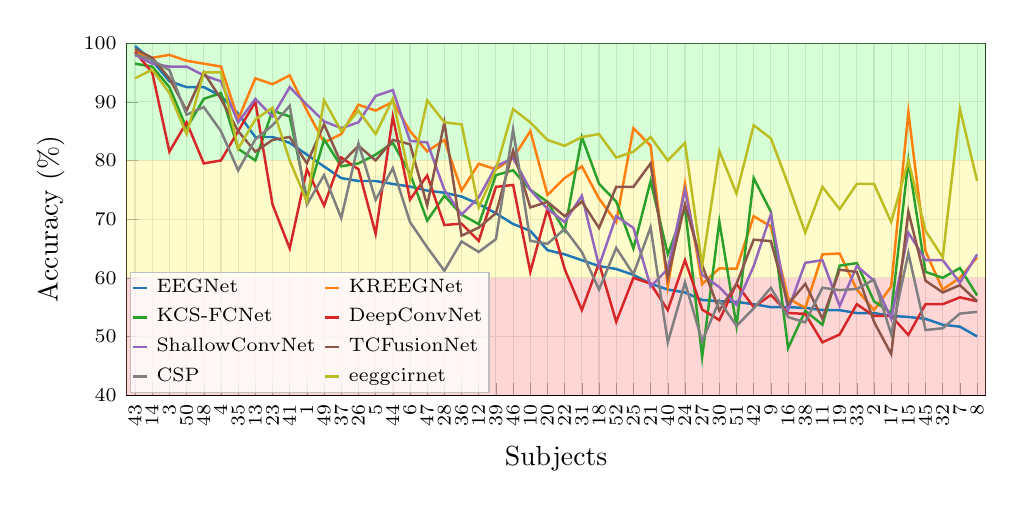
\begin{tikzpicture}
\begin{axis}[myaxis,
  xticklabels={43,14,3,50,48,4,35,13,23,41,1,49,37,26,5,44,6,47,28,36,12,39,46,10,20,22,31,18,52,25,21,40,24,27,30,51,42,9,16,38,11,19,33,2,17,15,45,32,7,8}
]

  %----- Bandas de fondo (0.40–0.60 rojo, 0.60–0.80 amarillo, 0.80–1.00 verde)
  \path[fill=red!40,    opacity=0.40] (axis cs:-0.5,0.40) rectangle (axis cs:49.5,0.60);
  \path[fill=yellow!50, opacity=0.40] (axis cs:-0.5,0.60) rectangle (axis cs:49.5,0.80);
  \path[fill=green!40,  opacity=0.40] (axis cs:-0.5,0.80) rectangle (axis cs:49.5,1.00);

  %----- Curvas (sin markers)
  \addplot[line width=0.9pt, color=modelBlue]
     coordinates {(0,0.99500) (1,0.97000) (2,0.93500) (3,0.92500) (4,0.92500) (5,0.91000) (6,0.88000) (7,0.84000) (8,0.84000) (9,0.83000) (10,0.81000) (11,0.78970) (12,0.77000) (13,0.76500) (14,0.76500) (15,0.76000) (16,0.75560) (17,0.74870) (18,0.74500) (19,0.73850) (20,0.72570) (21,0.71000) (22,0.69170) (23,0.68000) (24,0.64710) (25,0.64000) (26,0.63000) (27,0.62000) (28,0.61500) (29,0.60500) (30,0.59000) (31,0.58000) (32,0.57500) (33,0.56220) (34,0.56000) (35,0.55900) (36,0.55500) (37,0.55000) (38,0.55000) (39,0.54870) (40,0.54500) (41,0.54480) (42,0.54000) (43,0.54000) (44,0.53500) (45,0.53330) (46,0.53000) (47,0.52000) (48,0.51670) (49,0.50000)};
  \addlegendentry{EEGNet}

  \addplot[line width=0.9pt, color=modelOrange]
    coordinates {(0,0.98500) (1,0.97500) (2,0.98000) (3,0.97000) (4,0.96500) (5,0.96000) (6,0.87000) (7,0.94000) (8,0.93000) (9,0.94500) (10,0.88500) (11,0.83080) (12,0.84500) (13,0.89500) (14,0.88500) (15,0.90000) (16,0.85000) (17,0.81540) (18,0.83500) (19,0.74870) (20,0.79430) (21,0.78500) (22,0.80420) (23,0.85000) (24,0.74120) (25,0.77000) (26,0.79000) (27,0.73500) (28,0.69500) (29,0.85500) (30,0.82500) (31,0.58500) (32,0.76000) (33,0.58920) (34,0.61600) (35,0.61540) (36,0.70500) (37,0.68750) (38,0.56500) (39,0.54870) (40,0.64000) (41,0.64140) (42,0.58000) (43,0.54500) (44,0.58500) (45,0.88210) (46,0.64500) (47,0.58000) (48,0.60000) (49,0.63500)};
  \addlegendentry{KREEGNet}

  \addplot[line width=0.9pt, color=modelGreen]
    coordinates {(0,0.96500) (1,0.96000) (2,0.92500) (3,0.85500) (4,0.90500) (5,0.91500) (6,0.82000) (7,0.80000) (8,0.88500) (9,0.87500) (10,0.73500) (11,0.83590) (12,0.79000) (13,0.79500) (14,0.81000) (15,0.83000) (16,0.77780) (17,0.69740) (18,0.74000) (19,0.70770) (20,0.69140) (21,0.77500) (22,0.78330) (23,0.75000) (24,0.72940) (25,0.68000) (26,0.84000) (27,0.76000) (28,0.73000) (29,0.65000) (30,0.76500) (31,0.64000) (32,0.72000) (33,0.46490) (34,0.69600) (35,0.51790) (36,0.77000) (37,0.71250) (38,0.48000) (39,0.54360) (40,0.52000) (41,0.62070) (42,0.62500) (43,0.56000) (44,0.54000) (45,0.80000) (46,0.61000) (47,0.60000) (48,0.61670) (49,0.57000)};
  \addlegendentry{KCS-FCNet}

  \addplot[line width=0.9pt, color=modelRed]
    coordinates {(0,0.98500) (1,0.95000) (2,0.81500) (3,0.86500) (4,0.79500) (5,0.80000) (6,0.85000) (7,0.90000) (8,0.72500) (9,0.65000) (10,0.78500) (11,0.72310) (12,0.80500) (13,0.78500) (14,0.67500) (15,0.87500) (16,0.73330) (17,0.77440) (18,0.69000) (19,0.69230) (20,0.66290) (21,0.75500) (22,0.75830) (23,0.61000) (24,0.71760) (25,0.61500) (26,0.54500) (27,0.62500) (28,0.52500) (29,0.60000) (30,0.59000) (31,0.54500) (32,0.63000) (33,0.54590) (34,0.52800) (35,0.58970) (36,0.55000) (37,0.57080) (38,0.54000) (39,0.53850) (40,0.49000) (41,0.50340) (42,0.55500) (43,0.53500) (44,0.53500) (45,0.50260) (46,0.55500) (47,0.55500) (48,0.56670) (49,0.56000)};
  \addlegendentry{DeepConvNet}

  \addplot[line width=0.9pt, color=modelPurple]
    coordinates {(0,0.98000) (1,0.96500) (2,0.96000) (3,0.96000) (4,0.94500) (5,0.93500) (6,0.86500) (7,0.90500) (8,0.87500) (9,0.92500) (10,0.89500) (11,0.86670) (12,0.85500) (13,0.86500) (14,0.91000) (15,0.92000) (16,0.83330) (17,0.83080) (18,0.75000) (19,0.70770) (20,0.73710) (21,0.79000) (22,0.80420) (23,0.75000) (24,0.71760) (25,0.69500) (26,0.74000) (27,0.62000) (28,0.70500) (29,0.68500) (30,0.58500) (31,0.61500) (32,0.75000) (33,0.60540) (34,0.58400) (35,0.55380) (36,0.62000) (37,0.70830) (38,0.54500) (39,0.62560) (40,0.63000) (41,0.55170) (42,0.62000) (43,0.59500) (44,0.53000) (45,0.67690) (46,0.63000) (47,0.63000) (48,0.59170) (49,0.64000)};
  \addlegendentry{ShallowConvNet}

  \addplot[line width=0.9pt, color=modelBrown]
    coordinates {(0,0.99000) (1,0.97500) (2,0.94000) (3,0.88500) (4,0.95000) (5,0.90500) (6,0.85000) (7,0.81500) (8,0.83500) (9,0.84000) (10,0.79500) (11,0.86150) (12,0.79500) (13,0.82500) (14,0.80000) (15,0.83500) (16,0.82780) (17,0.72310) (18,0.86500) (19,0.67180) (20,0.68570) (21,0.71000) (22,0.81670) (23,0.72000) (24,0.72940) (25,0.70500) (26,0.73000) (27,0.68500) (28,0.75500) (29,0.75500) (30,0.79500) (31,0.60000) (32,0.72500) (33,0.62160) (34,0.54400) (35,0.58970) (36,0.66500) (37,0.66250) (38,0.55500) (39,0.58970) (40,0.53000) (41,0.61380) (42,0.61000) (43,0.52500) (44,0.47000) (45,0.71280) (46,0.59500) (47,0.57500) (48,0.58750) (49,0.56000)};
  \addlegendentry{TCFusionNet}

  \addplot[line width=0.9pt, color=modelGray]
     coordinates {(0,0.98100) (1,0.97100) (2,0.95400) (3,0.87800) (4,0.89100) (5,0.85000) (6,0.78300) (7,0.83600) (8,0.86000) (9,0.89300) (10,0.72500) (11,0.77500) (12,0.70200) (13,0.82900) (14,0.73300) (15,0.78700) (16,0.69500) (17,0.65200) (18,0.61200) (19,0.66200) (20,0.64400) (21,0.66600) (22,0.85300) (23,0.66300) (24,0.65800) (25,0.68300) (26,0.64400) (27,0.58000) (28,0.65100) (29,0.60600) (30,0.68600) (31,0.49000) (32,0.59200) (33,0.49200) (34,0.56100) (35,0.51800) (36,0.54800) (37,0.58300) (38,0.53300) (39,0.52400) (40,0.58300) (41,0.57900) (42,0.58100) (43,0.59700) (44,0.50400) (45,0.64200) (46,0.51100) (47,0.51400) (48,0.53900) (49,0.54200)};
  \addlegendentry{CSP}

  \addplot[line width=0.9pt, color=modelOlive]
    coordinates {(0,0.94000) (1,0.95490) (2,0.91500) (3,0.84500) (4,0.95000) (5,0.95000) (6,0.82000) (7,0.86990) (8,0.89000) (9,0.80000) (10,0.73000) (11,0.90250) (12,0.85000) (13,0.88500) (14,0.84500) (15,0.90500) (16,0.76700) (17,0.90250) (18,0.86500) (19,0.86150) (20,0.72000) (21,0.78490) (22,0.88750) (23,0.86490) (24,0.83500) (25,0.82500) (26,0.84000) (27,0.84500) (28,0.80490) (29,0.81500) (30,0.84000) (31,0.80000) (32,0.83000) (33,0.62100) (34,0.81600) (35,0.74350) (36,0.86000) (37,0.83750) (38,0.75990) (39,0.67690) (40,0.75500) (41,0.71700) (42,0.76000) (43,0.76000) (44,0.69500) (45,0.80000) (46,0.67990) (47,0.63500) (48,0.88800) (49,0.76500)};
  \addlegendentry{\gls{eeggcirnet}}

\end{axis}
\end{tikzpicture}
      \caption{Inter-subject accuracy results. Subjects are sorted based on EEGNet performance.The background colors indicate subject performance groups: 
red corresponds to the ``Bad'' group (accuracy $\leq$ 60\%), 
yellow to the ``Mid'' group (60\% $<$ accuracy $\leq$ 80\%), 
and green to the ``Good'' group (accuracy $>$ 80\%).}
   \label{fig:accuracies_models_8}
\end{figure}
%------------------------------------------------
To evaluate the model's robustness against the well-documented challenge of ``BCI illiteracy'', we stratified subjects into performance groups. This stratification was based on the accuracy of EEGNet, a widely-used, state-of-the-art benchmark for EEG-based BCI. This approach allows for a standardized and unbiased assessment of our model's comparative effectiveness, particularly its ability to improve performance for users who struggle with conventional systems. Figure~\ref{fig:accuracies_models_8} illustrates the subject-wise classification performance, where a clear advantage of \gls{eeggcirnet} becomes evident, particularly in challenging cases. Within the ``Bad'' group—comprising subjects with low-quality or highly variable \gls{eeg}signals—conventional models like CSP, ShallowConvNet, and DeepConvNet consistently yield low and unstable results, reflecting their limited ability to handle noise and inter-subject variability. While architectures such as EEGNet and KREEGNet show more stable behavior, their performance remains inconsistent. In stark contrast, \gls{eeggcirnet} entirely eliminates the ``Bad'' performance group, demonstrating a generalized improvement and a notable reduction in inter-subject variability. This outcome strongly suggests that the model’s variational formulation and latent space regularization provide robust feature encoding, effectively preventing the critical performance failures seen in other architectures~\cite{lee2022intertask, mishra2024adversarial}.

\gls{eeggcirnet} extends its advantage into the ``Mid'' group, consistently outperforming competing models like TCFusionNet and KREEGNet across most subjects. This stability under intermediate conditions underscores the model's strong generalization capability, as it delivers reliable performance even with moderately variable \gls{eeg}signals. These results validate the effectiveness of the variational approach in preserving discriminative information while maintaining training stability~\cite{Dhanushkodi}.

In the ``Good'' group, where most architectures achieve high accuracy, \gls{eeggcirnet} performs competitively, matching or exceeding the results of TCFusionNet, KREEGNet, and EEGNet. Critically, its performance is marked by greater consistency across subjects, highlighting its ability to maintain high accuracy without overfitting. This behavior contrasts sharply with deeper architectures like DeepConvNet, which are more susceptible to performance degradation in subject-specific tasks~\cite{electronics12122743}.

Collectively, the subject-wise results in Figure~\ref{fig:accuracies_models_8} underscore that \gls{eeggcirnet} achieves a superior balance of accuracy, stability, and generalization. This positions it as a highly effective and well-rounded model for \gls{eeg}decoding~\cite{app152011150, 11215710}. The aggregate performance metrics summarized in Table~\ref{tab:acc_gain} confirm these subject-wise trends. \gls{eeggcirnet} stands out as the best-performing model overall, achieving the highest average accuracy (\textbf{$81.82\%$}) and the lowest standard deviation ($\pm 10.15$), which confirms its strong generalization and inter-subject stability.

%-----------------------------------------------
\begin{table}[H]%[htbp]
    \centering
    \caption{MI-\gls{eeg} classification performance comparison: Average ACC $\pm$ standard deviation. The standard deviation represents the variability of classification accuracy across the $50$ subjects.}
{
    \begin{tabularx}{\textwidth}{CC}
        \toprule
        \textbf{Model} & \textbf{ACC [\%]} \\
        \midrule
        CSP~\cite{ang2008filter} & $67.66 \pm 13.81$ \\
        EEGNet~\cite{lawhern2018eegnet} & $68.39 \pm 15.50$ \\
        KREEGNet~\cite{tobon2023kreegnet} & $77.32 \pm 14.74$ \\
        KCS-FCNet~\cite{diagnostics13061122} & $72.77 \pm 13.53$ \\
        DeepConvNet~\cite{schirrmeister2017deep} & $66.55 \pm 14.24$ \\
        ShallowConvNet~\cite{Kim2022} & $74.56 \pm 14.60$ \\
        TCFusionNet~\cite{Musallam2021} & $72.81 \pm 14.10$ \\
       \textbf{\gls{eeggcirnet} (Ours)} & $\mathbf{81.82 \pm 10.15}$ \\
        \bottomrule
    \end{tabularx}}
    \label{tab:acc_gain}
\end{table}
%----------------------------------------------

Notably, while KREEGNet achieves a competitive average accuracy ($77.32\%$), its greater performance variability ($\pm 14.74$) indicates reduced stability. Taken together, these results position \gls{eeggcirnet} as the most reliable alternative, outperforming all reference architectures in both classification accuracy and consistency.

{To validate that the observed performance differences among the models were statistically meaningful, a rigorous statistical analysis was conducted. A Friedman test was first applied to the subject-wise accuracies of all eight models, yielding a test statistic with a $p$-value lower than the detection threshold ($p < 0.01$) for proposed \gls{eeggcirnet} model. This result allows for the rejection of the null hypothesis of equal medians with a high level of confidence, confirming that statistically notable differences exist across the \mbox{evaluated architectures.}}

{The nature of these differences is detailed in Figure~\ref{fig:consitency} and Table~\ref{tab:p-values_updated}. The subject-wise ranking heatmap (Figure~\ref{fig:consitency}a) visually confirms the performance tiers, highlighting the consistent top rankings of \gls{eeggcirnet} and KREEGNet, the intermediate performance of models like TCFusionNet and ShallowConvNet, and the instability of DeepConvNet and CSP. The matrix of $p$-values from post-hoc pairwise t-tests (Figure~\ref{fig:consitency}b) further reinforces this, revealing statistical differences between the high- and low-performing models.}

% \vspace{-20pt}
% %-----------------------------------------------
% \begin{figure}[htbp]

%         \raisebox{18pt}{\subfloat[Model rankings based on performance.]{\scalebox{0.60}{\begin{tikzpicture}
% \begin{axis}[
%  width=10.2cm, height=8.2cm,
%   axis lines=box, axis on top, enlargelimits=false,
%   xmin=-0.5, xmax=49.5,
%   ymin=-0.5, ymax=7.5,
%   tick align=inside,
%   xtick pos=bottom,
%   ytick pos=left,
%   ytick={0,...,7},
%   yticklabels={EEGNet,KCS-FCNet,KREEGNet,DeepConvNet,ShallowConvNet,TCFusionNet,CSP,EEG-GCIRNet},
%   xtick={0,10,20,30,40,49},
%   xticklabels={43,1,12,21,11,8},
%   colorbar,
%   colormap={reverse winter}{
%         indices of colormap={
%             \pgfplotscolormaplastindexof{viridis},...,0 of viridis}
%     },
%   colorbar style={
%     width=5mm,
%     ticklabel style={font=\small},
%   },
% ]

% \addplot[
%     matrix plot*,
%     patch type=rectangle,
%     mesh/rows=8,
%     mesh/cols=50,
%     point meta=explicit
%   ]
%   table [x=x, y=y, meta=val, col sep=comma] {ranking_long.csv};
% \end{axis}
% \end{tikzpicture}
% }}} \label{fig:ranking}       
%         \subfloat[\emph{t}-test independence-test \emph{p}-values.]{\scalebox{0.60}{\begin{tikzpicture}
% \begin{axis}[
%   width=8.2cm, height=8.2cm,
%   axis lines=box, axis on top, enlargelimits=false,
%   xmin=-0.5, xmax=7.5, ymin=-0.5, ymax=7.5,
%   xtick={0,...,7}, ytick={0,...,7},
%   tick align=inside,
%   xtick pos=bottom,
%   ytick pos=left,
%   xticklabels={EEGNet,KCS-FCNet,KREEGNet,DeepConvNet,ShallowConvNet,TCFusionNet,CSP,EEG-GCIRNet},
%   yticklabels={EEGNet,KCS-FCNet,KREEGNet,DeepConvNet,ShallowConvNet,TCFusionNet,CSP,EEG-GCIRNet},
%   x tick label style={rotate=45, anchor=east, font=\small},
%   y tick label style={font=\small},
%   tick align=inside, tick style={black!40},
%   colormap/viridis,
%   colorbar,
%   colorbar style={
%     width=5mm, title={$p$-value},
%     ytick={0,0.2,0.4,0.6,0.8,1.0},
%     yticklabels={0,0.2,0.4,0.6,0.8,1.0},
%     ticklabel style={font=\small},
%   },
%   point meta min=0.0, point meta max=1.0,
% ]

% % --- 1) Heatmap (celdas) ---
% \addplot[
%   matrix plot*, patch type=rectangle,
%   mesh/rows=8, mesh/cols=8,
%   point meta=explicit, mesh/check=false
% ]
% table [x=x, y=y, meta=val, col sep=comma] {ttest_pvalues_long.csv};

% % --- 2) Etiquetas numéricas (sin foreach) ---
% \addplot[
%   only marks, mark=*, mark size=0pt, % no se ve el punto
%   point meta=explicit,
%   nodes near coords,                 % imprime texto en cada punto
%   nodes near coords align={center},
%   every node near coord/.style={
%     font=\scriptsize,
%     text=white,                      % cámbialo a black si prefieres
%   },
%   nodes near coords={%
%     \pgfmathprintnumber[fixed,precision=2]{\pgfplotspointmeta}%
%   },
% ]
% table [x=x, y=y, meta=val, col sep=comma] {ttest_pvalues_long.csv};

% \end{axis}
% \end{tikzpicture}
% }}\label{fig:ttest}

%     \caption{Models rankings vs. \emph{t}-test \emph{p}-values. In (\textbf{a}) subjects are sorted based on EEGNet's accuracy. In (\textbf{b}) the matrix of $p$-values from post-hoc pairwise t-tests are corrected for multiple comparisons using the Holm--Bonferroni method.}
%     \label{fig:consitency}
% \end{figure}
% %-----------------------------------------------
\vspace{-20pt}
%-----------------------------------------------
\begin{figure}[htbp]
    \centering

    % Subfigure (a)
    \raisebox{18pt}{%
        \subfloat[Model rankings based on performance.]{%
            \scalebox{0.60}{%
                \begin{tikzpicture}
                    \begin{axis}[
                        width=10.2cm,
                        height=8.2cm,
                        axis lines=box,
                        axis on top,
                        enlargelimits=false,
                        xmin=-0.5,
                        xmax=49.5,
                        ymin=-0.5,
                        ymax=7.5,
                        tick align=inside,
                        xtick pos=bottom,
                        ytick pos=left,
                        ytick={0,...,7},
                        yticklabels={
                            EEGNet,
                            KCS-FCNet,
                            KREEGNet,
                            DeepConvNet,
                            ShallowConvNet,
                            TCFusionNet,
                            CSP,
                            EEG-GCIRNet
                        },
                        xtick={0,10,20,30,40,49},
                        xticklabels={43,1,12,21,11,8},
                        colorbar,
                        colormap={reverse winter}{
                            indices of colormap={
                                \pgfplotscolormaplastindexof{viridis},
                                ...,0 of viridis
                            }
                        },
                        colorbar style={
                            width=5mm,
                            ticklabel style={font=\small},
                        },
                    ]

                    \addplot[
                        matrix plot*,
                        patch type=rectangle,
                        mesh/rows=8,
                        mesh/cols=50,
                        point meta=explicit
                    ]
                    table[
                        x=x,
                        y=y,
                        meta=val,
                        col sep=comma
                    ]{ranking_long.csv};

                    \end{axis}
                \end{tikzpicture}
            }%
            \label{fig:ranking}
        }%
    }
    \hfill
    % Subfigure (b)
    \subfloat[Pairwise \emph{t}-test \emph{p}-values.]{%
        \scalebox{0.60}{%
            \begin{tikzpicture}
                \begin{axis}[
                    width=8.2cm,
                    height=8.2cm,
                    axis lines=box,
                    axis on top,
                    enlargelimits=false,
                    xmin=-0.5,
                    xmax=7.5,
                    ymin=-0.5,
                    ymax=7.5,
                    xtick={0,...,7},
                    ytick={0,...,7},
                    tick align=inside,
                    xtick pos=bottom,
                    ytick pos=left,
                    xticklabels={
                        EEGNet,
                        KCS-FCNet,
                        KREEGNet,
                        DeepConvNet,
                        ShallowConvNet,
                        TCFusionNet,
                        CSP,
                        EEG-GCIRNet
                    },
                    yticklabels={
                        EEGNet,
                        KCS-FCNet,
                        KREEGNet,
                        DeepConvNet,
                        ShallowConvNet,
                        TCFusionNet,
                        CSP,
                        EEG-GCIRNet
                    },
                    x tick label style={
                        rotate=45,
                        anchor=east,
                        font=\small
                    },
                    y tick label style={font=\small},
                    tick style={black!40},
                    colormap/viridis,
                    colorbar,
                    colorbar style={
                        width=5mm,
                        title={$p$-value},
                        ytick={0,0.2,0.4,0.6,0.8,1.0},
                        yticklabels={0,0.2,0.4,0.6,0.8,1.0},
                        ticklabel style={font=\small},
                    },
                    point meta min=0.0,
                    point meta max=1.0,
                ]

                % Heatmap
                \addplot[
                    matrix plot*,
                    patch type=rectangle,
                    mesh/rows=8,
                    mesh/cols=8,
                    point meta=explicit,
                    mesh/check=false
                ]
                table[
                    x=x,
                    y=y,
                    meta=val,
                    col sep=comma
                ]{ttest_pvalues_long.csv};

                % Numerical labels
                \addplot[
                    only marks,
                    mark=*,
                    mark size=0pt,
                    point meta=explicit,
                    nodes near coords,
                    nodes near coords align={center},
                    every node near coord/.style={
                        font=\scriptsize,
                        text=white
                    },
                    nodes near coords={%
                        \pgfmathprintnumber[
                            fixed,
                            precision=2
                        ]{\pgfplotspointmeta}%
                    },
                ]
                table[
                    x=x,
                    y=y,
                    meta=val,
                    col sep=comma
                ]{ttest_pvalues_long.csv};

                \end{axis}
            \end{tikzpicture}
        }%
        \label{fig:ttest}
    }

    \caption{Model rankings and pairwise \emph{t}-test \emph{p}-values.
    In (\textbf{a}), subjects are sorted according to EEGNet's accuracy.
    In (\textbf{b}), the pairwise \emph{t}-test \emph{p}-values are
    corrected for multiple comparisons using the Holm--Bonferroni method.}
    \label{fig:consitency}
\end{figure}
%-----------------------------------------------

{The summary of these statistical measures in Table~\ref{tab:p-values_updated} provides a conclusive overview. The average $p$-values shown for each model represent the mean of its corrected $p$-values from the pairwise comparisons against all other models. \gls{eeggcirnet} emerges as the clear top-performing model, securing the lowest average ranking ($2.32$) and the only average $p$-value indicating notable statistical significance ($p = 0.007$). This result demonstrates a robust and consistent performance advantage over the other architectures. These findings align perfectly with the accuracy results from Table~\ref{tab:acc_gain}, cementing its reliability as a unimodal image-based model for MI classification.}

{While the KREEGNet model is its closest competitor with an average ranking of $2.48$, its average $p$-value ($0.07$) and greater performance variability indicate a lack of statistical significance and low stability compared to \gls{eeggcirnet}. This consistent advantage is likely attributable to \gls{eeggcirnet}'s variational formulation, which promotes more uniform representations across subjects. In summary, the statistical analysis positions \gls{eeggcirnet} as the most prominent model in terms of both accuracy and \mbox{statistical significance.}}

%-----------------------------------------------
\begin{table}[htbp]%[t]
    \centering
    \caption{Average rankings and $p$-values.}
    \begin{tabularx}{\textwidth}{CCC}
       \toprule
        \textbf{Model} & \textbf{Avg. Ranking} & \textbf{Avg. T-Test \emph{p}-Value} \\
        \midrule
        CSP & $6.30$ & $0.23$ \\
        EEGNet & $5.76$ & $0.22$ \\
        KCS-FCNet & $4.58$ & $0.25$ \\
        KREEGNet & $2.48$ & $0.07$ \\
        DeepConvNet & $6.42$ & $0.17$ \\
        ShallowConvNet & $3.40$ & $0.19$ \\
        TCFusionNet & $4.34$ & $0.26$ \\
        \textbf{EEG-GCIRNet (Ours)} & $\mathbf{2.32}$ & $\mathbf{0.007}$ \\
        \bottomrule
    \end{tabularx}
    \label{tab:p-values_updated}
\end{table}
%-----------------------------------------------
\subsubsection{Mitigation of BCI Illiteracy and Cross-Subject: Bi-Class Scenario}

A key advantage of \gls{eeggcirnet} lies in its ability to generalize across subjects and its robustness to the high inter-subject variability inherent in \gls{eeg}data. To assess this, a stratified analysis was performed based on signal quality, with the performance distributions for each model shown in Figure~\ref{fig:Violins}.


In high-quality signal conditions (``Good'' group, Figure~\ref{fig:Violins}a), all methods perform well (70--100\% accuracy). However, \gls{eeggcirnet} is distinguished by its more compact distribution concentrated at the upper end of the accuracy range, indicating superior inter-subject stability and performance consistency. This behavior, likely stemming from its latent space regularization, contrasts with the wider distributions of models like DeepConvNet and CSP, which reflect greater variability. This advantage becomes more pronounced in the ``Mid'' group (Figure~\ref{fig:Violins}b), which represents subjects with moderate signal quality. While most architectures exhibit broader and less stable performance distributions, \gls{eeggcirnet} maintains a distribution centered around high accuracy values (70--85\%) with only moderate dispersion. This demonstrates its ability to preserve generalization and deliver stable performance even as class separability decreases.

% \vspace{-20pt}
% %-----------------------------------------------
% \begin{figure}[H]
%          \subfloat[]{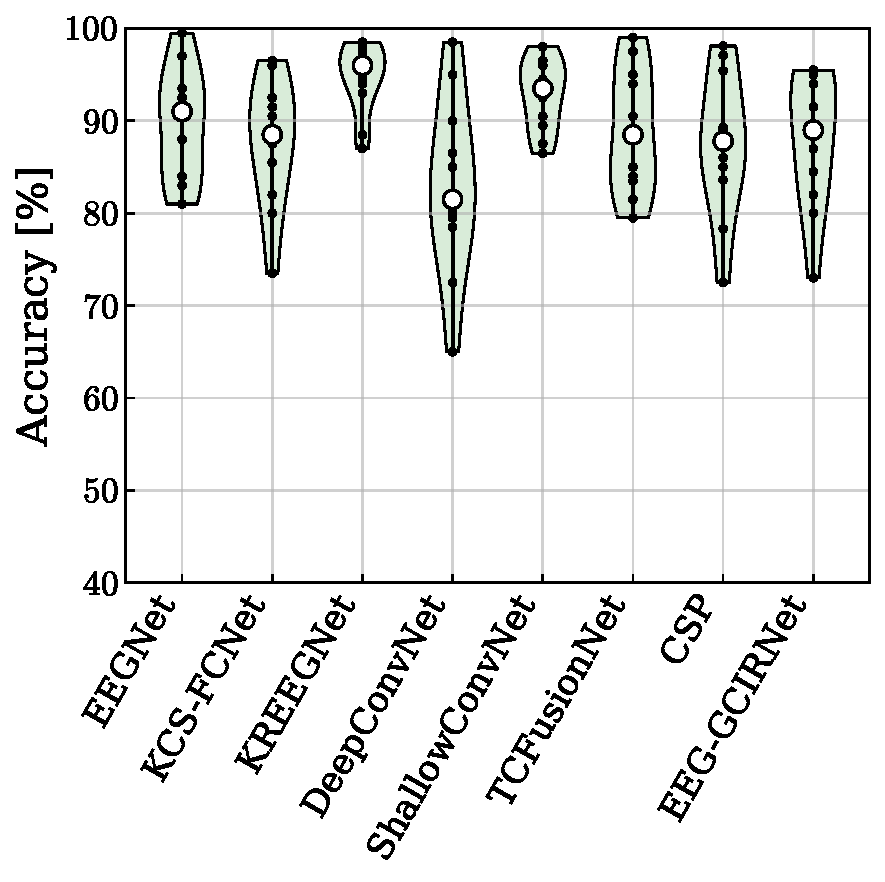
\includegraphics[height=4.5cm]{Figures/violin_good.pdf}}
%          \label{fig:violin_good}
%          \subfloat[]{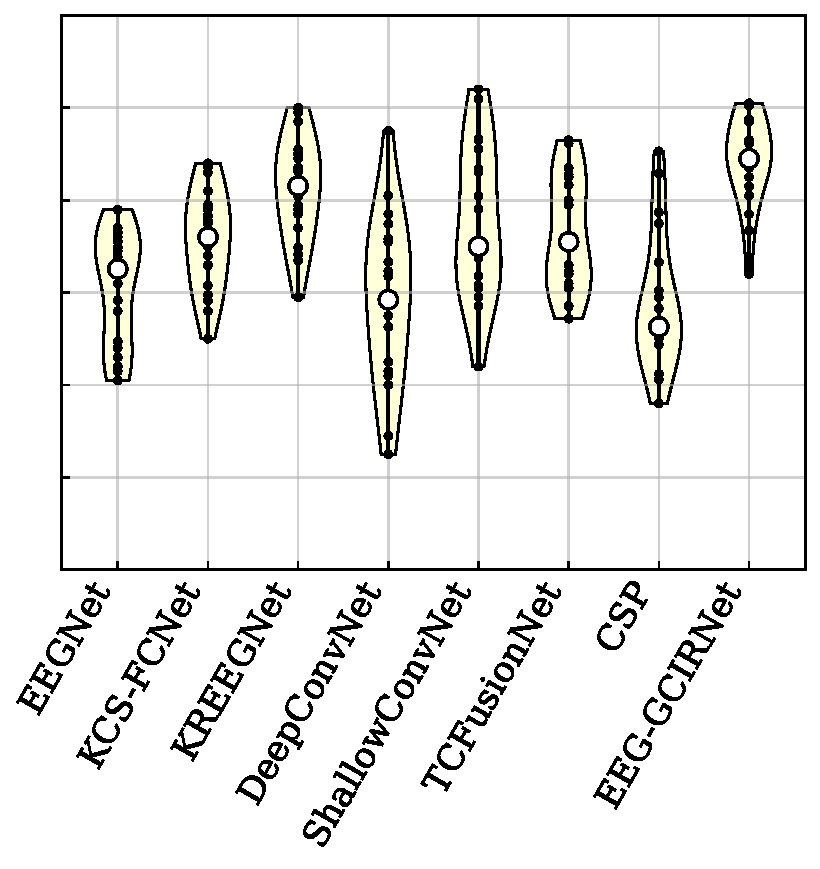
\includegraphics[height=4.5cm]{Figures/violin_mid.pdf}}
%          \label{fig:violin_mid}
%          \subfloat[]{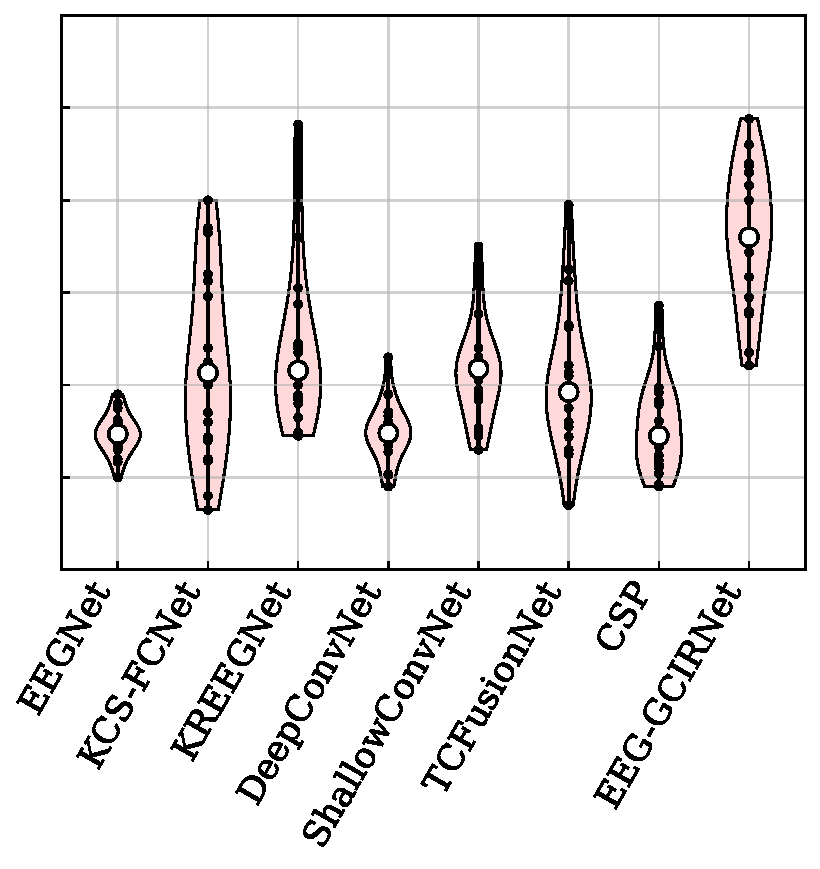
\includegraphics[height=4.5cm]{Figures/violin_bad.pdf}}
%          \label{fig:violin_bad}

%     \caption{Group performing MI-\gls{eeg}classification results. The white dot in each violin plot indicates the median accuracy, while the thick black bar represents the interquartile range. The corresponding average (mean) accuracies for EEGNet and EEG-GCIRNet are reported in Table~\ref{tab:accuracy_gain}.(\textbf{a})
%  Subjects with EEGNet accuracy above 80$\%$. (\textbf{b}) Subjects with EEGNet accuracy between 60$\%$ and 80$\%$. (\textbf{c}) Subjects with EEGNet accuracy below 60$\%$.}
%     \label{fig:Violins}
% \end{figure}
% %-----------------------------------------------
%-----------------------------------------------
\begin{figure}[htbp]
    \centering

    \subfloat[Subjects with EEGNet accuracy above 80\%.]{
        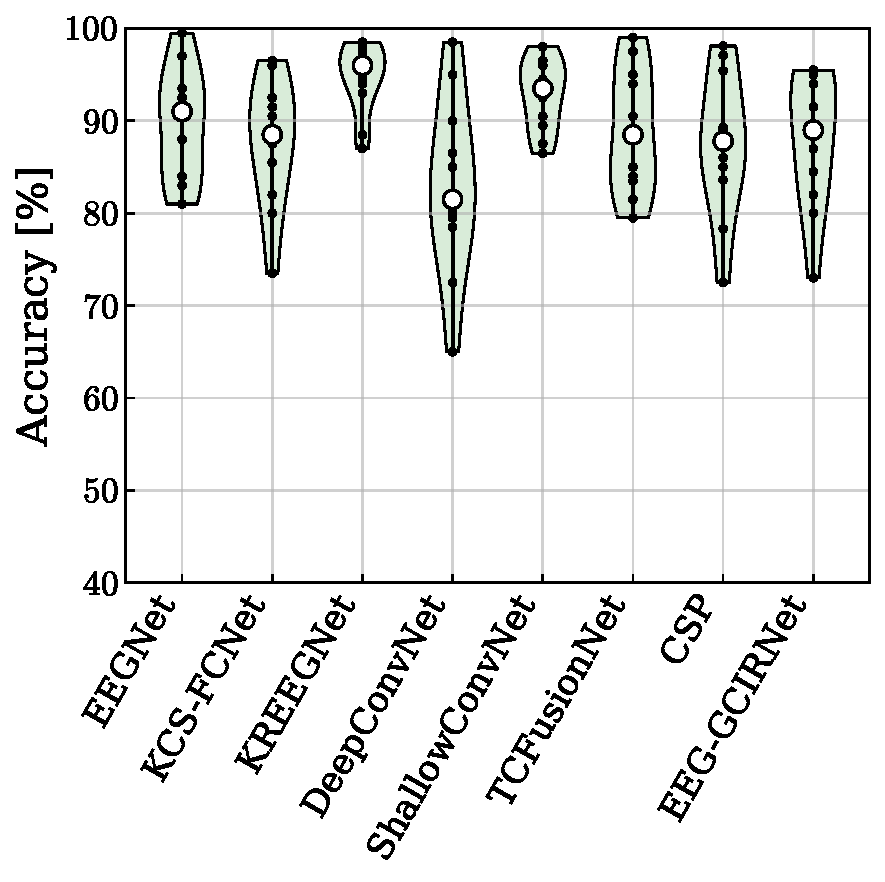
\includegraphics[height=4.8cm]{Figures/violin_good.pdf}
        \label{fig:violin_good}
    }
    \hfill
    \subfloat[Subjects with EEGNet accuracy between 60\% and 80\%.]{
        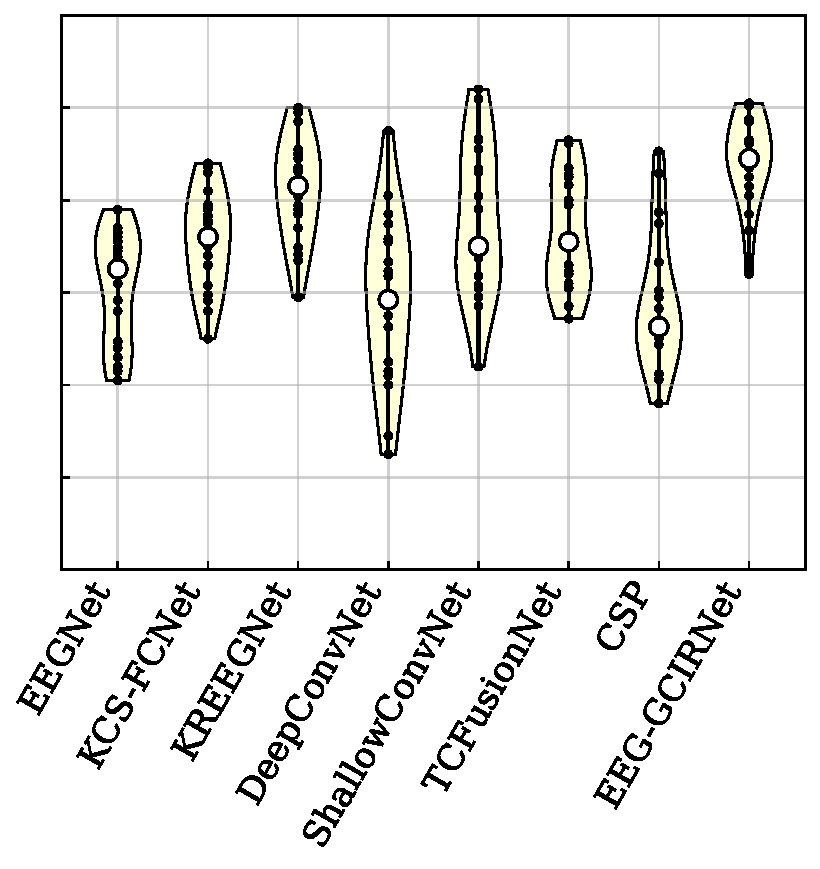
\includegraphics[height=4.8cm]{Figures/violin_mid.pdf}
        \label{fig:violin_mid}
    }
    \hfill
    \subfloat[Subjects with EEGNet accuracy below 60\%.]{
        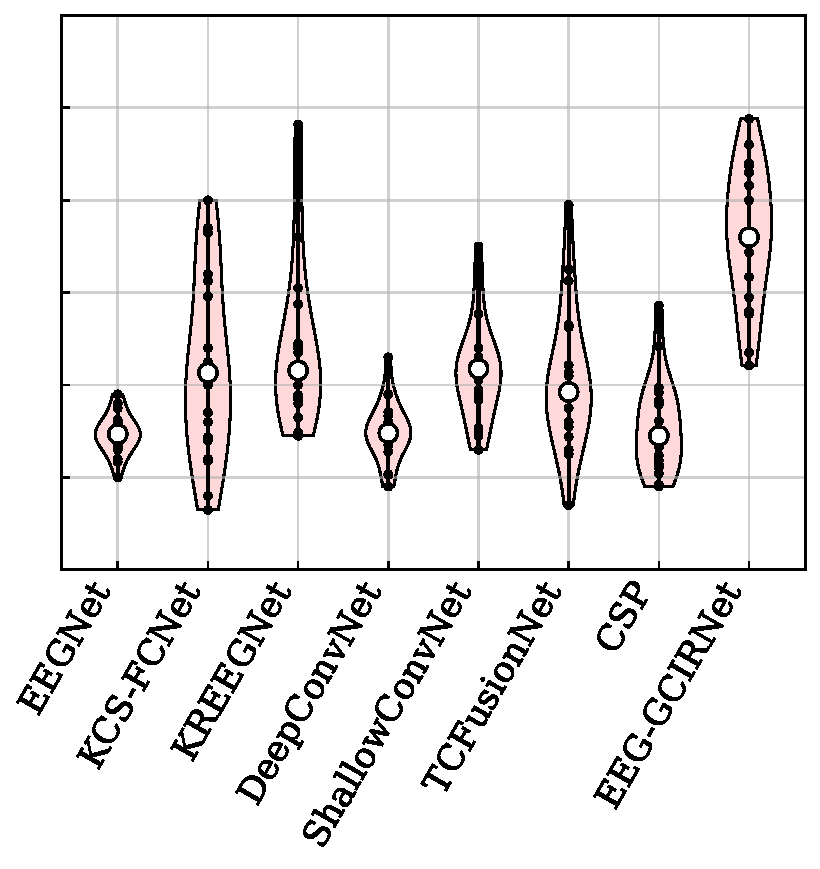
\includegraphics[height=4.8cm]{Figures/violin_bad.pdf}
        \label{fig:violin_bad}
    }

    \caption{Classification performance by subject group for the
    \gls{mi}-\gls{eeg} task. The white dot in each violin plot indicates
    the median accuracy, while the thick black bar represents the
    interquartile range. The corresponding mean accuracies for EEGNet
    and \gls{eeggcirnet} are reported in Table~\ref{tab:accuracy_gain}.}
    \label{fig:Violins}
\end{figure}
%-----------------------------------------------

The most compelling evidence of the model's robustness is found in the ``Bad'' group (Figure~\ref{fig:Violins}c), which reflects the most challenging \gls{eeg} conditions. Here, most models exhibit broad distributions shifted toward low accuracies (40--70\%). Crucially, \gls{eeggcirnet} is the only model for which this group is empty, reaffirming its resilience against signal degradation and its superior stability, as previously suggested by the global accuracy and ranking analyses.


These distributional advantages translate directly into substantial accuracy gains, as summarized in Table~\ref{tab:accuracy_gain}. The improvements are most pronounced for subjects who perform poorly with baseline models. In the ``Bad'' group, where EEGNet achieves an average accuracy of only 54.65\%, \gls{eeggcirnet} provides a remarkable $\sim$22\% increase, elevating the average performance to 76.20\%. A substantial gain of $\sim$14\% is also observed in the ``Mid'' group. Conversely, for the ``Good'' group, where the baseline performance is already high, \gls{eeggcirnet} maintains a comparable accuracy with only a slight decrease ($\sim$2\%). This confirms that the significant gains for challenging cases are not achieved at the expense of performance in high-quality signal conditions.

%------------------------------------------------
\begin{table}[H]%[htbp]
    \caption{Accuracy and gain by {subject performance group} and approach.}
   {
    \begin{tabularx}{\textwidth}{CCCC}
       \toprule
       \textbf{Approach} & \textbf{Group} & \textbf{Accuracy (\%)} & \textbf{Gain (\%)} \\
       \midrule
       \multirow{3}{*}{EEGNet}
         & Good    & 89.64 & --    \\
         & Mid     & 70.54 & --    \\
         & Bad     & 54.65 & --    \\
       \midrule
       \multirow{3}{*}{EEG-GCIRNet (Ours)}
         & Good    & 87.86 & $-1.78$     \\
         & Mid     & 84.24 & $13.70$    \\
         & Bad     & 76.20 & $21.55$    \\
       \bottomrule
    \end{tabularx}}
    \label{tab:accuracy_gain}
\end{table}
%------------------------------------------------
%------------------------------------------------
\begin{figure}[H]
  
\hspace{-12pt}  \resizebox{\linewidth}{!}{% --------- Dimensiones y colores ----------
\def\FigW{20cm}
\def\FigH{8.5cm}

\definecolor{EEGNetDark}{HTML}{7CD8E2}
\definecolor{EEGNetLight}{HTML}{CAEBF1}
\definecolor{CIRNetDark}{HTML}{98D891}
\definecolor{CIRNetLight}{HTML}{ABE3A1}

% --------- Estilos ----------
\pgfplotsset{
  myaxis/.style={
    width=\FigW, height=\FigH,
    ymin=40, ymax=100,
    ylabel={Accuracy [\%]},
    ylabel style={font=\small},
    ytick={40,60,...,100},
    xtick pos=bottom, ytick pos=left,
    tick align=inside,
    ticklabel style={font=\scriptsize},
    axis lines=box,
    tick style={black!60},
    xmajorgrids, ymajorgrids,
    grid style={black!15},
  },
  methodline/.style={
    line width=1.1pt,
    mark=*,
    mark size=1.6pt,
    mark options={solid, draw=#1, fill=#1},
    draw=#1
  },
  bandstyle/.style={draw=none, fill opacity=0.40},
}

% --------- Datos ---------
\pgfplotstableread[row sep=\\, col sep=space]{
subj  eegnet  nrvae  seeg  sgc \\
  43   99.50   94.00   4.64  4.64 \\
  14   97.00   95.50   1.87  1.87 \\
  3    93.50   93.00   4.06  6.00 \\
  50   92.50   84.50   4.58  4.58 \\
  48   92.50   95.00   2.24  2.24 \\
  4    91.00   92.00   6.12  4.80 \\
  35   88.00   82.00   6.96  6.96 \\
  23   84.00   89.00   3.39  3.39 \\
  13   84.00   87.00   2.45  2.45 \\
  41   83.00   80.00   7.75  7.75 \\
  1    81.00   75.00   5.10  5.70 \\
  49   78.97   90.26   2.99  2.99 \\
  37   77.00   85.00   7.31  6.52 \\
  26   76.50   88.50   5.15  3.00 \\
  5    76.50   84.50   7.35  6.20 \\
  44   76.00   90.50   5.61  5.34 \\
  6    75.56   76.67   4.51  4.51 \\
  47   74.87   90.26   5.23  2.51 \\
  28   74.50   86.50   6.96  5.39 \\
  36   73.85   86.15   2.99  4.76 \\
  12   72.57   72.00   7.54  7.54 \\
  39   71.00   78.50   6.04  6.04 \\
  46   69.17   88.75   4.64  1.67 \\
  10   68.00   86.50   9.41  8.15 \\
  20   64.71   83.53   3.72  6.86 \\
  22   64.00   82.50   6.44  6.12 \\
  31   63.00   84.00   9.92  6.44 \\
  18   62.00   84.50   5.34  4.85 \\
  52   61.50   80.50   6.63  8.86 \\
  25   60.50   81.50   11.11 6.25 \\
  21   59.00   84.00   4.64  4.64 \\
  40   58.00   80.00   9.62  9.62 \\
  24   57.50   83.00   4.85  4.85 \\
  27   56.22   62.16   6.71  6.40 \\
  30   56.00   81.60   8.24  8.24 \\
  51   55.90   74.36   3.40  7.78 \\
  42   55.50   86.00   5.83  5.83 \\
  16   55.00   76.00   10.56 10.56 \\
  9    55.00   83.75   3.33  3.33 \\
  38   54.87   67.69   7.71  7.71 \\
  11   54.50   75.50   8.28  8.28 \\
  19   54.48   71.72   9.61  9.61 \\
  33   54.00   76.00   4.64  3.00 \\
  2    54.00   76.00   9.95  10.68 \\
  17   53.50   69.50   3.74  9.41 \\
  15   53.33   80.00   4.10  2.51 \\
  45   53.00   68.00   6.60  5.34 \\
  32   52.00   63.50   8.57  4.64 \\
  7    51.67   88.75   10.32 10.83 \\
  8    50.00   76.50   8.22  5.15 \\
}\datatable

\begin{tikzpicture}
\begin{axis}[
  myaxis,
  enlarge x limits=0,
  enlarge y limits=false,
  trim axis left, trim axis right,
  xlabel={Subjects},
  symbolic x coords={
    43,14,3,50,48,4,35,23,13,41,1,49,37,26,5,44,6,47,28,36,12,39,46,10,
    20,22,31,18,52,25,21,40,24,27,30,51,42,16,9,38,11,19,33,2,17,15,45,32,7,8
  },
  xtick=data,
  x tick label style={rotate=90, anchor=east},
  legend style={
    at={(rel axis cs:0.001,0.001)}, anchor=south west,
    draw=black!40, fill=white, fill opacity=0.9, font=\small,
    rounded corners=2pt
  },
  legend cell align=left,
]

% ===== EEGNet (banda + línea) =====
\addplot[name path=EEGNetUpper, draw=none, forget plot]
  table [x=subj, y expr=\thisrow{eegnet}+\thisrow{seeg}] {\datatable};
\addplot[name path=EEGNetLower, draw=none, forget plot]
  table [x=subj, y expr=\thisrow{eegnet}-\thisrow{seeg}] {\datatable};
\addplot[bandstyle, fill=EEGNetLight, forget plot]
  fill between[of=EEGNetUpper and EEGNetLower];
\addplot[methodline={EEGNetDark}]
  table [x=subj, y=eegnet] {\datatable};

% ===== EEG-CIRNet (banda + línea) =====
\addplot[name path=CIRNetUpper, draw=none, forget plot]
  table [x=subj, y expr=\thisrow{nrvae}+\thisrow{sgc}] {\datatable};
\addplot[name path=CIRNetLower, draw=none, forget plot]
  table [x=subj, y expr=\thisrow{nrvae}-\thisrow{sgc}] {\datatable};
\addplot[bandstyle, fill=CIRNetLight, forget plot]
  fill between[of=CIRNetUpper and CIRNetLower];
\addplot[methodline={CIRNetDark}]
  table [x=subj, y=nrvae] {\datatable};

% ===== Leyenda con el MISMO color de las líneas =====
\addlegendimage{line legend, draw=EEGNetDark, mark=*}
\addlegendentry{EEGNet}
\addlegendimage{line legend, draw=CIRNetDark, mark=*}
\addlegendentry{EEG-GCIRNet}

\end{axis}
\end{tikzpicture}}
  \caption{Inter-subject classification accuracies of EEGNet and \gls{eeggcirnet}. Each point represents the average performance per subject, with subjects ordered according to EEGNet accuracy to highlight the comparative improvements achieved by \gls{eeggcirnet}. Shaded regions indicate \mbox{performance variability}.}
  \label{fig:gains}
\end{figure}
Figure~\ref{fig:gains} illustrates the subject-specific improvements of \gls{eeggcirnet} over the EEGNet baseline, providing direct visual evidence of our framework's corrective capability. Since the performance groups were stratified based on EEGNet's accuracy, the figure demonstrates our model's ability to significantly elevate the performance of users who struggle with conventional BCI systems, thereby directly addressing the challenge of BCI illiteracy. While most participants benefit from moderate accuracy gains, a notable subset—including subjects $21$, $40$, $24$, $30$, $42$, $9$, $15$, and $7$ exhibit a pronounced transition from ``Bad'' to ``Good'' performance levels. For several of these individuals (e.g., subjects $24$, $9$, and $7$), accuracy exceeds the $80\%$ threshold. This performance leap reinforces the hypothesis that latent space modeling in \gls{eeggcirnet} not only mitigates the limitations of signal noise but also provides an effective mechanism for uncovering discriminative structure in signals previously deemed uninformative.

These findings are highly relevant for developing inclusive BCI systems. The fact that several initially low-performing individuals achieve high accuracy suggests that \gls{eeggcirnet} can serve a corrective function within BCI pipelines, enhancing usability and consistency. This benefit extends to ``Mid-performing'' users as well, many of whom are elevated to the high-performing category. This corrective and enhancing capability supports the use of latent generative models in real-world BCI contexts, where adaptability and generalization are critical~\cite{nagarajan2024deeptransfer, gomez2021kernelcca, demir2021autobayes}.

%------------------------------------------------
\subsubsection{Validation on Canonical Scenarios: Binary \gls{mi} Decoding on BCI Competition IV-2a}

The BCI Competition IV-2a dataset constitutes a canonical benchmark for binary \gls{mi} decoding, where the task is restricted to discriminating between left-hand and right-hand \gls{mi} under controlled experimental conditions. In contrast to the multi-class and subject-group validation scenarios analyzed on \gls{eegmmidb} and \gls{adhd}, this dataset enables a direct assessment of the proposed framework’s ability to capture discriminative neural patterns within a highly standardized and widely adopted reference setting in the literature.

The comparative results reported in Table~\ref{tab:acc_comparison} demonstrate that \gls{eeggcirnet} achieves an average accuracy of 88.56\%, placing it among the top-performing methods reported for this binary decoding scenario. This performance clearly surpasses that of widely used convolutional architectures such as EEGNet, DeepConvNet, and ShallowConvNet, which typically achieve accuracies in the 65–68\% range, as well as approaches based on statistical features and classical ensemble strategies, whose performance remains below 65\%.

When compared with more recent methods that incorporate connectivity information or attention-based mechanisms, such as GAT+PLV, \gls{eeggcirnet} exhibits a substantial improvement, with an approximate gain of 16.7 percentage points. This increase suggests that integrating functional connectivity representations structured as topographic maps provides a significant advantage even in binary classification scenarios, where decision boundaries are relatively simpler than those encountered in multi-class \gls{mi} tasks.

%---------------------------------------------------------------------------------
\begin{figure}[htbp]
 \hspace{-12pt}\resizebox{\linewidth}{!}{%

% --------- Dimensiones y colores ----------
\def\FigW{20cm}
\def\FigH{8.5cm}

\definecolor{EEGNetDark}{HTML}{7CD8E2}
\definecolor{EEGNetLight}{HTML}{CAEBF1}
\definecolor{CIRNetDark}{HTML}{98D891}
\definecolor{CIRNetLight}{HTML}{ABE3A1}

% --------- Estilos ----------
\pgfplotsset{
  myaxis/.style={
    width=\FigW, height=\FigH,
    ymin=45, ymax=101,
    ylabel={Accuracy [\%]},
    ylabel style={font=\small},
    ytick={45,50,60,70,80,90,100},
    xtick pos=bottom, ytick pos=left,
    tick align=inside,
    ticklabel style={font=\scriptsize},
    axis lines=box,
    tick style={black!60},
    xmajorgrids, ymajorgrids,
    grid style={black!15},
  },
  methodline/.style={
    line width=1.1pt,
    mark=*,
    mark size=1.6pt,
    mark options={solid, draw=#1, fill=#1},
    draw=#1
  },
  bandstyle/.style={draw=none, fill opacity=0.40},
}

% --------- Datos (ordenados por ACC EEGNet de MAYOR a MENOR) ---------
\pgfplotstableread[row sep=\\, col sep=space]{
subj  eegnet  eegnet_std   cir   cir_std \\
9     74.14   0.00         100.00 0.00 \\
8     70.69   0.00         100.00 0.00 \\
7     70.69   0.00         83.33  0.00 \\
6     65.52   0.00         89.13  0.00 \\
5     63.79   0.00         80.77  0.00 \\
3     63.79   0.00         91.07  0.00 \\
1     63.79   0.00         92.86  0.00 \\
4     55.17   0.00         82.69  0.00 \\
2     46.55   0.00         73.21  0.00 \\
}\datatable

\begin{tikzpicture}
\begin{axis}[
  myaxis,
  enlarge x limits=0,
  xlabel={Subjects},
  symbolic x coords={9,8,7,6,5,3,1,4,2},
  xtick=data,
  x tick label style={rotate=90, anchor=east},
  legend style={
    at={(rel axis cs:0.001,0.001)}, anchor=south west,
    draw=black!40, fill=white, fill opacity=0.9, font=\small,
    rounded corners=2pt
  },
  legend cell align=left,
]

% ===== EEGNet =====
\addplot[name path=EEGNetUpper, draw=none, forget plot]
  table [x=subj, y expr=\thisrow{eegnet}+\thisrow{eegnet_std}] {\datatable};

\addplot[name path=EEGNetLower, draw=none, forget plot]
  table [x=subj, y expr=\thisrow{eegnet}-\thisrow{eegnet_std}] {\datatable};

\addplot[bandstyle, fill=EEGNetLight, forget plot]
  fill between[of=EEGNetUpper and EEGNetLower];

\addplot[methodline={EEGNetDark}]
  table [x=subj, y=eegnet] {\datatable};

% ===== EEG-GCIRNet =====
\addplot[name path=CIRNetUpper, draw=none, forget plot]
  table [x=subj, y expr=\thisrow{cir}+\thisrow{cir_std}] {\datatable};

\addplot[name path=CIRNetLower, draw=none, forget plot]
  table [x=subj, y expr=\thisrow{cir}-\thisrow{cir_std}] {\datatable};

\addplot[bandstyle, fill=CIRNetLight, forget plot]
  fill between[of=CIRNetUpper and CIRNetLower];

\addplot[methodline={CIRNetDark}]
  table [x=subj, y=cir] {\datatable};

% ===== Leyenda =====
\addlegendimage{line legend, draw=EEGNetDark, mark=*}
\addlegendentry{EEGNet}

\addlegendimage{line legend, draw=CIRNetDark, mark=*}
\addlegendentry{EEG-GCIRNet}

\end{axis}
\end{tikzpicture}
}
\caption{{Inter-subject classification accuracies for EEGNet and EEG-GCIRNet on BCI Competition IV-2a. Subjects are ordered according to their EEGNet accuracy.}}
\label{fig:acc_eegnet_vs_eegcirnet_bcic2a}
\end{figure}
%---------------------------------------------------------------------------------

Beyond the aggregate performance comparison summarized in Table~\ref{tab:acc_comparison}, a more fine-grained subject-wise analysis is provided in Fig.~\ref{fig:acc_eegnet_vs_eegcirnet_bcic2a}. This figure contrasts the inter-subject accuracies obtained by EEGNet and the proposed \gls{eeggcirnet} on the BCI Competition IV-2a dataset, with subjects ordered according to EEGNet performance. The visualization reveals that \gls{eeggcirnet} consistently outperforms EEGNet across all subjects, including those exhibiting lower baseline accuracies under the conventional convolutional architecture. Notably, the largest performance gains are observed for subjects with poorer EEGNet performance, indicating an enhanced robustness of the proposed connectivity-driven representation to inter-subject variability. These results suggest that modeling functional connectivity through structured topographic maps allows \gls{eeggcirnet} to capture subject-specific discriminative patterns that are insufficiently exploited by purely channel-wise convolutional approaches, even in canonical binary \gls{mi} decoding scenarios.

It is also noteworthy that the performance of \gls{eeggcirnet} is comparable to that of high-complexity models such as CTNet and CNNViT-MILF-a, which report similarly high accuracies but, in some cases, on different datasets (BCI Competition IV-2b) or using considerably heavier architectures. In this context, the results obtained by \gls{eeggcirnet} reinforce the notion that an informative and physiologically consistent representation can be as decisive as increasing architectural complexity in achieving high performance for \gls{mi} decoding.

%-------------------------------------------------------------------------
\begin{table}[H]
    \centering
    \caption{Average classification accuracy of state-of-the-art methods for binary MI-\gls{eeg} decoding (Left vs. Right) on BCI Competition IV Dataset IIa.}
    \label{tab:acc_comparison}
    \begin{tabularx}{\textwidth}{CC}
        \toprule
        \textbf{Model} & \textbf{ACC [\%]} \\
        \midrule
        DeepConvNet~\cite{schirrmeister2017deep} 
        & $67.62$ \\
        
        ShallowConvNet~\cite{schirrmeister2017deep} 
        & $66.41$ \\
        
        EEGNet~\cite{lawhern2018eegnet} 
        & $65.49$ \\
        
        TE$\kappa_\alpha$~\cite{de2019data} 
        & $68.80$ \\
        
        StatFeat-Ensemble v1~\cite{Degirmenci2023} 
        & $61.86$ \\
        
        StatFeat-Ensemble v2~\cite{Degirmenci2024} 
        & $63.04$ \\
        
        GAT+PLV~\cite{patel2025advancing} 
        & $71.89$ \\
        
        CTNet$^{\dagger}$~\cite{CTNet} 
        & $88.49$ \\
        
        CNNViT\text{-}MILF\text{-}a$^{\dagger}$~\cite{CNNViT} 
        & $81.11$ \\
        
        \textbf{EEG-GCIRNet (Ours)} 
        & $\mathbf{88.56}$ \\
        \bottomrule
    \end{tabularx}

    \vspace{4pt}
    \footnotesize{\textbf{Note.} $^{\dagger}$ Accuracy reported on BCI Competition IV-2b for two-class left/right motor imagery classification.}
\end{table}
%-------------------------------------------------------------------------

\subsubsection{Validation on Complex Scenarios: Multi-Class Decoding on \gls{eegmmidb} Collection}

{To assess the scalability of the proposed framework beyond binary classification, we evaluated its performance on the \gls{eegmmidb} dataset, which involves a challenging $5$-class \gls{mi} task. This scenario requires the model to disentangle multiple distinct neural patterns (Left Hand, Right Hand, Both Hands, Both Feet, and Rest), significantly increasing the complexity of the decision boundaries compared to the GigaScience benchmark.}

{Table~\ref{tab:acc_5class_results} presents the comparative results against a curated set of state-of-the-art architectures. These baselines were selected to represent the broad spectrum of current deep learning strategies for \gls{eeg}decoding: {EEGNet} serves as the compact, general-purpose benchmark; {DeepConvNet} and {ShallowConvNet} represent established end-to-end architectures that optimize temporal and spatial filters directly from raw data; and {TCFusionNet} is included to represent recent advancements in complex temporal-channel fusion mechanisms. Against this diverse backdrop of raw signal decoders, \gls{eeggcirnet} achieves the highest average accuracy of $75.20 \pm 4.63\%$, surpassing all baseline models by a considerable margin. While reference architectures such as TCFusionNet and DeepConvNet plateau around $\sim 68\%$ (with $68.89\%$ and $68.35\%$ respectively), our approach yields a net performance gain of approximately $6.3\%$. This superiority is particularly notable given the difficulty of the task, suggesting that the connectivity-driven topographic maps provide a richer feature space than raw temporal signals for distinguishing between spatially overlapping classes, such as ``Both Hands'' versus single-hand imagery.}

\begin{table}[H]%[ht!]
    
    \caption{{MI-\gls{eeg}5-class classification performance comparison: 
    Average ACC $\pm$ standard deviation across the $10$ considered subjects.}}
    {
    \begin{tabularx}{\textwidth}{CC}
        \toprule
        \textbf{Model} & \textbf{ACC [\%]} \\
        \midrule
        % CSP~\cite{ang2008filter} &  \\
        EEGNet~\cite{lawhern2018eegnet} & $67.94 \pm 3.98$ \\
        % KREEGNet~\cite{computers12070145} &  \\
        % KCS-FCNet~\cite{diagnostics13061122} &  \\
        DeepConvNet~\cite{schirrmeister2017deep} & $68.35 \pm 4.11$ \\
        ShallowConvNet~\cite{Kim2022} & $67.90 \pm 4.06$ \\
        TCFusionNet~\cite{Musallam2021} & $68.89 \pm 3.90$ \\
        \textbf{EEG-GCIRNet (Ours)} & $\mathbf{75.20 \pm 4.63}$ \\
        \bottomrule
    \end{tabularx}}
    \label{tab:acc_5class_results}
\end{table}

The robustness of these findings is visually confirmed in Figure~\ref{fig:acc_5}, which details subject-wise accuracy sorted by baseline performance. \gls{eeggcirnet} maintains a strict performance advantage across the entire cohort, with the green curve remaining consistently above the baseline. This superiority is particularly pronounced for the most challenging subjects (e.g., Subjects 8, 49, and 7); while the baseline model's performance degrades towards $65\%$, the proposed framework exhibits a corrective behavior, stabilizing accuracies above $71\%$ achieving the highest accuracy with $\sim$78\% for subject 7. Furthermore, the narrower confidence intervals (shaded regions) observed for \gls{eeggcirnet} indicate that the variational regularization effectively mitigates the variability inherent in complex 5-class decision boundaries, yielding not only higher accuracy but greater predictive stability than standard temporal decoding.

Overall, these results confirm that the proposed unimodal VAE framework is not limited to simple binary discrimination but effectively scales to multi-class scenarios, leveraging the latent disentanglement of connectivity patterns to resolve complex \gls{mi} tasks.

\begin{figure}[H]
  
 \hspace{-12pt} \resizebox{\linewidth}{!}{% --------- Dimensiones y colores ----------
\def\FigW{20cm}
\def\FigH{8.5cm}

\definecolor{EEGNetDark}{HTML}{7CD8E2}
\definecolor{EEGNetLight}{HTML}{CAEBF1}
\definecolor{CIRNetDark}{HTML}{98D891}
\definecolor{CIRNetLight}{HTML}{ABE3A1}

% --------- Estilos (MISMO DEL ORIGINAL) ----------
\pgfplotsset{
  myaxis/.style={
    width=\FigW, height=\FigH,
    ymin=60, ymax=80,
    ylabel={Accuracy [\%]},
    ylabel style={font=\small},
    ytick={60,65,70,75,80, 85},
    xtick pos=bottom, ytick pos=left,
    tick align=inside,
    ticklabel style={font=\scriptsize},
    axis lines=box,
    tick style={black!60},
    xmajorgrids, ymajorgrids,
    grid style={black!15},
  },
  methodline/.style={
    line width=1.1pt,
    mark=*,
    mark size=1.6pt,
    mark options={solid, draw=#1, fill=#1},
    draw=#1
  },
  bandstyle/.style={draw=none, fill opacity=0.40},
}

% --------- Datos ordenados por ACC EEGNet ---------
\pgfplotstableread[row sep=\\, col sep=space]{
subj  eegnet  eegnet_std   cir   cir_std \\
13  70.1587  3.0778   77.79  3.7022 \\
50  70.1587  2.7309   77.80  4.0902 \\
12  69.5238  3.9396   77.77  6.8824 \\
9   69.2063  3.8359   76.19  5.0195 \\
40  68.2539  3.3295   76.18  7.0702 \\
7   67.3016  3.8359   77.78  5.4618 \\
41  66.3492  5.2549   71.44  3.5634 \\
49  66.3492  5.2549   73.01 3.4191 \\
3   66.0317  5.0793   71.43  2.5790 \\
8   66.0317  4.7724   73.02  4.4895 \\
}\datatable


\begin{tikzpicture}
\begin{axis}[
  myaxis,
  enlarge x limits=0,
  xlabel={Subjects},
  symbolic x coords={13,50,12,9,40,7,41,49,3,8},
  xtick=data,
  x tick label style={rotate=90, anchor=east},
  legend style={
    at={(rel axis cs:0.001,0.001)}, anchor=south west,
    draw=black!40, fill=white, fill opacity=0.9, font=\small,
    rounded corners=2pt
  },
  legend cell align=left,
]

% ===== EEGNet =====
\addplot[name path=EEGNetUpper, draw=none, forget plot]
  table [x=subj, y expr=\thisrow{eegnet}+\thisrow{eegnet_std}] {\datatable};

\addplot[name path=EEGNetLower, draw=none, forget plot]
  table [x=subj, y expr=\thisrow{eegnet}-\thisrow{eegnet_std}] {\datatable};

\addplot[bandstyle, fill=EEGNetLight, forget plot]
  fill between[of=EEGNetUpper and EEGNetLower];

\addplot[methodline={EEGNetDark}]
  table [x=subj, y=eegnet] {\datatable};

% ===== EEG-GCIRNet =====
\addplot[name path=CIRNetUpper, draw=none, forget plot]
  table [x=subj, y expr=\thisrow{cir}+\thisrow{cir_std}] {\datatable};

\addplot[name path=CIRNetLower, draw=none, forget plot]
  table [x=subj, y expr=\thisrow{cir}-\thisrow{cir_std}] {\datatable};

\addplot[bandstyle, fill=CIRNetLight, forget plot]
  fill between[of=CIRNetUpper and CIRNetLower];

\addplot[methodline={CIRNetDark}]
  table [x=subj, y=cir] {\datatable};

% ===== Leyenda EXACTAMENTE como el código original =====
\addlegendimage{line legend, draw=EEGNetDark, mark=*}
\addlegendentry{EEGNet}

\addlegendimage{line legend, draw=CIRNetDark, mark=*}
\addlegendentry{EEG-GCIRNet}

\end{axis}
\end{tikzpicture}
}
  \caption{{Inter-subject classification accuracies for EEGNet and \gls{eeggcirnet} in the 5-class MI-\gls{eeg}setting. Subjects are ordered according to their EEGNet accuracy to emphasize the consistent performance gains achieved by \gls{eeggcirnet}. Shaded regions denote the accuracy variability \mbox{across trials.}}}
  \label{fig:acc_5}
\end{figure}

{For the multi-class setting, we analyzed the stability of the models through average rankings and assessed the significance of the performance differences using pairwise Wilcoxon signed-rank tests. The summary of these statistical metrics is presented in Table~\ref{tab:p-values_updated1}. \gls{eeggcirnet} achieves a perfect average ranking of ${1.00}$, indicating that it consistently outperformed all reference architectures across the considered subjects. This places it significantly ahead of the nearest competitor, TCFusionNet, which obtained an average ranking of $2.15$, and well beyond the standard end-to-end baselines like DeepConvNet ($3.10$) and EEGNet ($4.30$). The statistical reliability of these gains is confirmed by the hypothesis testing analysis. The proposed model yields the lowest average $p$-value (${0.002}$), which is markedly below the standard significance threshold ($\alpha = 0.05$). While TCFusionNet and DeepConvNet also exhibit statistical significance ($p=0.021$ and $p=0.026$, respectively), the order-of-magnitude difference in favor of \gls{eeggcirnet} underscores its robustness. Conversely, shallow and compact architectures such as ShallowConvNet and EEGNet show high $p$-values ($0.25$), suggesting that their performance fluctuations in this complex 5-class scenario lack statistical consistency compared to the proposed approach.}
%-----------------------------------------------
\begin{table}[H]%[ht!]
    \centering
    \caption{Average rankings and average pairwise Wilcoxon $p$-values.}
    \begin{tabularx}{\textwidth}{CCC}
       \toprule
        \textbf{Model} & \textbf{Avg. Ranking} & \textbf{Avg. Wilcoxon \emph{p}-Value} \\
        \midrule
        EEGNet        & $4.30$ & $0.25$ \\
        DeepConvNet   & $3.10$ & $0.026$ \\
        ShallowConvNet& $4.45$ & $0.25$ \\
        TCFusion      & $2.15$ & $0.021$ \\
        \textbf{EEG-GCIRNet (Ours)} & $\mathbf{1.00}$ & $\mathbf{0.002}$ \\
        \bottomrule
    \end{tabularx}
    \label{tab:p-values_updated1}
\end{table}
%-----------------------------------------------

\subsubsection{Subject-Group Validation on the \gls{adhd}/Control Children Dataset Following the SGKF-CV Protocol}

To further assess the generalization capability of the proposed framework under clinically realistic conditions, its performance was evaluated on the \gls{adhd}/control children dataset using a Subject-Group K-Fold Cross-Validation (SGKF-CV) protocol. Unlike conventional random or subject-dependent splits, the SGKF scheme enforces a strict separation of subjects between training and testing folds, thereby preventing any subject overlap. This validation setting poses a substantially more challenging scenario, as it explicitly evaluates the ability of the model to generalize across heterogeneous individuals rather than exploiting subject-specific \gls{eeg}patterns.

Table~\ref{tab:sgkf_accuracy_comparison} reports the accuracy-based performance comparison against a representative set of baseline models spanning classical machine learning methods and modern deep learning architectures for \gls{eeg}decoding. Under this stringent subject-independent evaluation, \gls{eeggcirnet} achieves an average accuracy of $63.50 \pm 3.44\%$. While this result is lower than those obtained by architectures such as T-GARNet, ShallowConvNet, and CNN-LSTM, it provides important insight into the behavior of connectivity-driven representations when confronted with pronounced inter-subject variability, which is characteristic of pediatric \gls{adhd} cohorts.

It is important to note that, in the \gls{adhd}/control children dataset, the dominant source of difficulty shifts from class separability—as observed in the multi-class \gls{eegmmidb} experiments—toward robust subject-to-subject transfer. In this context, performance improvements depend not only on the expressive power of the learned features but also on their invariance across subjects, recording sessions, and neurophysiological profiles. The observed performance gap relative to top-performing baselines suggests that additional mechanisms aimed at reducing domain shift, such as explicit domain alignment or adaptive normalization strategies, may be required to fully exploit connectivity-based representations in this setting. Nevertheless, the relatively moderate standard deviation across folds indicates that \gls{eeggcirnet} maintains stable behavior under SGKF-CV, highlighting its training robustness despite the challenging validation protocol.

Overall, these results confirm that the \gls{adhd}/control children dataset constitutes a substantially more demanding generalization scenario compared to subject-dependent or multi-class decoding tasks. While the proposed connectivity-driven framework demonstrates consistent and stable performance under strict subject-group validation, the comparison in Table~\ref{tab:sgkf_accuracy_comparison} also delineates clear opportunities for enhancing inter-subject robustness in clinical \gls{eeg}decoding applications, which remains a central challenge for practical BCI deployment.

%-------------------------------------------------------------------------
\begin{table}[H]
    \centering
    \caption{Performance comparison under the SGKF-CV protocol using accuracy as the evaluation metric. Accuracy is reported as mean $\pm$ standard deviation.}
    \label{tab:sgkf_accuracy_comparison}
    \begin{tabularx}{\textwidth}{CC}
        \toprule
        \textbf{Model} & \textbf{ACC [\%]} \\
        \midrule
        T-GARNet~\cite{salazar2025tgarnet} 
        & $\mathbf{82.07 \pm 3.07}$ \\
        
        ShallowConvNet~\cite{schirrmeister2017deep} 
        & $81.91 \pm 1.36$ \\
        
        CNN-LSTM~\cite{wang2022cnnlstm_adhd} 
        & $80.21 \pm 3.96$ \\
        
        EEGNet~\cite{lawhern2018eegnet} 
        & $75.61 \pm 4.60$ \\
        
        Multi-Stream Transformer~\cite{delvigne2022icpr_transformer_attention} 
        & $73.39 \pm 5.94$ \\
        
        ANOVA-PCA SVM~\cite{alim2023signals_anovapca_svm} 
        & $66.47 \pm 0.00$ \\
        
        IM-CBGT~\cite{alsharif2024aims_imcbgt} 
        & $64.98 \pm 0.78$ \\
        
        \textbf{EEG-GCIRNet ({Ours})} 
        & $63.50 \pm 3.44$ \\
        \bottomrule
    \end{tabularx}
\end{table}
%-------------------------------------------------------------------------

% \subsubsection{Interpretability and Internal Model Dynamics}

% To understand the mechanisms behind EEG-GCIRNet's robust performance, we analyzed its internal dynamics and learned representations. The results reveal that the model is not a ``black box'' but a structured framework that adapts its learning strategy, captures physiologically meaningful patterns, and creates an effective feature space.

To understand the mechanisms behind \gls{eeggcirnet}'s robust performance, we analyzed its internal dynamics and learned representations. The results reveal that the model is not a ``black box'', but rather a structured framework that adapts its learning strategy, captures physiologically meaningful patterns, and creates an effective feature space. {This interpretability analysis is organized around three complementary perspectives: the reorganization of the loss-function weights, the behavior of the latent space, and the temporal, spatial, and spectral patterns learned by the model. Together, these analyses provide insight into how \gls{eeggcirnet} balances reconstruction, classification, and regularization while preserving discriminative EEG information across different subject-performance groups.}

{This subsection provides an integrated analysis of how \gls{eeggcirnet} organizes its internal representations during training and how these representations support robust MI decoding. Rather than evaluating interpretability only through post-hoc visual explanations, the analysis considers complementary aspects of the model behavior, including the reorganization of loss-function weights, the balance between reconstruction and classification objectives, the structure of the latent space, and the temporal, spatial, and spectral patterns learned by the network. Together, these elements allow the model dynamics to be interpreted not only in terms of predictive performance, but also in terms of how discriminative and physiologically meaningful EEG information is preserved across different subject-performance groups.}

{In this sense, the interpretability analysis aims to show whether the proposed framework learns stable connectivity-driven representations, whether these representations remain consistent under different levels of subject variability, and whether the model relies on EEG patterns that are compatible with known MI-related neurophysiological mechanisms. The following subsections therefore examine the internal behavior of \gls{eeggcirnet} from multiple complementary perspectives.}

\subsubsection{Adaptive Learning Through Loss Weight Reorganization}
%------------------------------------------------
\begin{figure}[H]
    
    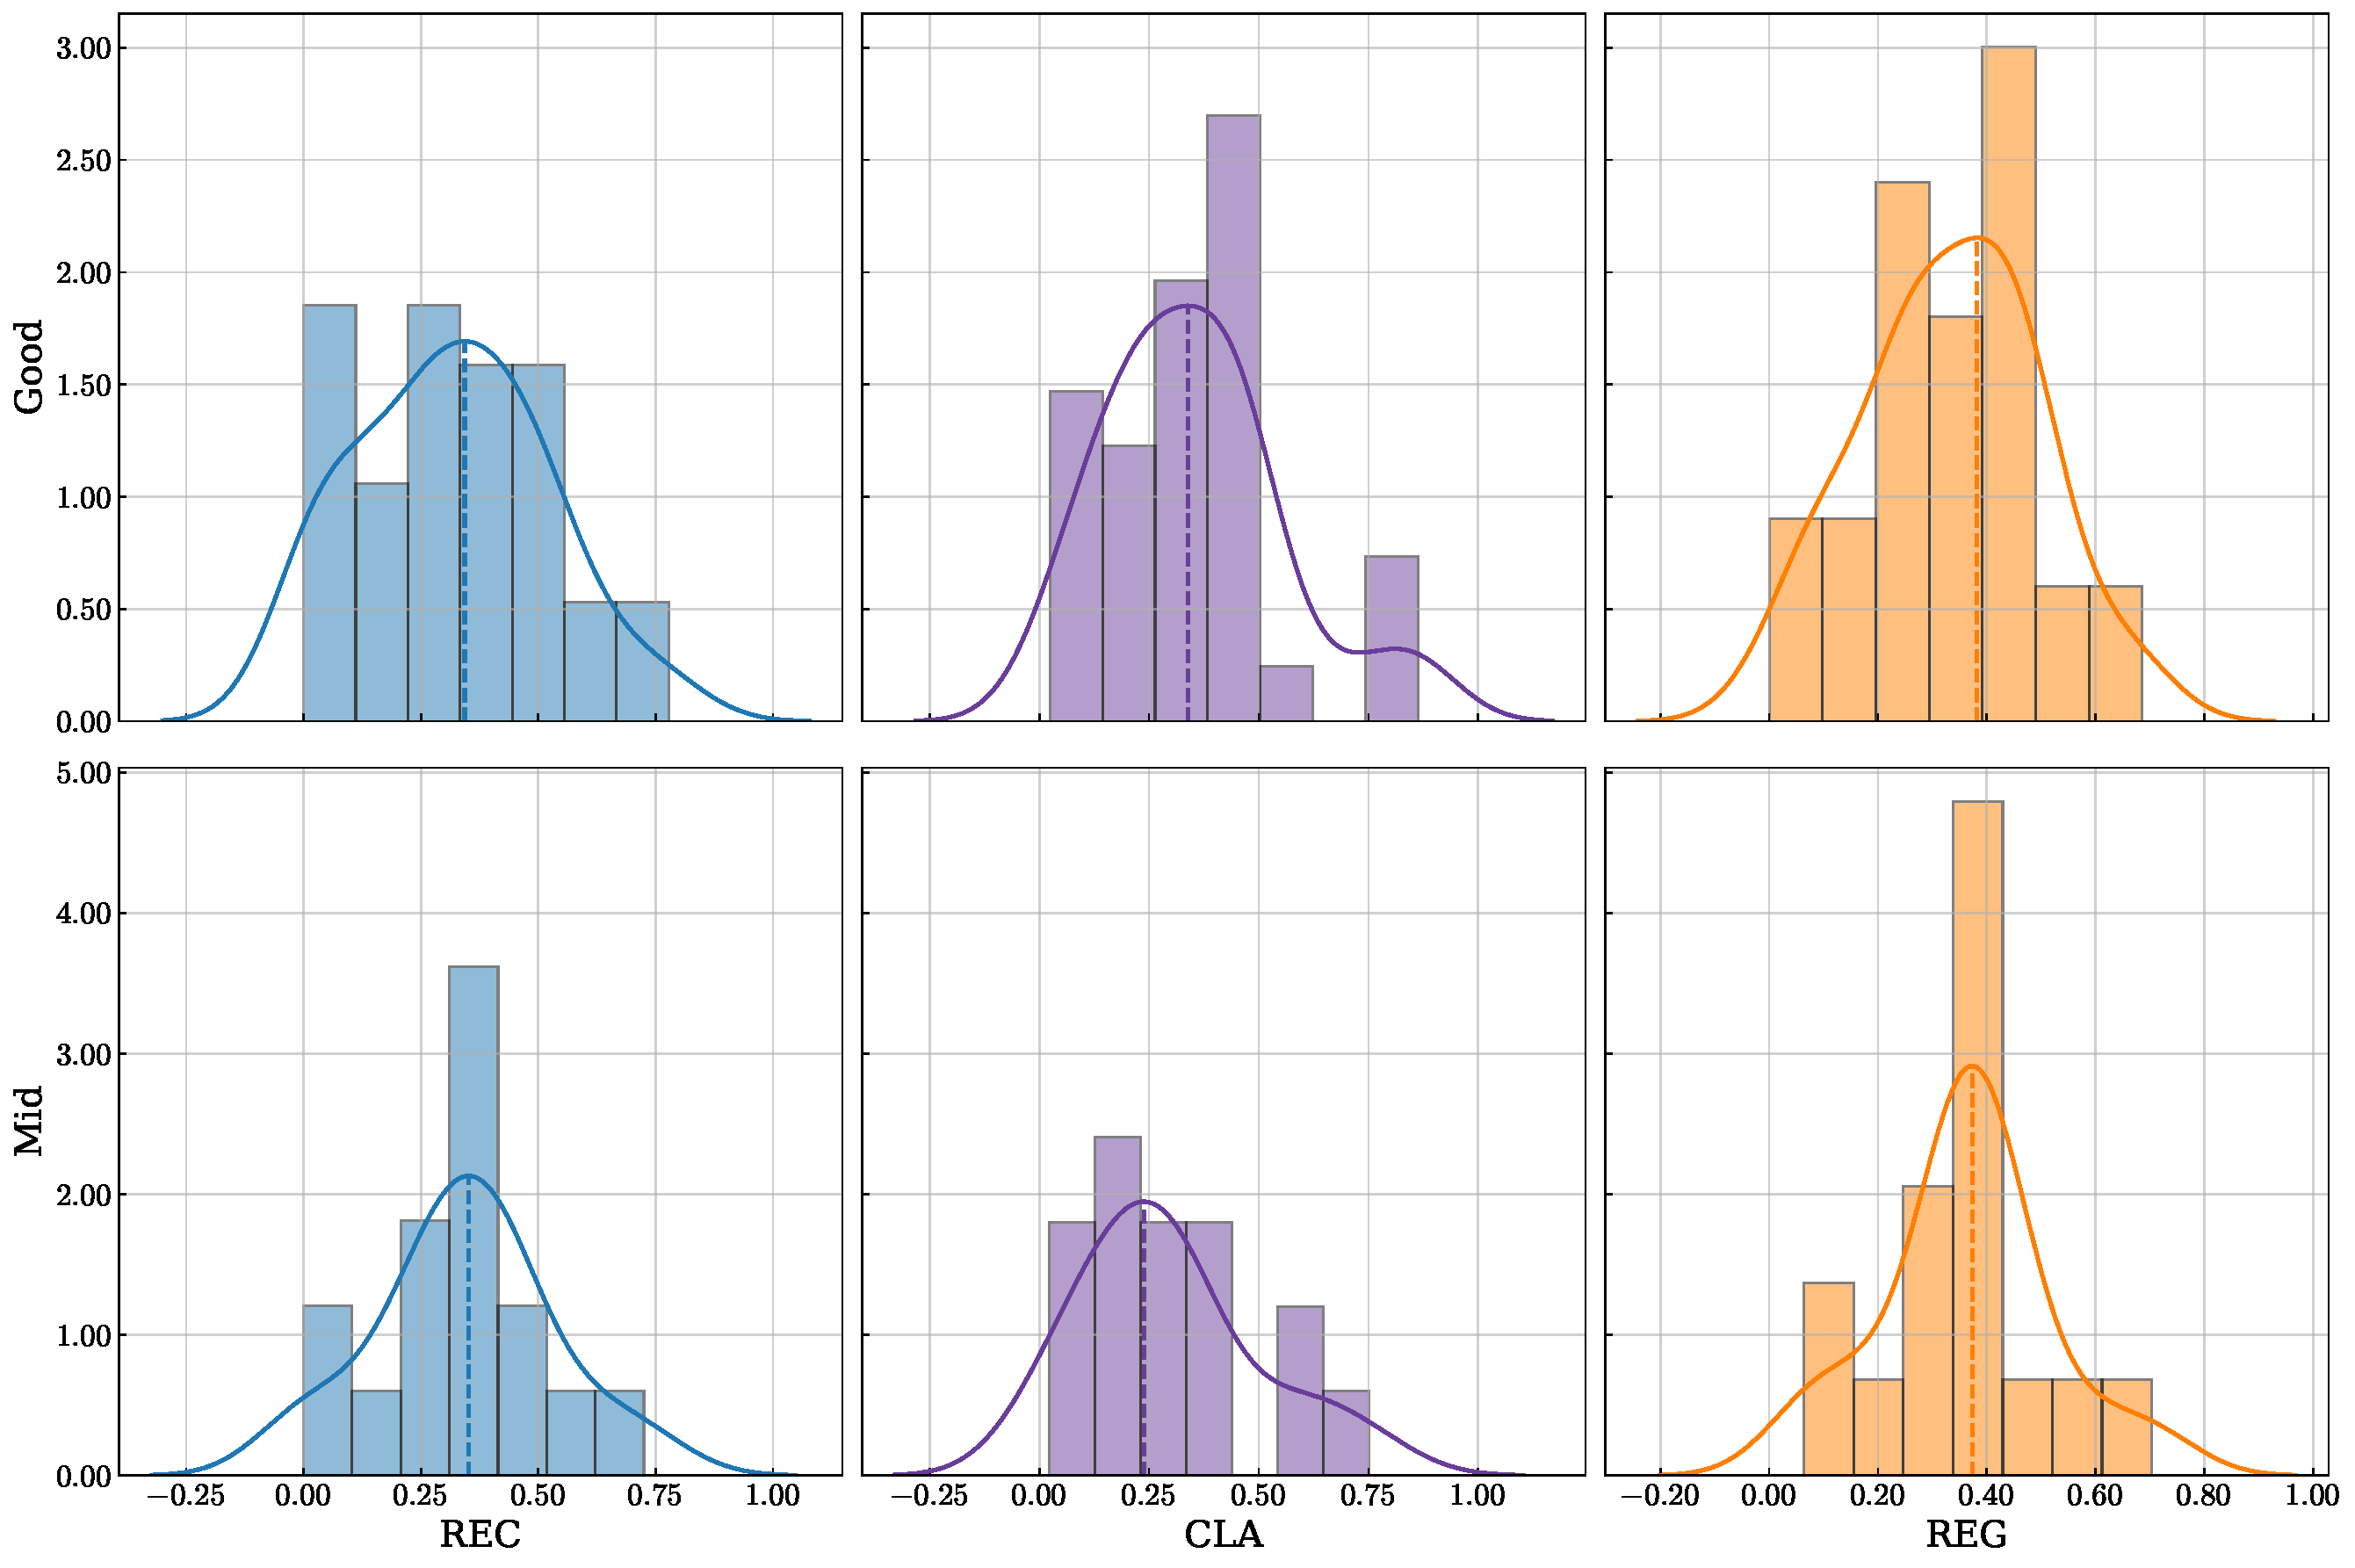
\includegraphics[width=\linewidth]{Figures/distributions_histogram_mid_good_with_mode.pdf}
    \caption{Distributions
 of the weights corresponding to the three loss components—reconstruction (REC), classification (CLA), and latent space regularization (REG)—for the performance groups ``Good'' and ``Mid''. Solid curves represent the density estimates, while dashed vertical lines indicate the mode of each distribution.}
    \label{fig:distributions}
\end{figure}
%------------------------------------------------
A key feature of \gls{eeggcirnet} is its ability to adapt its optimization priorities based on signal quality. The distributions of the three loss component weights, presented in Figure~\ref{fig:distributions}, reveal a distinct internal reorganization between the ``Good'' and ``Mid'' performance groups for the bi-class scenario. This behavior highlights the model’s inherent ability to promote a balanced interaction between reconstruction accuracy, discriminative capacity, and latent space stability. For the ``Good'' group, the weights for reconstruction (REC), classification (CLA), and latent space regularization (REG) are relatively balanced (modes: $0.3433$, $0.3390$, and $0.3824$, respectively). The slight predominance of the REG component suggests a focus on maintaining a coherent latent structure, which aligns with recent findings on the importance of regularization for robust performance~\cite{10483787}. 

In contrast, for the ``Mid'' group, the model distinctly reorganizes its priorities. The REG component remains dominant (mode: $0.3732$), but the CLA weight is significantly reduced (mode: $0.2382$) in favor of REC (mode: $0.3519$). This numerical shift, visible as a change in the central tendency of the distributions in Figure~\ref{fig:distributions}, indicates that when faced with less discriminative signals, the model prioritizes learning a stable and faithful representation of the input data over immediate classification accuracy. This adaptive strategy, where internal representation optimization substitutes for explicit discriminative signals, is a known characteristic of robust unimodal systems~\cite{Dhanushkodi}.
%---------------------------------------------------
%%% graficas hps Giga
%----------------------------------------------------
{To further examine the loss-weight reorganization, pairwise contour maps were built from the hyperparameter search of two representative subjects: Subject~14 from the ``Good'' group and Subject~27 from the ``Mid'' group. By visualizing the explored combinations of reconstruction (REC), classification (CLA), and regularization (REG) weights, these maps reveal how different optimization priorities shape the validation-accuracy landscape in \gls{eeggcirnet}.}

\begin{figure}[H]
\centering

\makebox[\textwidth][c]{%
\begin{minipage}[c]{0.99\textwidth}
\centering

\subfloat[REC vs. CLA]{%
    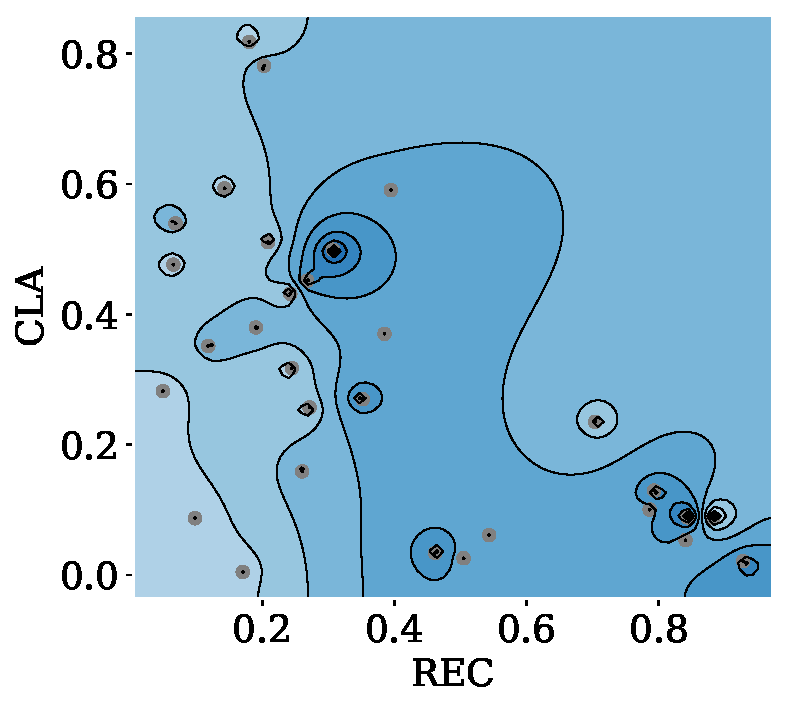
\includegraphics[width=0.34\linewidth,height=3.4cm]{Figures/contour_REC_vs_CLA-14.pdf}
}
\subfloat[REC vs. REG]{%
    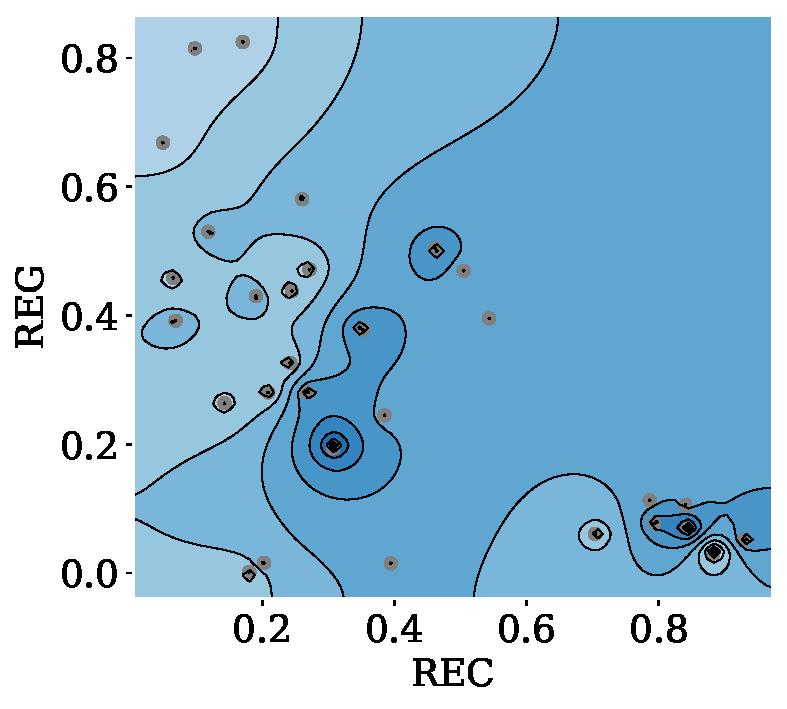
\includegraphics[width=0.34\linewidth,height=3.4cm]{Figures/contour_REC_vs_REG-14.pdf}
}
\subfloat[CLA vs. REG]{%
    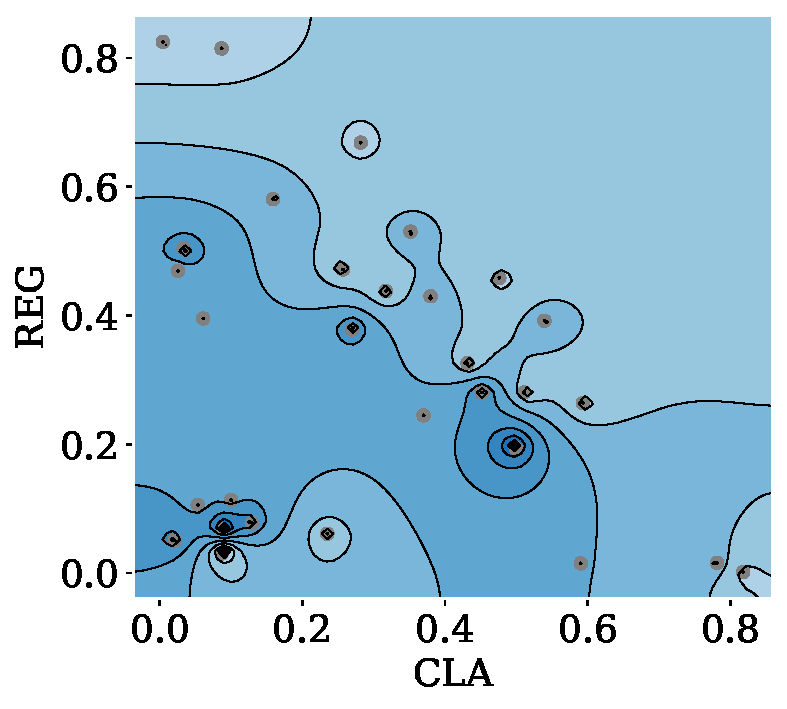
\includegraphics[width=0.34\linewidth,height=3.4cm]{Figures/contour_CLA_vs_REG-14.pdf}
}

\vspace{0.6em}

\begin{tikzpicture}
\begin{axis}[
    hide axis,
    scale only axis,
    width=\linewidth,
    height=0pt,
    colormap name=optunablues,
    colorbar horizontal,
    point meta min=88.4,
    point meta max=94,
    colorbar style={
        width=\linewidth,
        height=3mm,
        xtick={88.4, 89.2, 90, 90.8, 91.6, 92.4, 93.2, 94},
        xticklabel style={font=\scriptsize},
        xlabel={Val. accuracy (\%)},
        xlabel style={font=\scriptsize, yshift=2pt},
        scaled ticks=false,
        /pgf/number format/fixed,
        /pgf/number format/precision=1,
    },
]
\addplot [draw=none] coordinates {(0,0)};
\end{axis}
\end{tikzpicture}

\end{minipage}%
}

\caption{{Contour plots of validation accuracy (\%) as a function of the normalized loss weights REC, CLA, and REG for Subject~14, a representative subject from the ``Good'' group on the GigaScience dataset. All panels share the same color scale, allowing direct visual comparison across loss-weight pairs for this subject.}}
\label{fig:global_freq_GIGA14}
\end{figure}
%----------------------------------------------------
{For Subject~14 (Figure~\ref{fig:global_freq_GIGA14}), which is representative of the ``Good'' performance group, the contour maps reveal a broad and stable high-accuracy region across the explored loss-weight space. In all three pairwise projections, validation accuracy remains within a narrow high-performance range, indicating that the model is not strongly dependent on a single, highly specific combination of REC, CLA, and REG. This suggests that, for subjects with more discriminative EEG patterns, \gls{eeggcirnet} can preserve robust decoding performance under different optimization balances. The presence of extended high-accuracy regions rather than isolated optima indicates that reconstruction, classification, and latent-space regularization interact in a complementary manner, supporting representation stability and reducing abrupt performance degradation~\cite{10483787,Dhanushkodi}. This behavior is consistent with the balanced loss-weight distribution observed for the ``Good'' group in Figure~\ref{fig:distributions}, where the three components contribute relatively evenly to the optimization process.}

%----------------------------------------------------

\begin{figure}[H]
\centering

\makebox[\textwidth][c]{%
\begin{minipage}[c]{0.99\textwidth}
\centering

\subfloat[REC vs. CLA]{%
    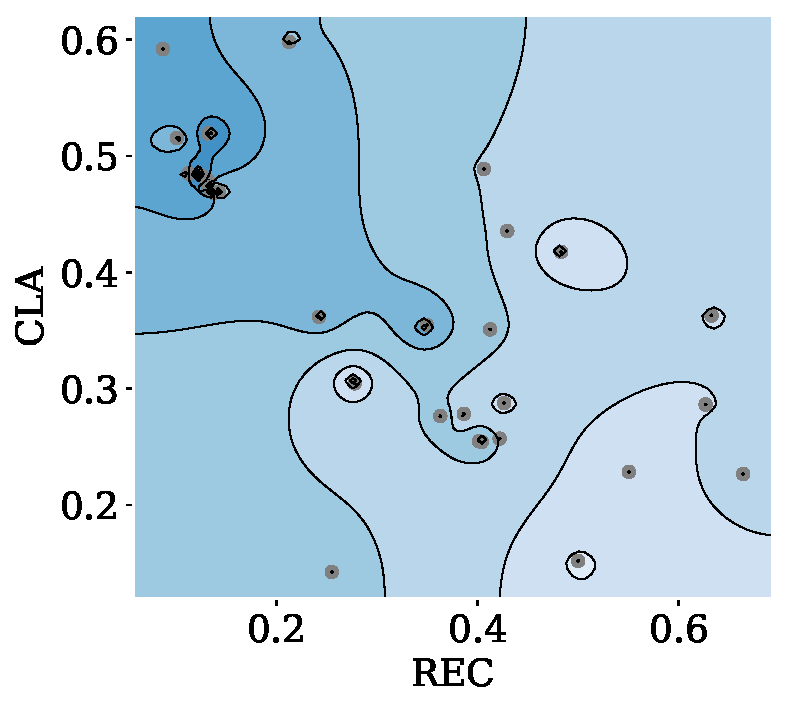
\includegraphics[width=0.34\linewidth,height=3.4cm]{Figures/contour_REC_vs_CLA-27.pdf}
}
\subfloat[REC vs. REG]{%
    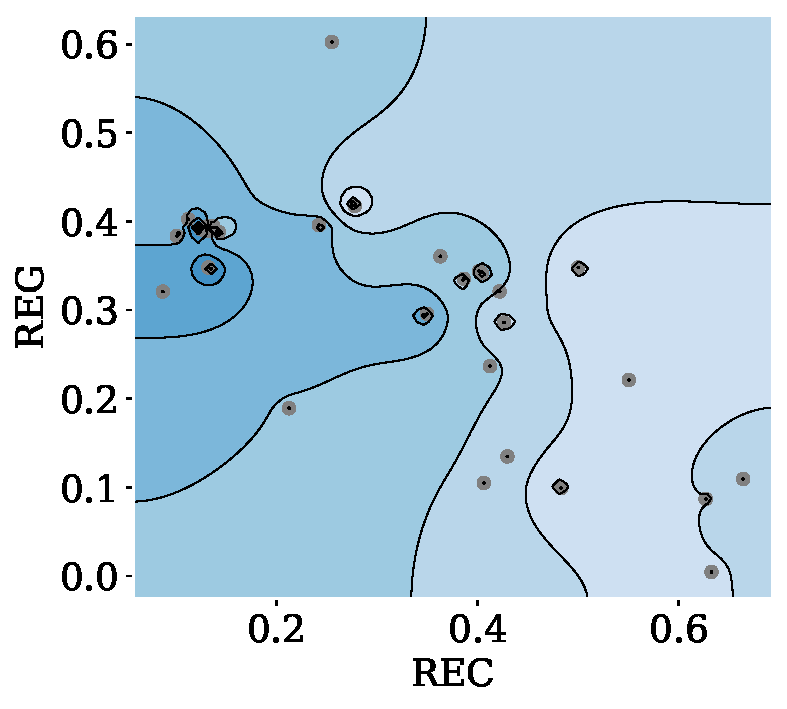
\includegraphics[width=0.34\linewidth,height=3.4cm]{Figures/contour_REC_vs_REG-27.pdf}
}
\subfloat[CLA vs. REG]{%
    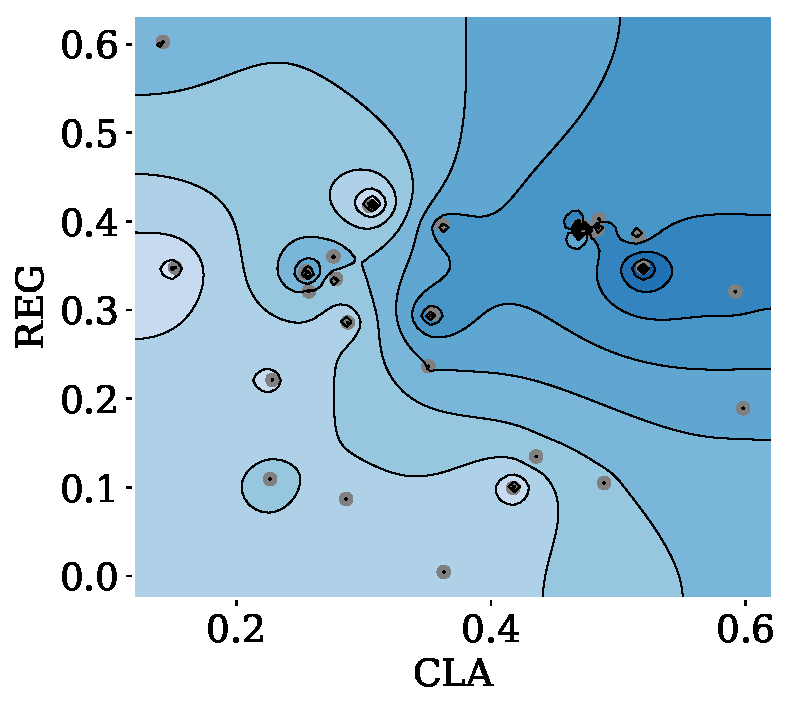
\includegraphics[width=0.34\linewidth,height=3.4cm]{Figures/contour_CLA_vs_REG-27.pdf}
}

\vspace{0.6em}

\begin{tikzpicture}
\begin{axis}[
    hide axis,
    scale only axis,
    width=\linewidth,
    height=0pt,
    colormap name=optunablues,
    colorbar horizontal,
    point meta min=51,
    point meta max=65,
    colorbar style={
        width=\linewidth,
        height=3mm,
        xtick={51, 53, 55, 57, 59, 61, 63, 65},
        xticklabel style={font=\scriptsize},
        xlabel={Val. accuracy (\%)},
        xlabel style={font=\scriptsize, yshift=2pt},
        scaled ticks=false,
        /pgf/number format/fixed,
        /pgf/number format/precision=1,
    },
]
\addplot [draw=none] coordinates {(0,0)};
\end{axis}
\end{tikzpicture}

\end{minipage}%
}

\caption{{Contour plots of validation accuracy (\%) as a function of the normalized loss weights REC, CLA, and REG for Subject~27, a representative subject from the ``Mid'' group on the GigaScience dataset. All panels share the same color scale, allowing direct visual comparison across loss-weight pairs for this subject.}}
\label{fig:global_freq_GIGA27}
\end{figure}
%----------------------------------------------------

{For Subject~27 (Figure~\ref{fig:global_freq_GIGA27}), representative of the ``Mid'' performance group, the validation-accuracy landscape is more heterogeneous than that observed for Subject~14. The lower and more variable accuracy range indicates that this subject is more sensitive to changes in the relative contribution of REC, CLA, and REG. Rather than exhibiting a broad region of stable high performance, the contour maps show more localized regions of improved validation accuracy, suggesting that adequate decoding depends on a more specific loss-weight configuration. This supports the idea that, under less discriminative EEG conditions, the model benefits from a stronger balance between faithful reconstruction and latent-space regularization to stabilize the learned representation~\cite{lotte2018review,saha2020intra}. This behavior agrees with Figure~\ref{fig:distributions}, where the ``Mid'' group shows a reduction in the CLA mode and a relative increase in REC and REG contributions.}

{After analyzing the loss-weight behavior at both the group level and in two representative subjects, we extended the analysis to the complete GigaScience dataset. For this purpose, the hyperparameter search records across all subjects were aggregated and analyzed using a global parameter-importance approach. This analysis estimates how much each optimized loss component contributed to explaining variations in validation accuracy across the full search space. Therefore, while Figures~\ref{fig:distributions},~\ref{fig:global_freq_GIGA14}, and~\ref{fig:global_freq_GIGA27} describe how the loss weights behave across groups and individual subjects, Figure~\ref{fig:GIGA_NRVAE} provides a population-level summary of the relative relevance of REC, CLA, and REG.}

\begin{figure}
    \centering
    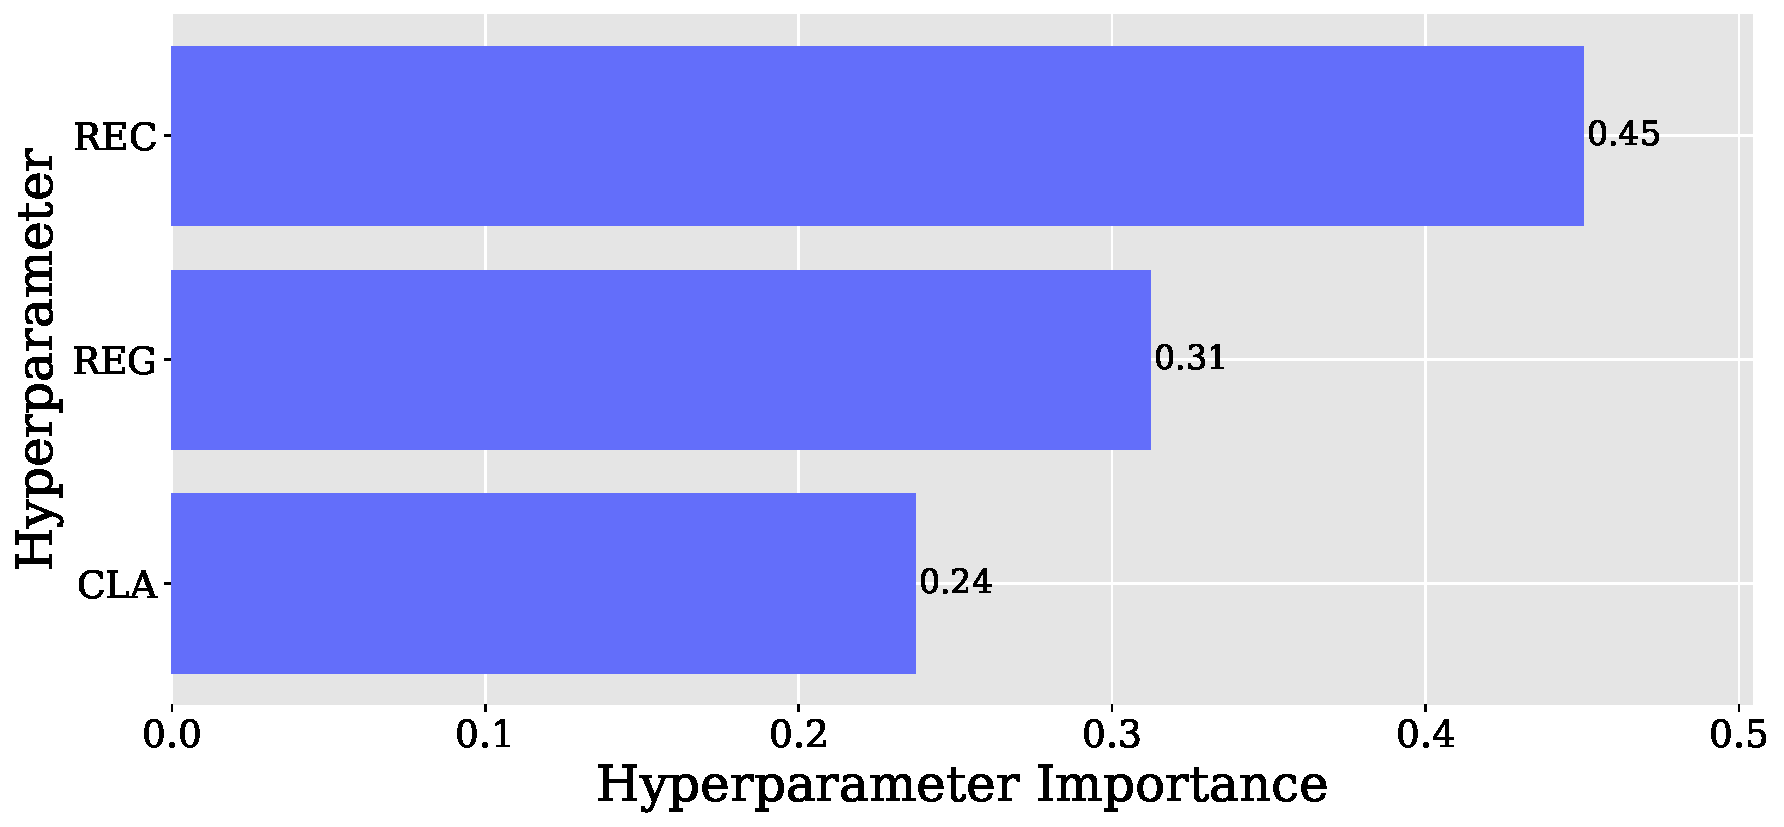
\includegraphics[width=0.8\linewidth]{Figures/optuna_fanova_param_importances_custom.pdf}
    \caption{{Global hyperparameter importance obtained from the Keras Tuner search history for the NRVAE loss-weight configuration across all GigaScience subjects. The importance scores quantify the relative contribution of REC, REG, and CLA to validation accuracy.}}
\label{fig:GIGA_NRVAE}
\end{figure}
%----------------------------------------------------
{The global importance analysis in Figure~\ref{fig:GIGA_NRVAE} shows that REC is the most influential loss-weight hyperparameter, with an importance score of $0.45$, followed by REG ($0.31$) and CLA ($0.24$). This result reinforces the interpretation that \gls{eeggcirnet} does not rely exclusively on direct discriminative optimization. Instead, validation performance across the GigaScience dataset is primarily shaped by the model's ability to preserve a faithful reconstruction of the input connectivity representation, while latent-space regularization provides an additional stabilizing effect~\cite{10483787,Dhanushkodi}. The lower, but still relevant, contribution of CLA indicates that classification remains necessary, but its effectiveness depends on the quality and stability of the learned representation. This finding is consistent with the previous group-level analysis, where the ``Mid'' group showed a reduction in CLA and a relative increase in REC and REG, suggesting that representation learning plays a central role in maintaining performance under more challenging EEG conditions, where inter-subject variability and nonstationarity commonly affect generalization~\cite{lotte2018review,saha2020intra}.}

%---------------------------------------------------
\begin{table}[H]
    \centering
    \caption{Subject-wise Bayesian-optimized loss weights and validation accuracy for \gls{eeggcirnet} on the BCI Competition IV-2a dataset, sorted according to validation performance.}
    \label{tab:bci2a_eegcirnet_hps}
    \begin{tabularx}{\textwidth}{CCCCC}
        \toprule
        \textbf{Subject} & \textbf{REC} & \textbf{CLA} & \textbf{REG} & \textbf{ACC [\%]} \\
        \midrule
        9 & $0.1074$ & $0.2713$ & $0.6213$ & $100.00$ \\
        
        8 & $0.2097$ & $0.2803$ & $0.5100$ & $100.00$ \\
        
        1 & $0.8701$ & $0.0636$ & $0.0663$ & $92.86$ \\
        
        3 & $0.4084$ & $0.0604$ & $0.5312$ & $91.07$ \\
        
        6 & $0.3381$ & $0.3358$ & $0.3261$ & $89.13$ \\
        
        7 & $0.0010$ & $0.5547$ & $0.4442$ & $83.33$ \\
        
        4 & $0.1464$ & $0.4641$ & $0.3895$ & $82.69$ \\
        
        5 & $0.1528$ & $0.3384$ & $0.5088$ & $80.77$ \\
        
        2 & $0.2166$ & $0.3495$ & $0.4340$ & $73.21$ \\
        \midrule
        \textbf{Average} &  & & & $\mathbf{88.56}$ \\
        \bottomrule
    \end{tabularx}
\end{table}
%---------------------------------------------------

%bci 2a 2 class
A complementary perspective on this adaptive behavior is observed in the canonical binary scenario of the BCI Competition IV-2a dataset, summarized in Table~\ref{tab:bci2a_eegcirnet_hps}. Unlike the multi-class \gls{eegmmidb} task or the subject-group validation protocol used for the \gls{adhd}/control dataset, this setting provides a more controlled and well-structured environment in which inter-class separability is generally higher and decision boundaries are more stable. Even under these favorable conditions, \gls{eeggcirnet} does not converge to a single fixed optimization regime, but instead exhibits subject-specific reweighting strategies that reflect the heterogeneity of neural patterns across individuals, a persistent challenge in \gls{eeg}-based \gls{bci} systems~\cite{lotte2018review,saha2020intra}.

For the highest-performing subjects (e.g., Subjects~8 and~9), the optimization converges toward a dominant regularization regime, with the latent regularization (REG) term exceeding $0.50$ and classification weights remaining moderate. This behavior indicates that, when discriminative patterns are highly consistent, enforcing a well-structured latent space becomes sufficient to sustain near-perfect classification performance, effectively stabilizing the learned representations without overemphasizing the discriminative loss. This interpretation is consistent with previous evidence indicating that latent-space regularization can improve robustness and reduce performance degradation in deep \gls{eeg} decoding models~\cite{10483787,Dhanushkodi}.

A more nuanced behavior emerges for subjects with high but non-saturated performance, confirming the presence of distinct subject-specific optimization strategies. Subject~1 exhibits a reconstruction-dominated regime, with REC receiving a markedly high weight ($0.8701$), while CLA and REG remain weakly weighted. This configuration suggests that, for this subject, accurate signal reconstruction plays a central role in preserving and structuring the \gls{eeg} representation prior to classification, in line with generative representation-learning approaches that use reconstruction to promote robust feature encoding~\cite{Dhanushkodi}. Subject~3 follows a hybrid strategy in which regularization and reconstruction dominate (REG $=0.5312$, REC $=0.4084$), while the classification component is strongly downweighted (CLA $=0.0604$). This indicates that stabilizing the latent structure is more critical than direct discriminative pressure for this individual. In contrast, Subject~6 displays a nearly uniform allocation across REC, CLA, and REG (REC $=0.3381$, CLA $=0.3358$, REG $=0.3261$), reflecting a balanced multi-objective optimization regime in which reconstruction fidelity, discriminative supervision, and latent stability jointly contribute to robust decoding.

For the remaining subjects with lower relative validation performance (e.g., Subjects~2,~4,~5, and~7), the optimization shifts toward increased emphasis on classification and latent regularization, with REC receiving comparatively less weight. This pattern suggests that, when signal quality or class separability is reduced, \gls{eeggcirnet} prioritizes strengthening discriminative supervision while simultaneously constraining the latent space to prevent overfitting. Such behavior mirrors the adaptive strategies observed in the ``Mid'' performance group of the GigaScience dataset and in more challenging subjects from the \gls{eegmmidb} collection, reinforcing the interpretation that reconstruction-driven representation learning and regularization act as complementary stabilizing mechanisms when discriminative cues alone are insufficient~\cite{10483787,Dhanushkodi}.

%----------contours---------------
{To further support this subject-specific interpretation, we analyzed the validation-accuracy landscapes obtained from the normalized loss-weight search for two representative cases of the BCI Competition IV-2a dataset: Subject~9, corresponding to the highest-performing subject, and Subject~2, corresponding to the lowest-performing subject. This comparison allows us to examine how the optimization landscape changes between a favorable decoding scenario and a more challenging subject-specific condition. The contour plots in Figures~\ref{fig:global_freq_9} and~\ref{fig:global_freq_2} show pairwise projections of the validation accuracy as a function of REC, CLA, and REG.}

%----------------------------------------------------
\begin{figure}[H]
\centering

\makebox[\textwidth][c]{%
\begin{minipage}[c]{0.99\textwidth}
\centering

\subfloat[REC vs. CLA]{%
    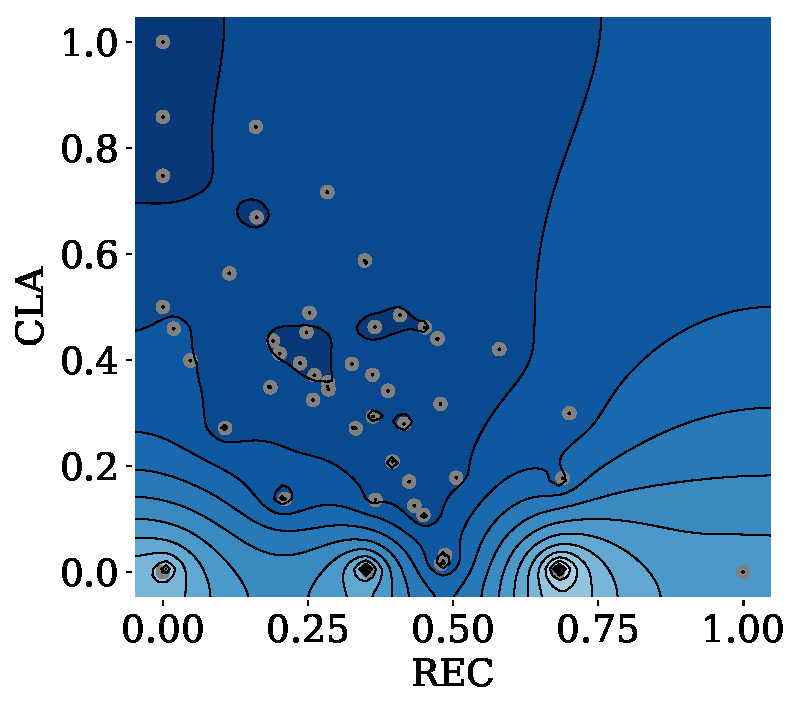
\includegraphics[width=0.34\linewidth,height=3.4cm]{Figures/contour_REC_vs_CLA-9.pdf}
}
\subfloat[REC vs. REG]{%
    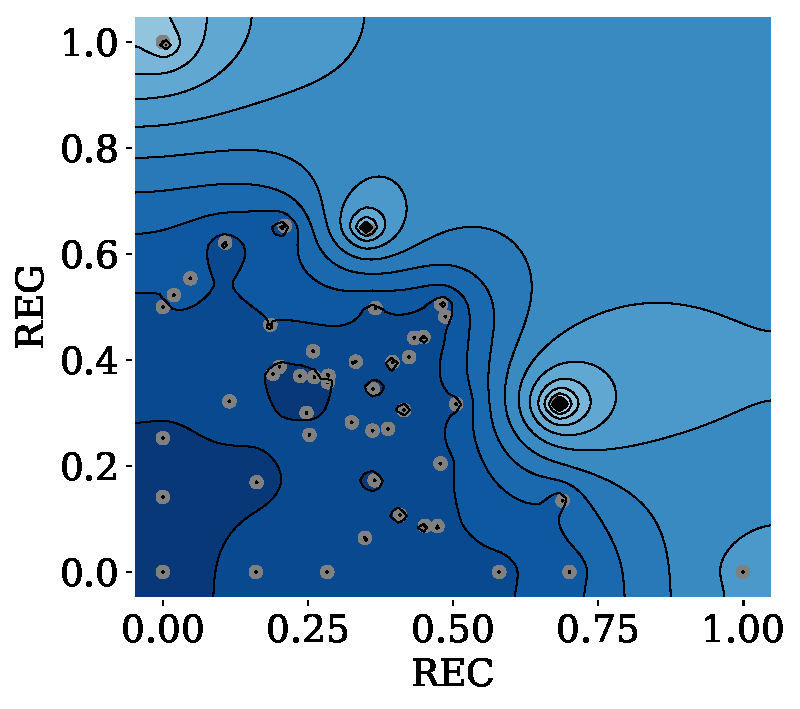
\includegraphics[width=0.34\linewidth,height=3.4cm]{Figures/contour_REC_vs_REG-9.pdf}
}
\subfloat[CLA vs. REG]{%
    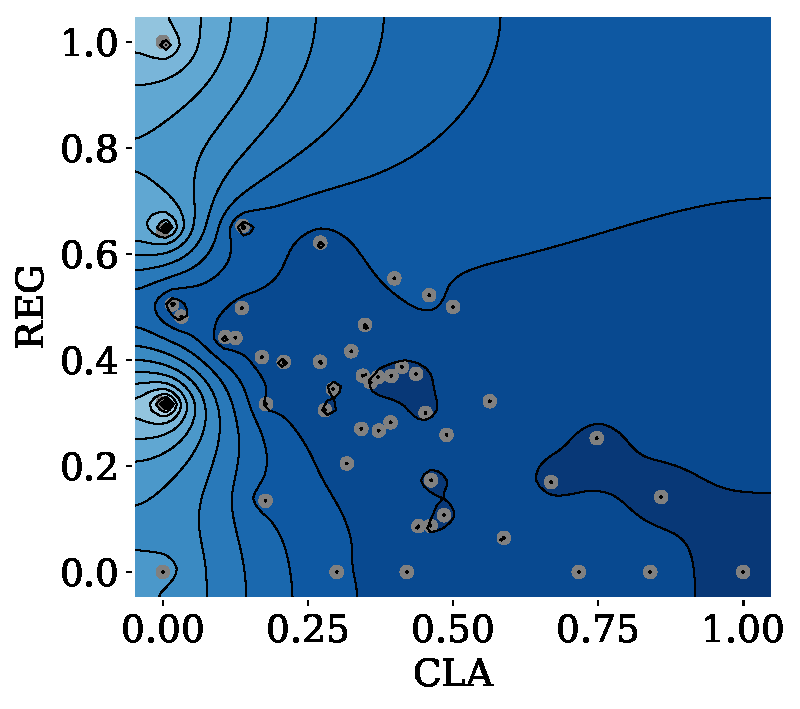
\includegraphics[width=0.34\linewidth,height=3.4cm]{Figures/contour_CLA_vs_REG-9.pdf}
}

\vspace{0.6em}

\begin{tikzpicture}
\begin{axis}[
    hide axis,
    scale only axis,
    width=\linewidth,
    height=0pt,
    colormap name=optunablues,
    colorbar horizontal,
    point meta min=54,
    point meta max=100,
    colorbar style={
        width=\linewidth,
        height=3mm,
        xtick={54, 60, 66, 72, 78, 84, 90, 96, 100},
        xticklabel style={font=\scriptsize},
        xlabel={Val. accuracy (\%)},
        xlabel style={font=\scriptsize, yshift=2pt},
        scaled ticks=false,
        /pgf/number format/fixed,
        /pgf/number format/precision=1,
    },
]
\addplot [draw=none] coordinates {(0,0)};
\end{axis}
\end{tikzpicture}

\end{minipage}%
}

\caption{{Contour plots of validation accuracy (\%) as a function of the normalized loss weights REC, CLA, and REG for Subject~9, the highest-performing subject on the BCI Competition IV-2a dataset. All panels share the same color scale, allowing direct visual comparison across loss-weight pairs for this subject.}}
\label{fig:global_freq_9}
\end{figure}

%----------------------------------------------------
{For Subject~9 (Figure~\ref{fig:global_freq_9}), the contour maps show extended high-performance regions across the explored loss-weight space. This behavior indicates that, for this highly discriminative subject, \gls{eeggcirnet} is relatively robust to moderate variations in the balance among REC, CLA, and REG. In particular, the validation landscape suggests that high accuracy can be preserved across several configurations, provided that the latent representation remains sufficiently structured and the classification term maintains a non-negligible contribution. This agrees with the optimized weights reported in Table~\ref{tab:bci2a_eegcirnet_hps}, where Subject~9 achieves $100\%$ validation accuracy with a REG-dominated configuration. Therefore, in favorable decoding conditions, latent-space regularization appears to act as a stabilizing mechanism that supports near-perfect performance without requiring an excessively dominant classification loss~\cite{10483787,Dhanushkodi}.}

%--------------------------------
\begin{figure}[H]
\centering

\makebox[\textwidth][c]{%
\begin{minipage}[c]{0.99\textwidth}
\centering

\subfloat[REC vs. CLA]{%
    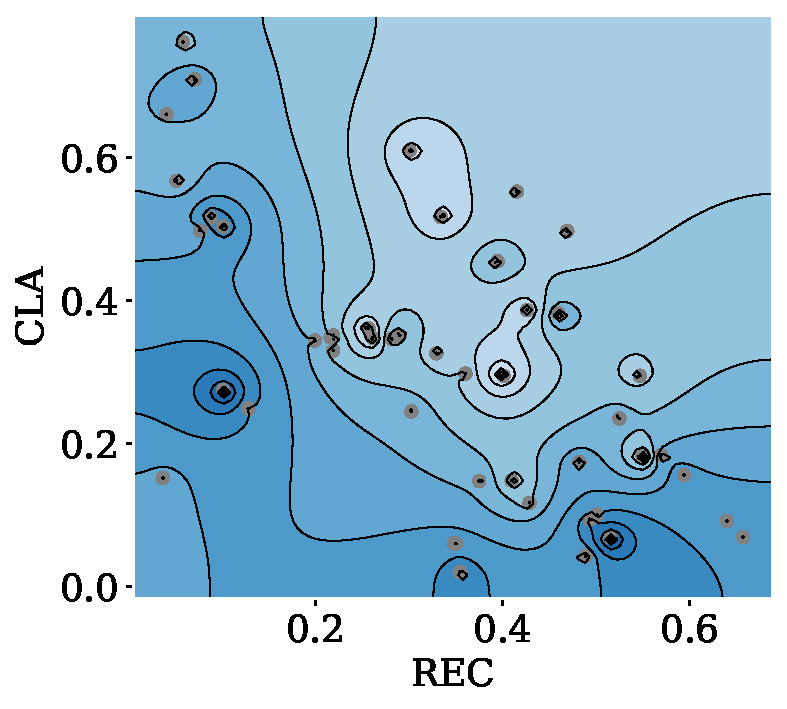
\includegraphics[width=0.34\linewidth,height=3.4cm]{Figures/contour_REC_vs_CLA-2.pdf}
}
\subfloat[REC vs. REG]{%
    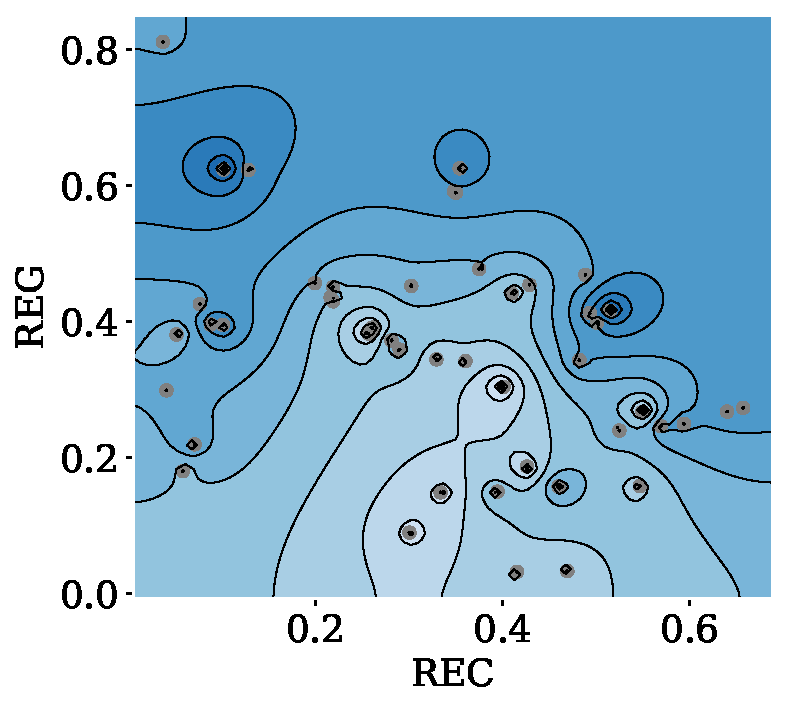
\includegraphics[width=0.34\linewidth,height=3.4cm]{Figures/contour_REC_vs_REG-2.pdf}
}
\subfloat[CLA vs. REG]{%
    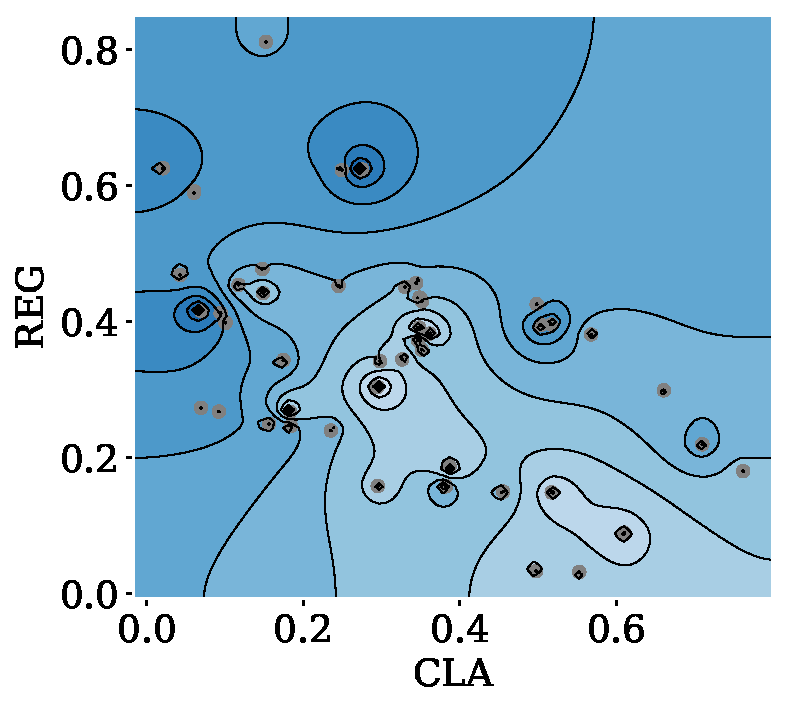
\includegraphics[width=0.34\linewidth,height=3.4cm]{Figures/contour_CLA_vs_REG-2.pdf}
}

\vspace{0.6em}

\begin{tikzpicture}
\begin{axis}[
    hide axis,
    scale only axis,
    width=\linewidth,
    height=0pt,
    colormap name=optunablues,
    colorbar horizontal,
    point meta min=58,
    point meta max=74,
    colorbar style={
        width=\linewidth,
        height=3mm,
        xtick={58, 60, 62, 64, 66, 68, 70, 72, 74},
        xticklabel style={font=\scriptsize},
        xlabel={Val. accuracy (\%)},
        xlabel style={font=\scriptsize, yshift=2pt},
        scaled ticks=false,
        /pgf/number format/fixed,
        /pgf/number format/precision=1,
    },
]
\addplot [draw=none] coordinates {(0,0)};
\end{axis}
\end{tikzpicture}

\end{minipage}%
}

\caption{{Contour plots of validation accuracy (\%) as a function of the normalized loss weights REC, CLA, and REG for Subject~2, the lowest-performing subject on the BCI Competition IV-2a dataset. All panels share the same color scale, allowing direct visual comparison across loss-weight pairs for this subject.}}
\label{fig:global_freq_2}
\end{figure}

%-------------------------------------------------------
{For Subject~2 (Figure~\ref{fig:global_freq_2}), which corresponds to the lowest-performing subject in the BCI Competition IV-2a analysis, the validation-accuracy landscape is more restricted and heterogeneous than that observed for Subject~9. The lower accuracy range and the presence of localized high-performance regions indicate that this subject is more sensitive to the precise balance among REC, CLA, and REG. In particular, the contour maps suggest that improved validation performance is not achieved across broad regions of the search space, but rather within narrower configurations where discriminative supervision and latent-space regularization remain sufficiently emphasized. This interpretation is consistent with the optimized weights reported in Table~\ref{tab:bci2a_eegcirnet_hps}, where Subject~2 reaches its best performance with a combined contribution of REG ($0.4340$) and CLA ($0.3495$), while REC receives a comparatively lower weight ($0.2166$). These results suggest that, under more challenging subject-specific conditions, \gls{eeggcirnet} relies more strongly on classification guidance and latent-space constraints to stabilize the learned representation and prevent performance degradation. This behavior is consistent with the known impact of inter-subject variability on \gls{eeg}-based \gls{bci} generalization~\cite{lotte2018review,saha2020intra}.}

{After examining the subject-specific contour maps, we performed a global hyperparameter-importance analysis across all subjects of the BCI Competition IV-2a dataset. This analysis summarizes the relative contribution of the reconstruction (REC), classification (CLA), and latent-space regularization (REG) weights to validation accuracy, providing a dataset-level view of which loss components most strongly influenced the optimization of \gls{eeggcirnet}.}
%-------------------------------------------------------

\begin{figure}[H]
    \centering
    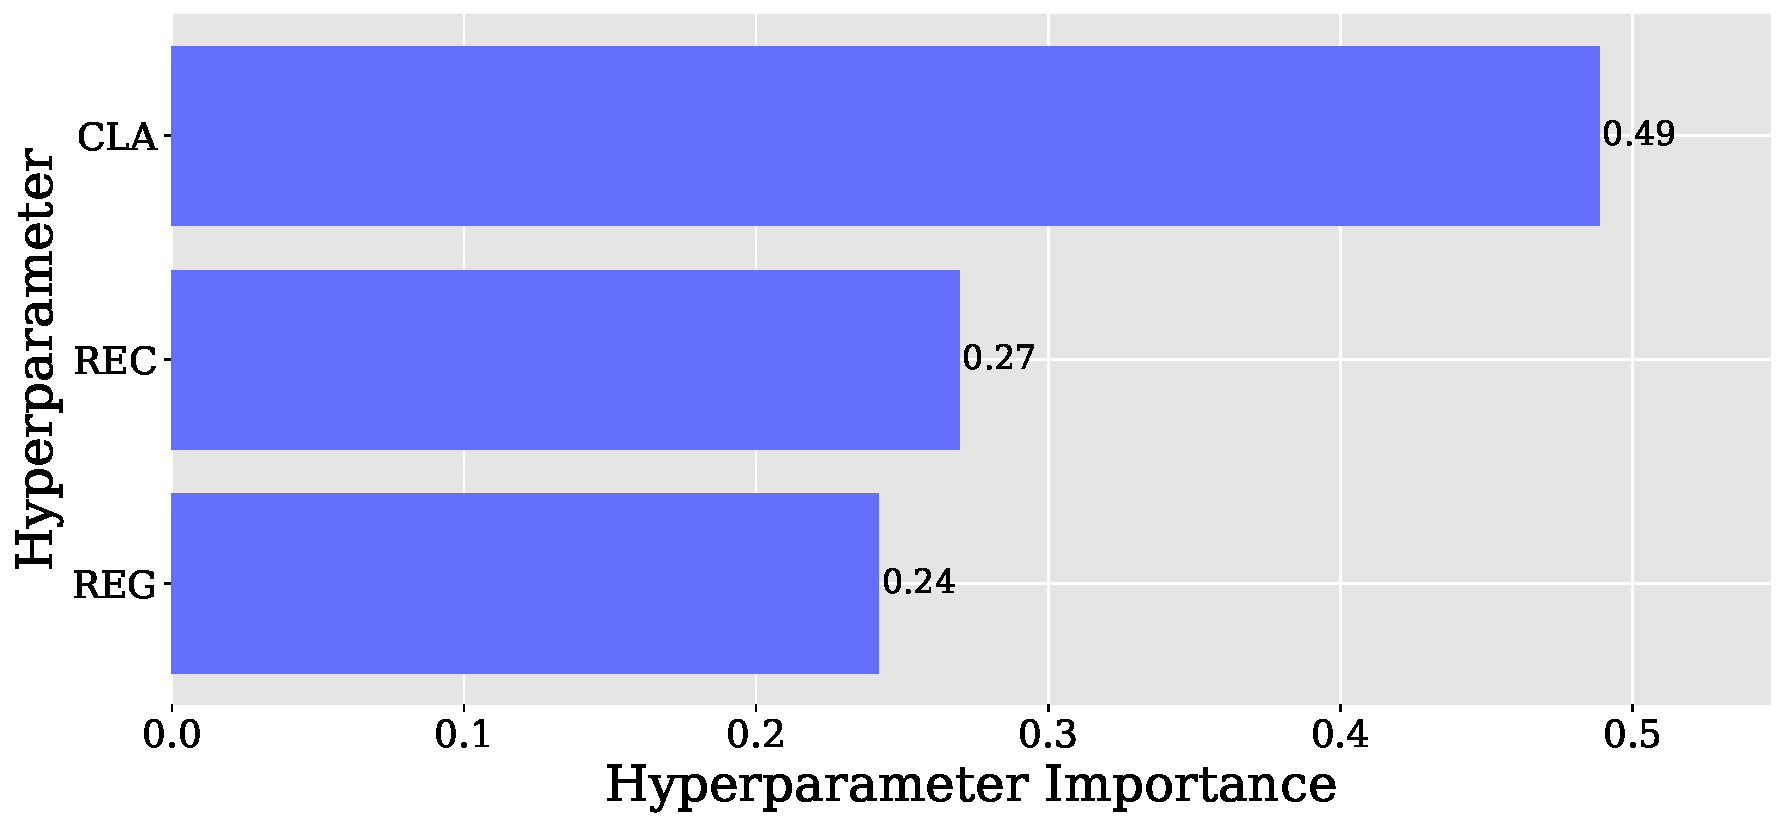
\includegraphics[width=0.8\linewidth]{Figures/optuna_fanova_param_importances_BCI2A-_NRVAE.pdf}
    \caption{{Global hyperparameter importance of the optimized \gls{eeggcirnet} loss weights on the BCI Competition IV-2a dataset. The importance scores quantify the relative contribution of reconstruction (REC), classification (CLA), and latent-space regularization (REG) weights to validation accuracy.}}
    \label{fig:bci2a_fanova_importance}
\end{figure}

%-------------------------------------------------------

{The global importance analysis in Figure~\ref{fig:bci2a_fanova_importance} shows that CLA is the most influential loss-weight hyperparameter in the BCI Competition IV-2a scenario, with an importance score of $0.49$, followed by REC ($0.27$) and REG ($0.24$). This result contrasts with the GigaScience analysis, where REC had the largest global contribution, and suggests that the canonical binary BCI IV-2a setting relies more strongly on direct discriminative supervision. Nevertheless, the non-negligible contributions of REC and REG indicate that classification performance is still supported by representation reconstruction and latent-space stabilization. Therefore, even in a more controlled binary decoding task, \gls{eeggcirnet} benefits from a multi-objective optimization strategy rather than relying exclusively on the classification loss. This finding reinforces the role of adaptive loss-weight reorganization as a mechanism for balancing discriminative learning with representation stability under subject-specific \gls{eeg} variability~\cite{lotte2018review,saha2020intra,Dhanushkodi}.}

Taken together, the BCI Competition IV-2a results complete the picture established across datasets: \gls{eeggcirnet} does not rely on a fixed balance between reconstruction, classification, and regularization, but dynamically reorganizes its internal optimization priorities according to signal characteristics and task difficulty. This consistency across canonical, multi-class, and subject-group validation scenarios provides strong evidence that the proposed framework internalizes a principled adaptive learning strategy rather than overfitting to any particular experimental condition, addressing a central limitation of \gls{eeg}-based \gls{bci} models under inter-subject variability~\cite{lotte2018review,saha2020intra}.

%----------------------------------------------------
%%aqui quedeeeeeeeee
%----------------------------------------------------

%physionet
\begin{table}[H]
    \centering
    \caption{Subject-specific weight distribution for reconstruction (REC), classification (CLA), latent regularization (REG), and mean accuracy across the selected subjects of the \gls{eegmmidb} dataset.}
    \label{tab:weights_dist}
    \begin{tabularx}{\textwidth}{CCCCC}
        \toprule
        \textbf{Subject} & \textbf{REC} & \textbf{CLA} & \textbf{REG} & \textbf{ACC [\%]} \\
        \midrule
        $13$ & $0.0000$ & $1.0000$ & $0.0000$ & $77.80$ \\
        $50$ & $0.5000$ & $0.5000$ & $0.0000$ & $77.76$ \\
        $12$ & $0.3655$ & $0.6345$ & $0.0000$ & $77.77$ \\
        $9$  & $0.3803$ & $0.6197$ & $0.0000$ & $76.19$ \\
        $40$ & $0.3559$ & $0.6441$ & $0.0000$ & $76.20$ \\
        $7$  & $0.4958$ & $0.3824$ & $0.1219$ & $77.70$ \\
        $41$ & $0.5401$ & $0.4583$ & $0.0017$ & $71.40$ \\
        $49$ & $0.8303$ & $0.1697$ & $0.0000$ & $73.00$ \\
        $3$  & $0.4421$ & $0.4615$ & $0.0964$ & $71.43$ \\
        $8$  & $0.3869$ & $0.4379$ & $0.1753$ & $73.02$ \\
        \midrule
        \textbf{Average} &  &  &  & $\mathbf{75.20}$ \\
        \bottomrule
    \end{tabularx}
\end{table}

%----------------------------------------------------
%physionet multiclass
Likewise, we analyzed the learned loss component weights ($\lambda_{\text{REC}}$, $\lambda_{\text{CLA}}$, $\lambda_{\text{REG}}$) for the multi-class scenario, as detailed in Table~\ref{tab:weights_dist}. The distribution of these weights corroborates the adaptive optimization strategy observed in the binary task, but reveals distinct behaviors necessitated by the increased complexity of the 5-class problem. For the highest-performing subject (Subject 13), the model converges to a purely discriminative state ($\lambda_{\text{CLA}} = 1.0000$, $\lambda_{\text{REC}} = \lambda_{\text{REG}} = 0$), indicating that the spatio-spectral features were sufficiently distinct to drive classification without the need for auxiliary regularization. Conversely, for subjects with moderate performance (e.g., S50, S12, S40), the model adopts a hybrid strategy, balancing classification importance ($\lambda_{\text{CLA}} \approx 0.60$) with reconstruction fidelity ($\lambda_{\text{REC}} \approx 0.40$), while keeping the latent regularization term deactivated ($\lambda_{\text{REG}} = 0$). This suggests that for reasonably separable data, the autoencoder acts primarily as a feature extractor rather than a generative regularizer.

However, a critical shift occurs for the most challenging subjects (e.g., 7, 3, 8), where the baseline methods struggled. Here, the model explicitly activates the latent space regularization ($\lambda_{\text{REG}} > 0.09$), reaching values up to $0.1753$ for Subject 8. This indicates that when decision boundaries are ambiguous, \gls{eeggcirnet} automatically prioritizes the formation of a well-structured Gaussian latent space to prevent overfitting. An extreme case is observed for Subject 49, where the model shifts almost entirely to representation learning ($\lambda_{\text{REC}} = 0.8303$), effectively operating as a non-linear denoiser to stabilize the input features before attempting classification. This evident reorganization of optimization priorities confirms that the architecture is not a static ``black box,'' but an adaptive system that modulates its learning objective based on the difficulty of the underlying \mbox{neural patterns.}

%----------contours EEGMMIDB---------------

{To further support the subject-specific interpretation derived from Table~\ref{tab:weights_dist}, we analyzed the validation-accuracy landscapes for two representative subjects from the multi-class \gls{eegmmidb} scenario: Subject~12, one of the highest-performing subjects, and Subject~41, a moderate-performance subject. This comparison provides a visual characterization of how the optimized balance among reconstruction (REC), classification (CLA), and latent-space regularization (REG) changes as the 5-class decoding problem becomes more challenging. The contour plots in Figures~\ref{fig:global_freq_12} and~\ref{fig:global_freq_Sbj41} show pairwise projections of the validation accuracy over the normalized loss-weight space.}

%----------------------------------------------------
\begin{figure}[htbp]]
\centering

\makebox[\textwidth][c]{%
\begin{minipage}[c]{0.99\textwidth}
\centering

\subfloat[REC vs. CLA]{%
    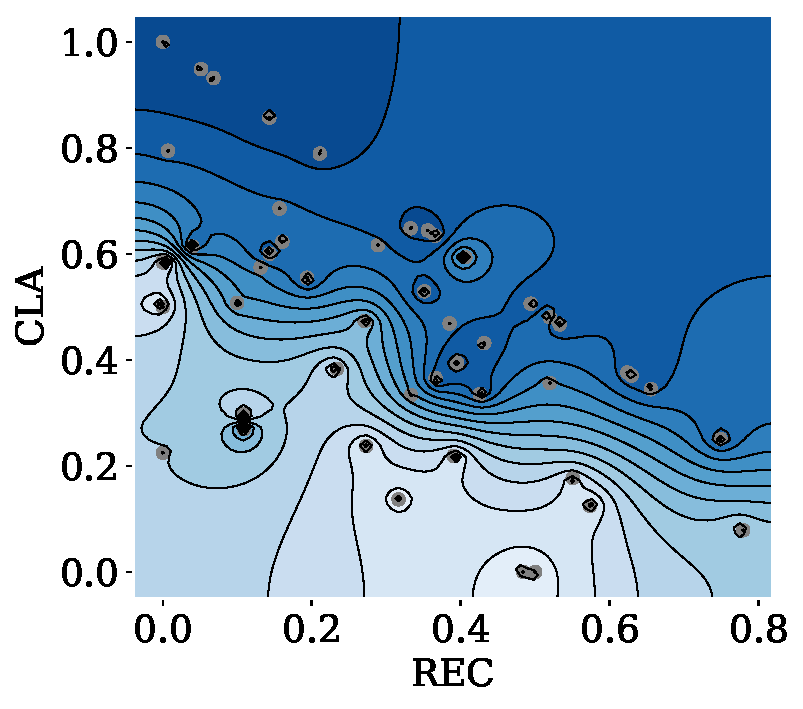
\includegraphics[width=0.34\linewidth,height=3.4cm]{Figures/contour_REC_vs_CLA-12.pdf}
}
\subfloat[REC vs. REG]{%
    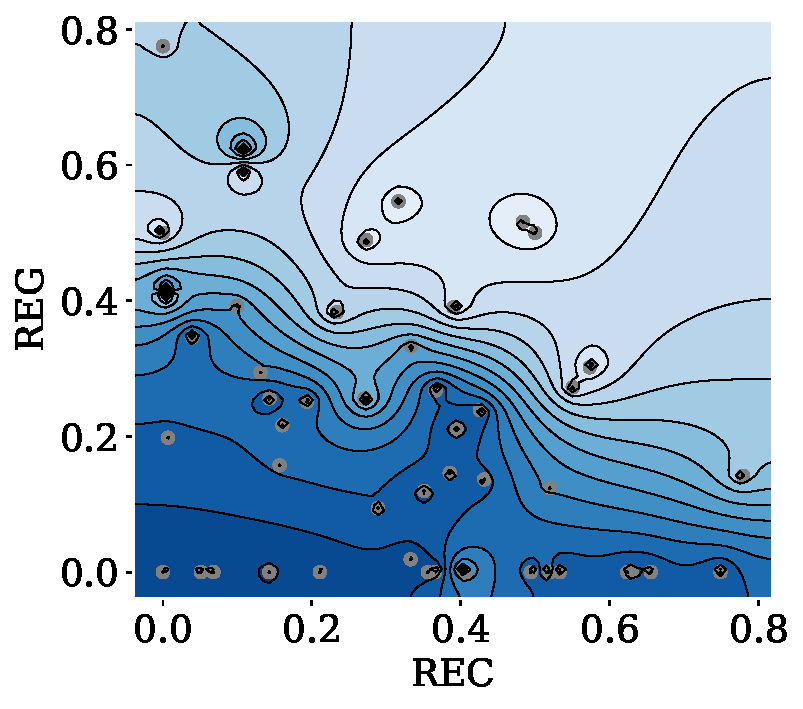
\includegraphics[width=0.34\linewidth,height=3.4cm]{Figures/contour_REC_vs_REG-12.pdf}
}
\subfloat[CLA vs. REG]{%
    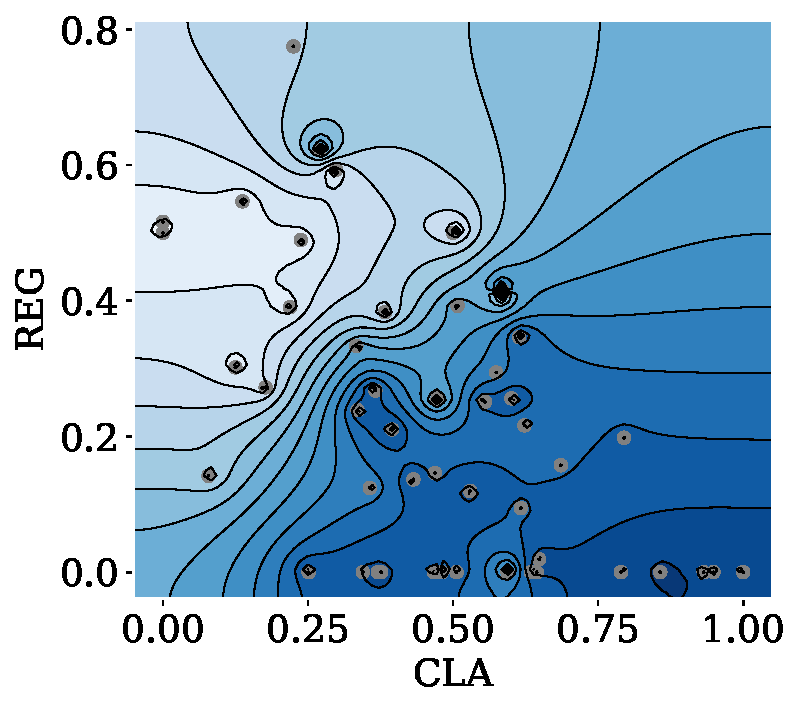
\includegraphics[width=0.34\linewidth,height=3.4cm]{Figures/contour_CLA_vs_REG-12.pdf}
}

\vspace{0.6em}

\begin{tikzpicture}
\begin{axis}[
    hide axis,
    scale only axis,
    width=\linewidth,
    height=0pt,
    colormap name=optunablues,
    colorbar horizontal,
    point meta min=20,
    point meta max=77,
    colorbar style={
        width=\linewidth,
        height=3mm,
        xtick={20, 28, 36, 44, 52, 60, 68, 77},
        xticklabel style={font=\scriptsize},
        xlabel={Val. accuracy (\%)},
        xlabel style={font=\scriptsize, yshift=2pt},
        scaled ticks=false,
        /pgf/number format/fixed,
        /pgf/number format/precision=1,
    },
]
\addplot [draw=none] coordinates {(0,0)};
\end{axis}
\end{tikzpicture}

\end{minipage}%
}

\caption{{Contour plots of validation accuracy (\%) as a function of the normalized loss weights REC, CLA, and REG for Subject~12, one of the highest-performing subjects in the \gls{eegmmidb} multi-class scenario. All panels share the same color scale, allowing direct visual comparison across loss-weight pairs for this subject.}}
\label{fig:global_freq_12}
\end{figure}
%----------------------------------------------------

{For Subject~12 (Figure~\ref{fig:global_freq_12}), the validation landscape shows extended high-performance regions mainly associated with a strong classification contribution and low latent regularization. This behavior agrees with the optimized weights reported in Table~\ref{tab:weights_dist}, where Subject~12 achieves high accuracy with a CLA-dominant configuration ($\lambda_{\text{CLA}}=0.6345$), a relevant reconstruction contribution ($\lambda_{\text{REC}}=0.3655$), and inactive regularization ($\lambda_{\text{REG}}=0$). Thus, for this favorable multi-class case, direct discriminative supervision appears to be the main optimization driver, while reconstruction still contributes to preserving a stable connectivity-based representation, consistent with representation-learning strategies where reconstruction supports robust feature encoding~\cite{Dhanushkodi}.}

%----------------------------------------------------
\begin{figure}[htbp]]
\centering

\makebox[\textwidth][c]{%
\begin{minipage}[c]{0.99\textwidth}
\centering

\subfloat[REC vs. CLA]{%
    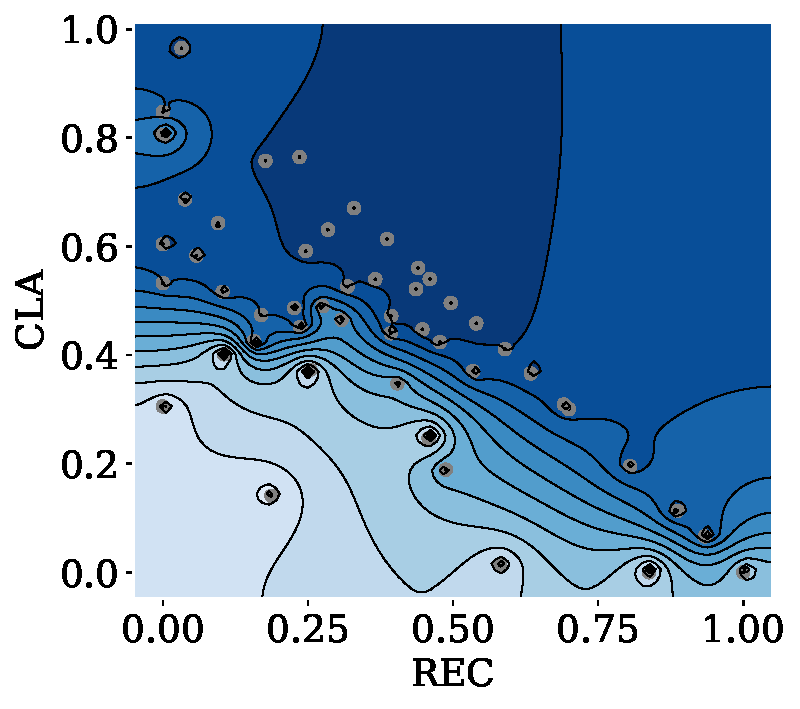
\includegraphics[width=0.34\linewidth,height=3.4cm]{Figures/contour_REC_vs_CLA-41.pdf}
}
\subfloat[REC vs. REG]{%
    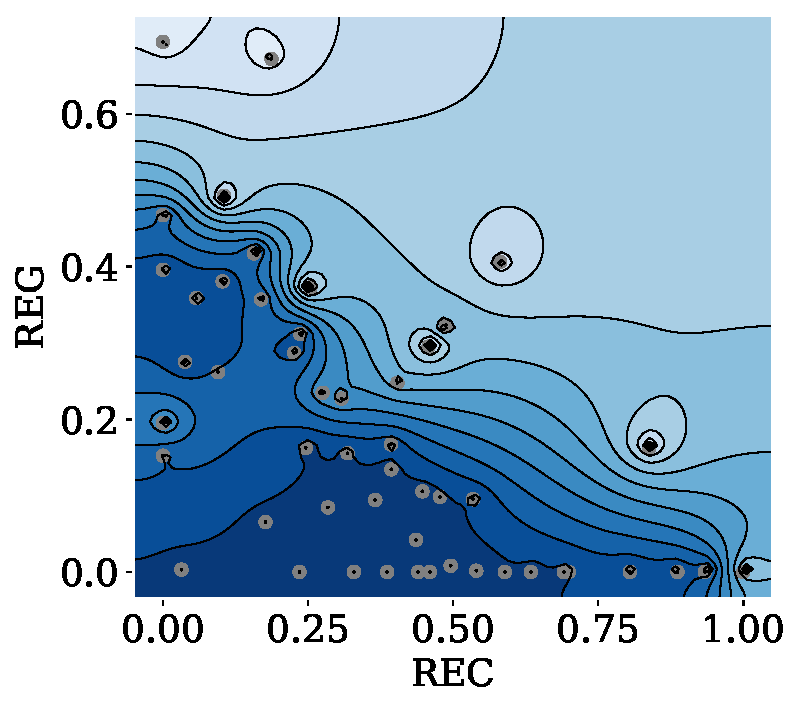
\includegraphics[width=0.34\linewidth,height=3.4cm]{Figures/contour_REC_vs_REG-41.pdf}
}
\subfloat[CLA vs. REG]{%
    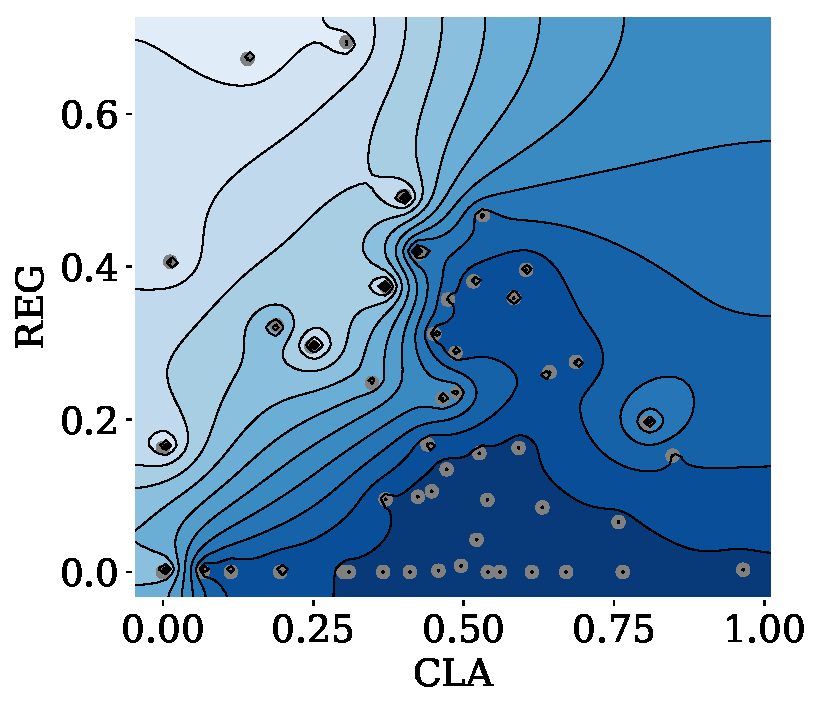
\includegraphics[width=0.34\linewidth,height=3.4cm]{Figures/contour_CLA_vs_REG-41.pdf}
}

\vspace{0.6em}

\begin{tikzpicture}
\begin{axis}[
    hide axis,
    scale only axis,
    width=\linewidth,
    height=0pt,
    colormap name=optunablues,
    colorbar horizontal,
    point meta min=20,
    point meta max=68,
    colorbar style={
        width=\linewidth,
        height=3mm,
        xtick={20, 28, 36, 44, 52, 60, 68},
        xticklabel style={font=\scriptsize},
        xlabel={Val. accuracy (\%)},
        xlabel style={font=\scriptsize, yshift=2pt},
        scaled ticks=false,
        /pgf/number format/fixed,
        /pgf/number format/precision=1,
    },
]
\addplot [draw=none] coordinates {(0,0)};
\end{axis}
\end{tikzpicture}

\end{minipage}%
}

\caption{{Contour plots of validation accuracy (\%) as a function of the normalized loss weights REC, CLA, and REG for Subject~41, a moderate-performance subject in the \gls{eegmmidb} multi-class scenario. All panels share the same color scale, allowing direct visual comparison across loss-weight pairs for this subject.}}
\label{fig:global_freq_Sbj41}
\end{figure}
%---------------------------------------------------

{For Subject~41 (Figure~\ref{fig:global_freq_Sbj41}), the contour maps reveal a more constrained validation landscape, suggesting greater sensitivity to the precise balance between reconstruction and classification. In contrast to Subject~12, the best-performing configuration for Subject~41 relies on a more balanced REC--CLA allocation ($\lambda_{\text{REC}}=0.5401$, $\lambda_{\text{CLA}}=0.4583$), with an almost negligible regularization term ($\lambda_{\text{REG}}=0.0017$). This indicates that, for a more challenging subject, \gls{eeggcirnet} does not simply increase discriminative pressure; instead, it requires a stronger reconstruction component to preserve the structure of the input representation while maintaining sufficient classification guidance. Overall, Figures~\ref{fig:global_freq_12} and~\ref{fig:global_freq_Sbj41} confirm that the multi-class optimization process is not governed by a single dominant configuration. Rather, \gls{eeggcirnet} explores a structured and subject-dependent loss-weight landscape, adapting the relative contribution of REC, CLA, and REG according to the separability and stability of the underlying neural patterns, which is consistent with the known impact of inter-subject variability on \gls{eeg}-based \gls{bci} generalization~\cite{lotte2018review,saha2020intra}.}

%-------------------------------------------------------
{After examining the subject-specific contour maps, we performed a global hyperparameter-importance analysis across all selected subjects of the \gls{eegmmidb} dataset. This analysis provides a dataset-level view of which loss-weight components most strongly influenced validation accuracy in the multi-class scenario.}

\begin{figure}[H]
    \centering
    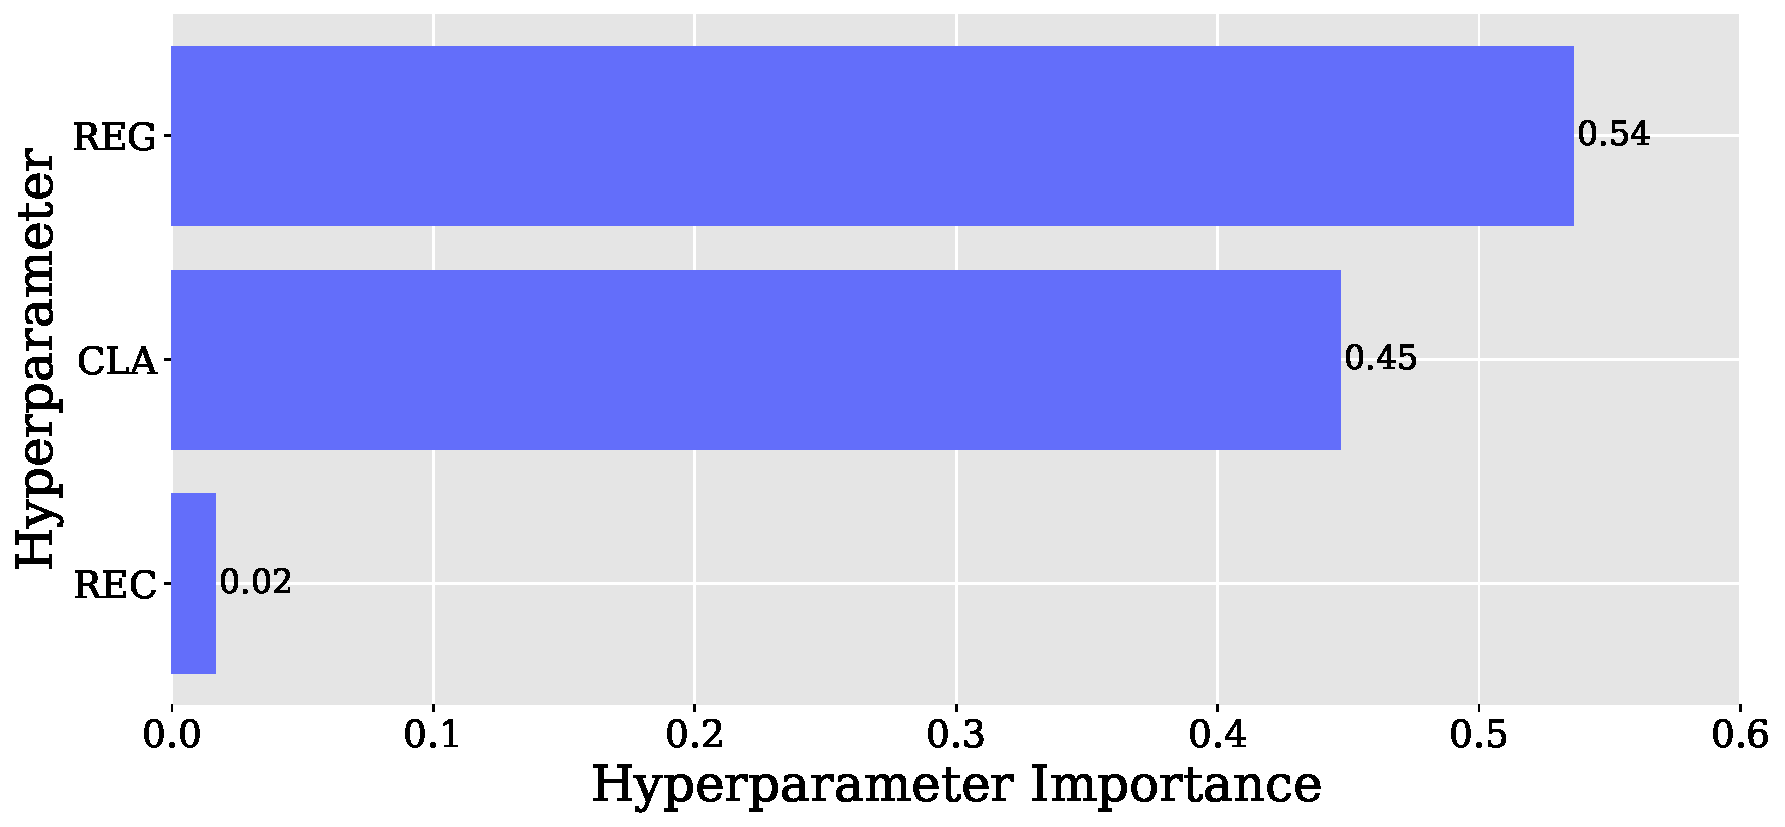
\includegraphics[width=0.8\linewidth]{Figures/optuna_fanova_param_importances_PHY_NRVAE.pdf}
    \caption{{Global hyperparameter importance of the optimized \gls{eeggcirnet} loss weights on the \gls{eegmmidb} dataset. The importance scores quantify the relative contribution of reconstruction (REC), classification (CLA), and latent-space regularization (REG) weights to validation accuracy.}}
    \label{fig:eegmmidb_fanova_importance}
\end{figure}
%-------------------------------------------------------

{The global importance analysis in Figure~\ref{fig:eegmmidb_fanova_importance} shows that REG is the most influential loss-weight hyperparameter in the multi-class \gls{eegmmidb} scenario, with an importance score of $0.54$, followed closely by CLA ($0.45$), while REC shows a markedly lower global contribution ($0.02$). This result suggests that, when the decoding task involves multiple motor imagery and resting-state classes, validation performance is mainly shaped by the interaction between discriminative supervision and latent-space regularization. In this context, REG appears to play a central role in stabilizing the shared latent representation, while CLA remains essential for preserving class-specific separability. The low global importance of REC does not imply that reconstruction is irrelevant; rather, it indicates that its contribution is more subject-specific, as observed in cases such as Subject~41 and Subject~49. Overall, the \gls{eegmmidb} analysis confirms that \gls{eeggcirnet} adapts its optimization priorities according to task complexity, relying more strongly on latent-space regularization and classification guidance in the multi-class setting~\cite{lotte2018review,saha2020intra}.}

%-------------------------------------------------------
TDHA SGKF Under the subject-group validation scheme imposed by the SGKF-CV protocol, \gls{eeggcirnet} achieves a mean accuracy of $63.50\%$ across the five folds on the \gls{adhd}/control children dataset, as reported in Table~\ref{tab:tdha_eegcirnet_hps}. This moderate performance reflects the increased difficulty of the dataset and the strictness of group-wise validation, which prevents subject leakage between training and test partitions. Such a setting is particularly demanding in pediatric \gls{adhd} data, where inter-subject heterogeneity, attentional variability, and subject-dependent neural patterns complicate subject-independent generalization~\cite{lotte2018review,saha2020intra}.

%---------------------------------------------------
\begin{table}[H]
    \centering
    \caption{Bayesian-optimized loss weights and fold-wise accuracy of \gls{eeggcirnet} on the \gls{adhd}/control children dataset under SGKF validation.}
    \label{tab:tdha_eegcirnet_hps}
    \begin{tabularx}{\textwidth}{CCCCC}
        \toprule
        \textbf{Fold} & \textbf{REC} & \textbf{CLA} & \textbf{REG} & \textbf{ACC [\%]} \\
        \midrule
        1 & $0.4443$ & $0.1249$ & $0.4308$ & $66.49$ \\
        
        2 & $0.4802$ & $0.2194$ & $0.3004$ & $57.78$ \\
        
        3 & $0.1272$ & $0.4243$ & $0.4486$ & $63.02$ \\
        
        4 & $0.4501$ & $0.4368$ & $0.1130$ & $62.64$ \\
        
        5 & $0.3554$ & $0.4565$ & $0.1881$ & $67.56$ \\
        \midrule
        \textbf{Average} &  &  &  & $\mathbf{63.50}$ \\
        \bottomrule
    \end{tabularx}
\end{table}
%---------------------------------------------------

The optimized configurations reveal strong fold-wise variability in the allocation of REC, CLA, and REG. Since each SGKF fold contains a different held-out subject group, the fold-wise accuracy should not be interpreted as a direct consequence of a single loss-weight pattern. Instead, Table~\ref{tab:tdha_eegcirnet_hps} shows that \gls{eeggcirnet} adapts its optimization balance according to the specific train--test split. Fold~1 follows a REC--REG-oriented configuration, Fold~2 assigns its largest contribution to REC with additional REG support, Fold~3 shifts toward a CLA--REG strategy, whereas Folds~4 and~5 emphasize REC--CLA with lower REG. This variability indicates that no single loss-weight configuration is uniformly optimal across folds. Importantly, all three components remain active across folds, suggesting that reconstruction fidelity, discriminative supervision, and latent-space regularization jointly contribute to maintaining training stability under strict subject-independent validation.

{To further examine the optimization behavior under the SGKF-CV protocol, we analyzed the validation-accuracy landscape obtained from the hyperparameter search across the five folds. Unlike the previous contour analyses for GigaScience, BCI Competition IV-2a, and \gls{eegmmidb}, this analysis does not correspond to a representative subject, but rather to the global behavior induced by the fold-wise validation scheme. Therefore, the contour plots in Figure~\ref{fig:contour_tdha-EEGCIRNET} summarize how different combinations of the normalized reconstruction (REC), classification (CLA), and latent-space regularization (REG) weights affect validation accuracy across heterogeneous train--test subject splits in the \gls{adhd}/control children dataset.}

%----------------------------------------------------
\begin{figure}[H]
\centering

\makebox[\textwidth][c]{%
\begin{minipage}[c]{0.99\textwidth}
\centering

\subfloat[REC vs. CLA]{%
    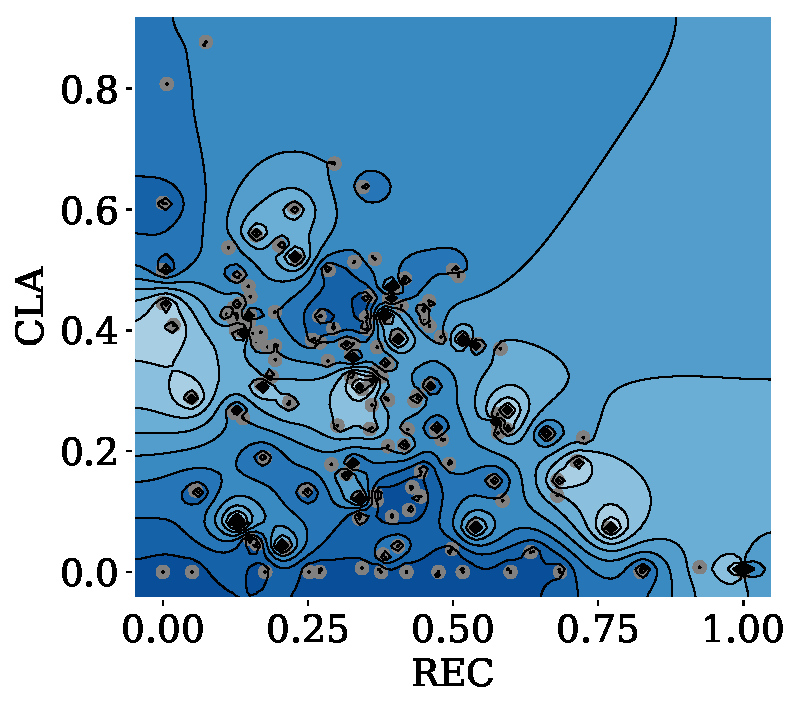
\includegraphics[width=0.34\linewidth,height=3.4cm]{Figures/contour_REC_vs_CLA-adhd.pdf}
}
\subfloat[REC vs. REG]{%
    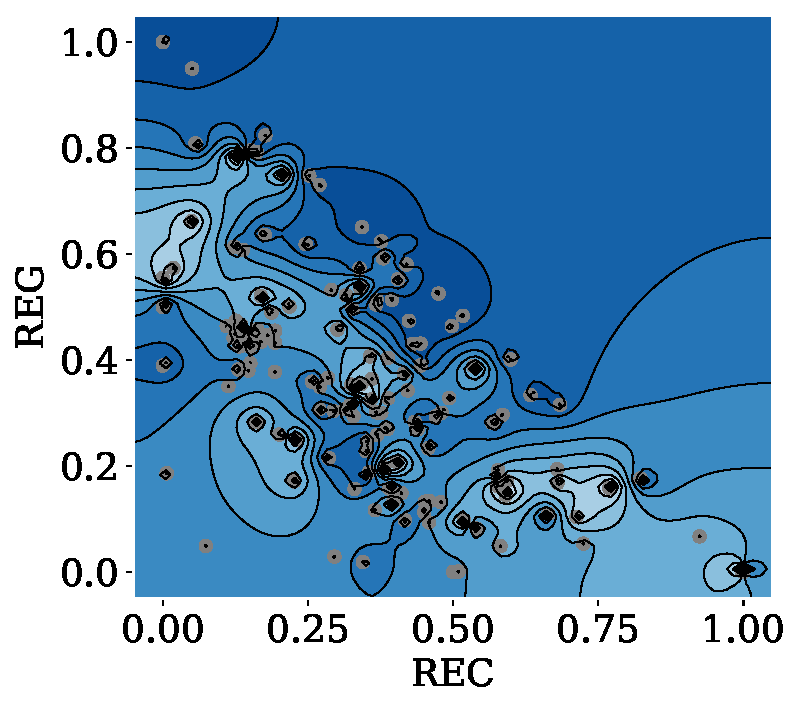
\includegraphics[width=0.34\linewidth,height=3.4cm]{Figures/contour_REC_vs_REG-adhd.pdf}
}
\subfloat[CLA vs. REG]{%
    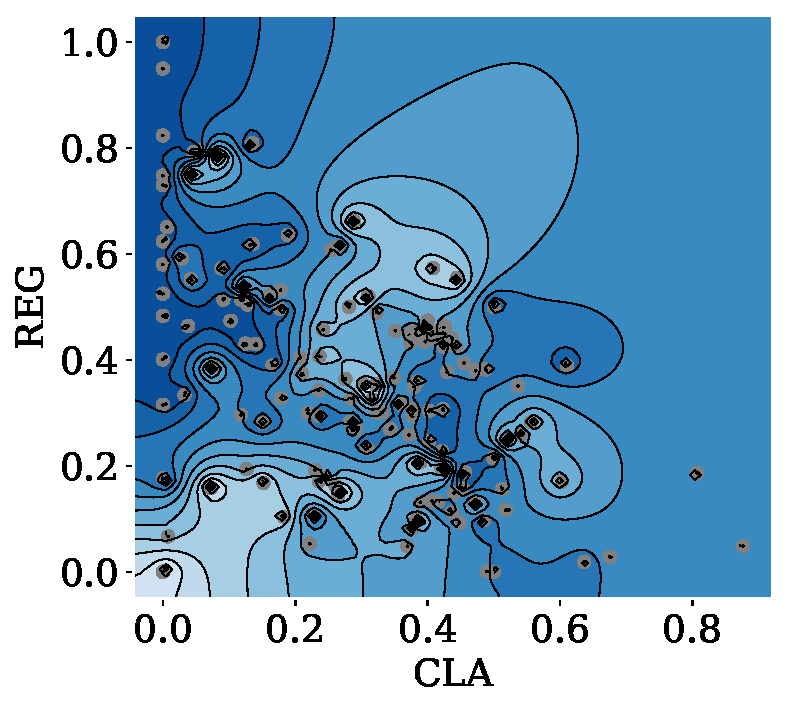
\includegraphics[width=0.34\linewidth,height=3.4cm]{Figures/contour_CLA_vs_REG-adhd.pdf}
}

\vspace{0.6em}

\begin{tikzpicture}
\begin{axis}[
    hide axis,
    scale only axis,
    width=\linewidth,
    height=0pt,
    colormap name=optunablues,
    colorbar horizontal,
    point meta min=42,
    point meta max=66,
    colorbar style={
        width=\linewidth,
        height=3mm,
        xtick={42, 46, 50, 54, 58, 62, 66},
        xticklabel style={font=\scriptsize},
        xlabel={Val. accuracy (\%)},
        xlabel style={font=\scriptsize, yshift=2pt},
        scaled ticks=false,
        /pgf/number format/fixed,
        /pgf/number format/precision=1,
    },
]
\addplot [draw=none] coordinates {(0,0)};
\end{axis}
\end{tikzpicture}

\end{minipage}%
}

\caption{{Contour plots of validation accuracy (\%) as a function of the normalized loss weights REC, CLA, and REG for the \gls{adhd}/control children dataset under the SGKF-CV validation scheme. All panels share the same color scale, allowing direct visual comparison across loss-weight pairs.}}
\label{fig:contour_tdha-EEGCIRNET}
\end{figure}
%----------------------------------------------------

{Figure~\ref{fig:contour_tdha-EEGCIRNET} reveals a highly irregular validation-accuracy landscape for the \gls{adhd}/control children dataset under the SGKF-CV protocol. Unlike the smoother and more structured patterns observed in the BCI-oriented datasets, the contour maps show multiple localized regions of varying performance rather than a single broad optimum. This behavior is particularly evident in the REC--CLA and CLA--REG projections, where regions of improved validation accuracy appear scattered across the loss-weight space, indicating that the model is highly sensitive to small changes in the relative contribution of reconstruction, classification, and latent-space regularization.}

{This fragmented landscape is consistent with the strict nature of SGKF-CV, where each fold evaluates the model on unseen subject groups. In this setting, subject-dependent neural patterns, inter-subject heterogeneity, and variability in the recorded responses can reduce class separability and increase the variability of the validation response~\cite{lotte2018review,saha2020intra,lenartowicz2018adhd}. Therefore, the absence of a single stable high-performance region suggests that \gls{eeggcirnet} must adapt its objective balance according to the particular train--test subject split.}

{Overall, the \gls{adhd}/control children dataset contour analysis supports the interpretation derived from Table~\ref{tab:tdha_eegcirnet_hps}: no fixed combination of REC, CLA, and REG is uniformly optimal across folds. Instead, \gls{eeggcirnet} benefits from dynamic multi-objective reweighting, where reconstruction fidelity, discriminative supervision, and latent-space regularization jointly contribute to maintaining stable learning under heterogeneous subject-group validation.}
%-------------------------------------------------------

{After analyzing the fold-wise contour maps, we performed a global hyperparameter-importance analysis to identify which loss component most strongly influenced validation accuracy under the SGKF-CV protocol. This analysis provides a complementary dataset-level view of the optimization behavior of \gls{eeggcirnet} on the \gls{adhd}/control children dataset.}

\begin{figure}[H]
    \centering
    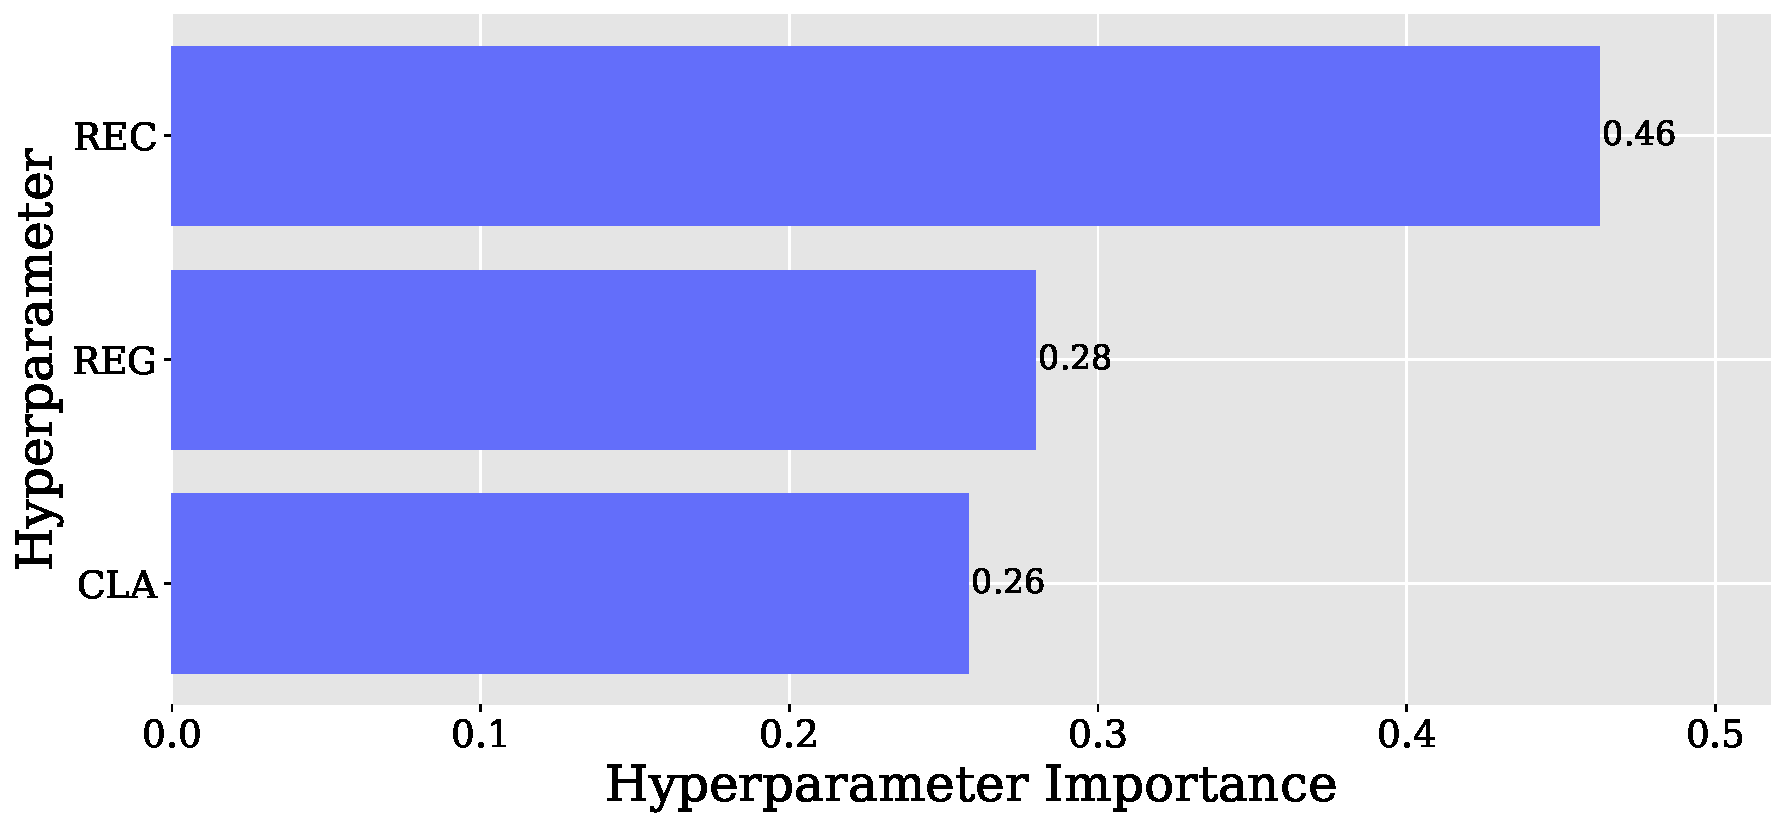
\includegraphics[width=0.8\linewidth]{Figures/optuna_fanova_param_importances_TDHA_NRVAE.pdf}
    \caption{{Global hyperparameter importance of the optimized \gls{eeggcirnet} loss weights on the \gls{adhd}/control children dataset under the SGKF-CV protocol. The importance scores quantify the relative contribution of reconstruction (REC), classification (CLA), and latent-space regularization (REG) weights to validation accuracy.}}
    \label{fig:TDHA_NRVAE}
\end{figure}
%----------------------------------------------------

{The global importance analysis in Figure~\ref{fig:TDHA_NRVAE} shows that REC is the most influential loss-weight hyperparameter in the \gls{adhd}/control children dataset, with an importance score of $0.46$, followed by REG ($0.28$) and CLA ($0.26$). This result indicates that, under strict subject-group validation, validation accuracy is primarily shaped by the model's ability to preserve and reconstruct stable connectivity-based representations. At the same time, the comparable contributions of REG and CLA suggest that latent-space stabilization and discriminative supervision remain necessary to support classification under heterogeneous train--test subject splits. Therefore, \gls{eeggcirnet} does not rely exclusively on the classification objective; instead, it benefits from a multi-objective balance in which reconstruction fidelity plays a central role while regularization and classification provide complementary support. This behavior is consistent with the known difficulty of subject-independent \gls{eeg} generalization under inter-subject variability and heterogeneous neural patterns~\cite{lotte2018review,saha2020intra,lenartowicz2018adhd}.}
%----------------------------------------------------

\subsubsection{Qualitative Analysis of Learned Representations and Functional Connectivity}

The adaptive weighting strategy of the proposed loss function directly influences the quality of the learned representations, which can be assessed by analyzing the decoder's output. Figures~\ref{fig:band14} and~\ref{fig:band27} present the class-specific topographic reconstructions for a representative ``Good'' subject (Subject $14$) and a ``Mid'' subject (Subject $27$). For Subject $14$, the reconstructions are spatially homogeneous, reflecting the ``Good'' group's balanced optimization where the model maintains a stable, regularized latent space. Conversely, for Subject $27$, the reconstructions appear sharper and more structurally defined. This aligns perfectly with the ``Mid'' group's adaptive increase in the reconstruction weight ($\lambda_{\text{REC}}$), which forces the model to prioritize structural fidelity to capture the more complex or noisy signal distributions inherent to this group. The ability to generate coherent and class-consistent topographic maps demonstrates that the VAE successfully captures relevant spatio-spectral patterns.

To validate that these reconstructed topographies represent genuine neural interactions rather than artifacts, we analyzed the underlying functional connectivity networks. Figure~\ref{fig:connectivities} illustrates the average connectivity patterns for the same representative subjects ($14$ and $27$), organized by anatomical region and hemisphere. The edges represent the strongest functional connections ($95$-th to $100$-th percentile), revealing distinct network topologies associated with performance levels.

\begin{figure}[H]
    \centering
    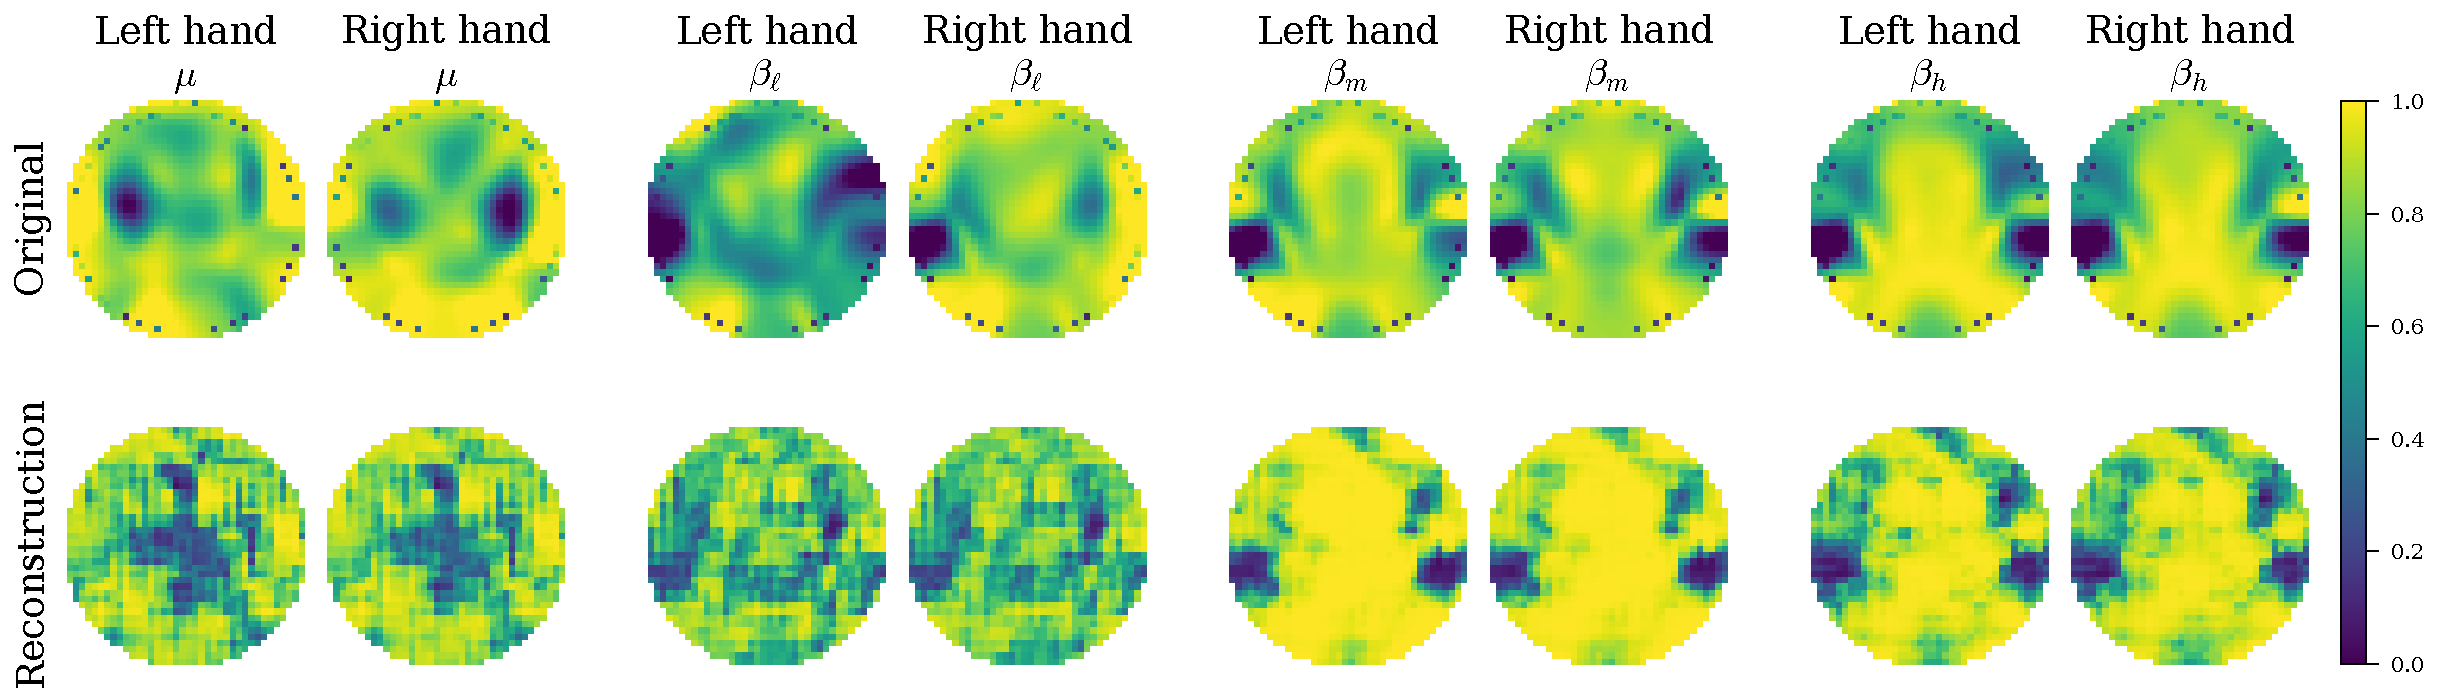
\includegraphics[width=1\linewidth]{Figures/topomaps_bands_14.pdf}
    \caption{Reconstruction subject 14 corresponding to group ``Good''.}
    \label{fig:band14}
\end{figure}
\vspace{-10pt}
\begin{figure}[H]
    \centering
    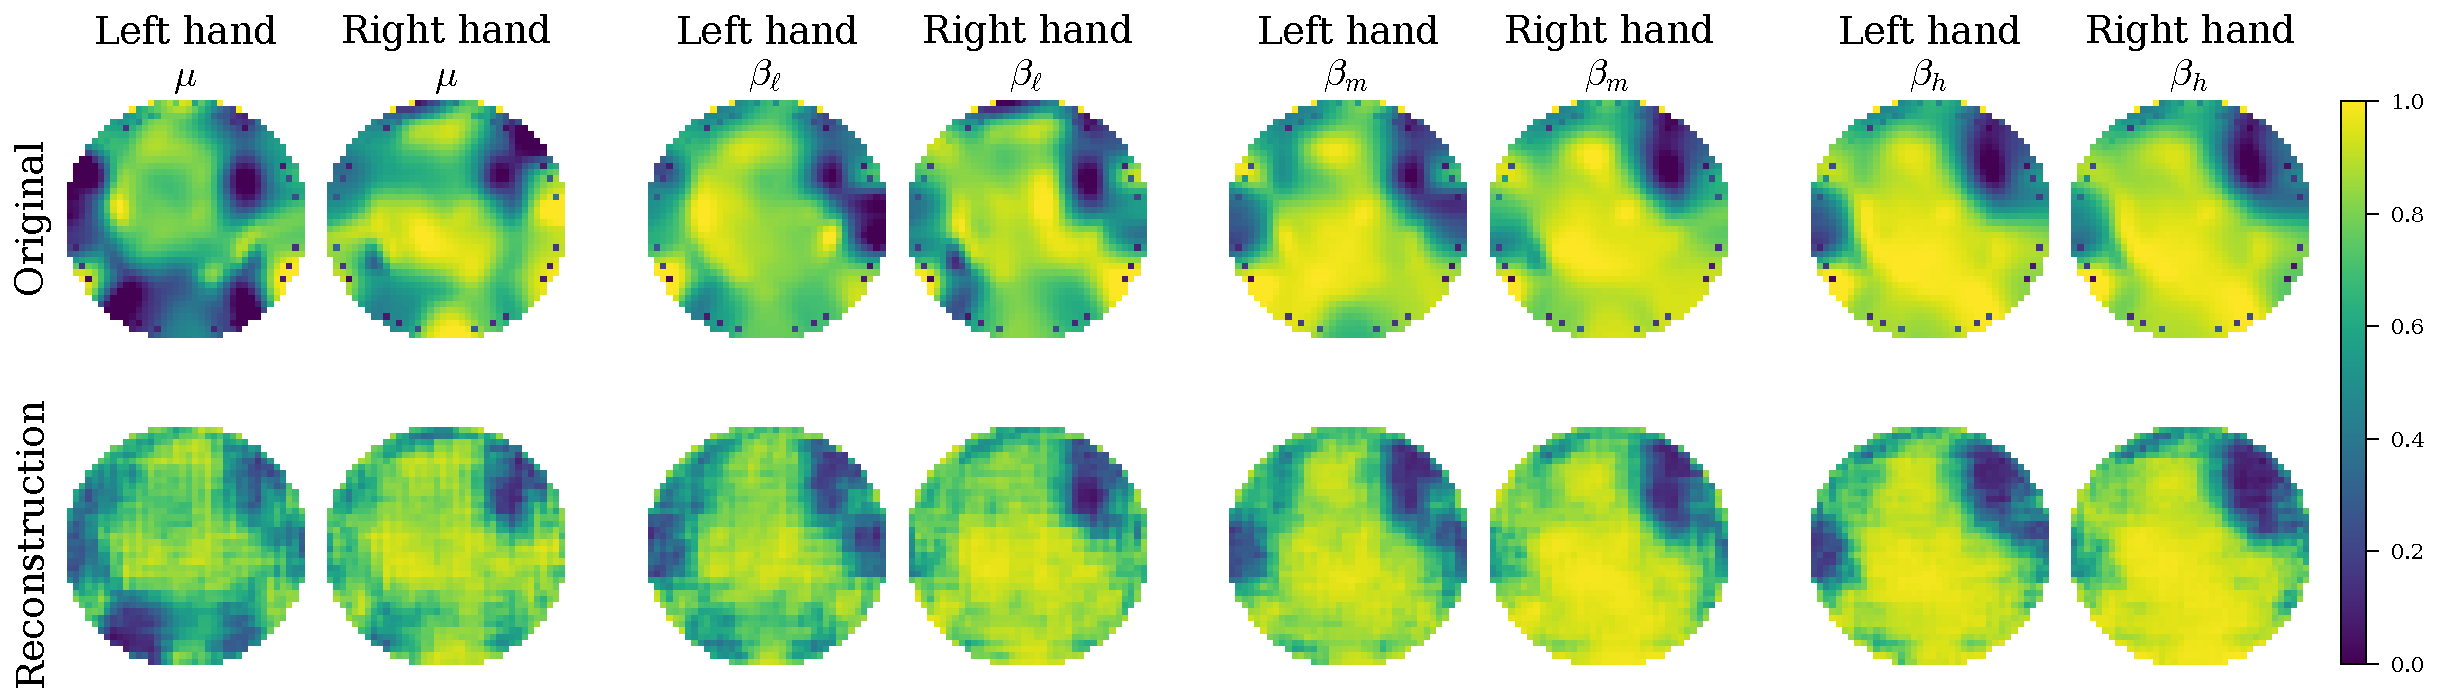
\includegraphics[width=1\linewidth]{Figures/topomaps_bands_27.pdf}
    \caption{Reconstruction subject 27 representing group ``Mid''.}
    \label{fig:band27}
\end{figure}

In the case of the high-performing Subject $14$, the connectivity patterns reveal a highly integrated network. In the $\mu$ band, relevant connections link frontal regions to the right central area, and from there to posterior regions (e.g., P2 to Pz), suggesting a cohesive fronto-centro-parietal network. As the frequency increases into the $\beta$ bands ($\beta_l$, $\beta_m$, $\beta_h$), this integration intensifies. We observe consistent inter-hemispheric links among posterior regions and salient connections bridging midline and left frontal regions (e.g., Fz--F1). This coordinated involvement of bilateral frontal cortices and the sustained posterior coupling supports the notion that high performance is driven by robust long-range synchronization.

In contrast, the connectivity profile of the mid-performing Subject $27$ indicates a different neural strategy, necessitating the model's enhanced focus on reconstruction. Across the $\mu$ and low-$\beta$ bands, connections are heavily concentrated along the central and centro-parietal midline (particularly C1--Cz and CP1--CPz), with a prominent additional link emerging between Pz and P1. Unlike the broad integration seen in the good performer, this subject exhibits a redistribution of connectivity toward fronto-central and centro-posterior networks. In the mid- and high-$\beta$ bands, this configuration remains stable, highlighting a sustained involvement of left posterior parietal regions.
%-----------------------------------------------
\begin{figure}[H]
         \subfloat[Subject 14 group good]{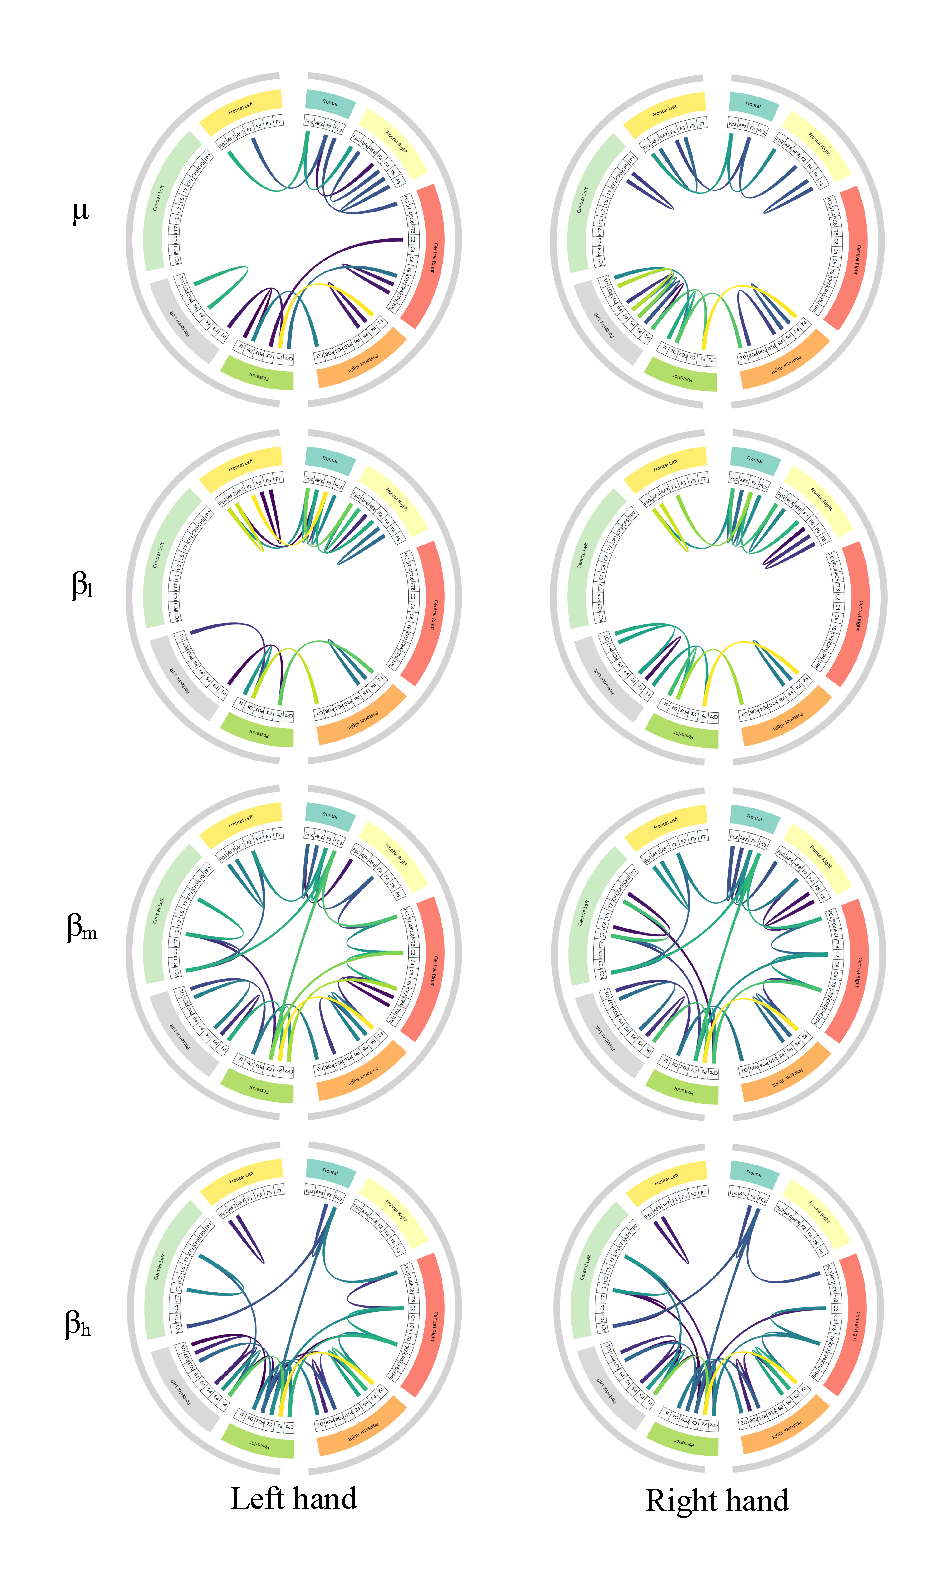
\includegraphics[height=11cm]{Figures/14.pdf}}
         \label{fig:14}
         \subfloat[Subject 27 group mid]{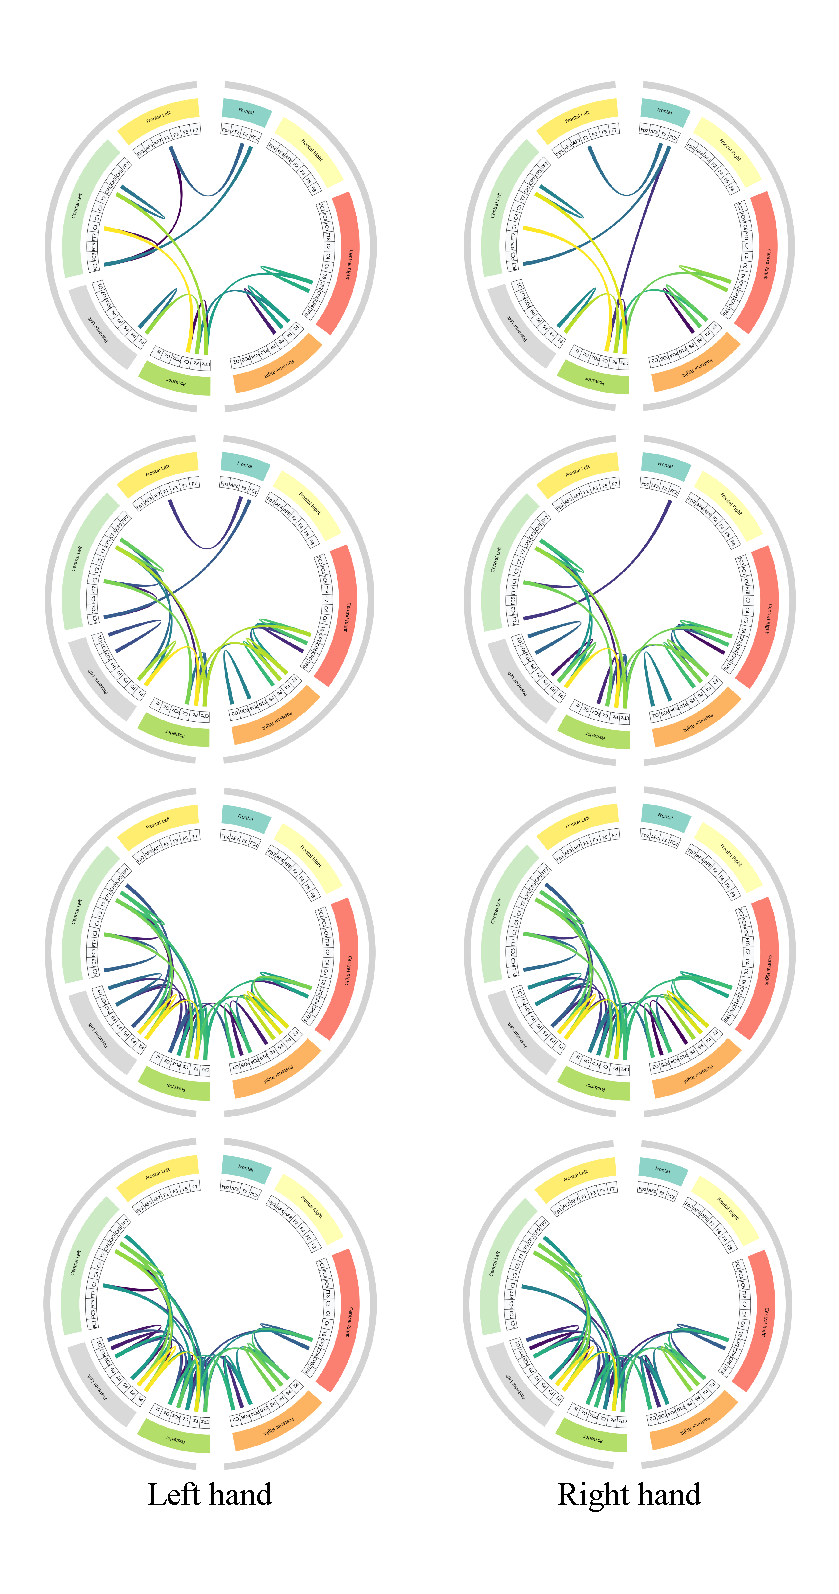
\includegraphics[height=11cm]{Figures/27.pdf}}
         \label{fig:27}
    \vspace{0.4em}
    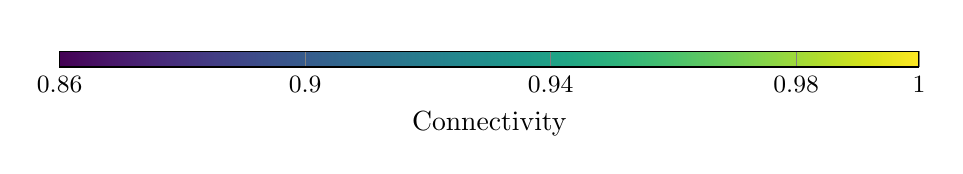
\begin{tikzpicture}
      \begin{axis}[
        hide axis,
        scale only axis,
        height=0,
        width=0.9\textwidth,
        colormap/viridis,
        colorbar horizontal,
        point meta min=0.86,
        point meta max=1.0,
        colorbar style={
          width=0.9\linewidth,
          height=2mm,
          xlabel={Connectivity},
          xtick={0.86,0.90,0.94,0.98,1.00},
          xticklabel style={font=\small},
        },
      ]
        \addplot [draw=none] coordinates {(0,0) (1,1)};
      \end{axis}
    \end{tikzpicture}

    \caption{Functional connectivity patterns for two representative subjects. For each subject, the left and right columns correspond to left- and right-hand \gls{mi}, respectively, and the rows correspond to the  $\mu$, $\beta_l$, $\beta_m$, and $\beta_h$ bands.}
    \label{fig:connectivities}
\end{figure}
%-----------------------------------------------

The persistence of these specific frequency-dependent connections over sensorimotor and parietal areas in both subjects confirms that the reconstructed maps are biologically valid. The model effectively captures the integrated fronto-parietal networks typical of high performers, as well as the more localized, midline-focused compensatory networks of mid performers. This demonstrates that the \gls{eeggcirnet} does not simply memorize input images, but learns to encode and reconstruct the underlying physiological connectivity drivers of \gls{mi}.

\subsubsection{Structure and Separability of the Latent Space}

The ultimate outcome of the model's adaptive learning and representation quality is a well-structured and discriminative latent space. To visualize this, t-SNE projections were applied to the latent representations of subjects $14$ and $27$ (Figure~\ref{fig:tsne}).

For the high-performing subject $14$ (Figure~\ref{fig:tsne}a), the projection reveals two clearly differentiated and cohesive clusters corresponding to the left- and right-hand MI classes. This well-defined separation confirms that the model has learned a highly discriminative latent space, which is consistent with the subject's high classification accuracy. For the mid-performing subject $27$ (Figure~\ref{fig:tsne}b), the classes are still largely separable, though with some regions of overlap. This is typical for signals with lower quality, where features are partially discriminative but affected by noise~\cite{lee2022intertask, ng2023unsupervised, mishra2024adversarial}.

%------------------------------------------------
\begin{figure}[htbp]
         \subfloat[Subject 14 group good]{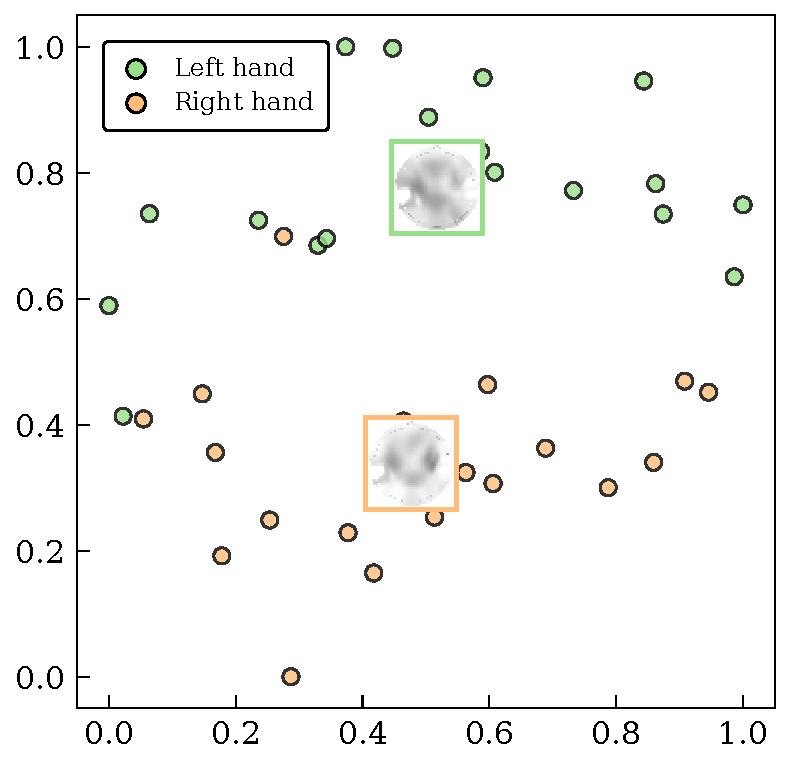
\includegraphics[height=6.5cm]{Figures/t-SNE-14-NRVAE.pdf}}
         \label{fig:tsene14_NRVAE}
     \hfill
     \subfloat[Subject 27 group mid]{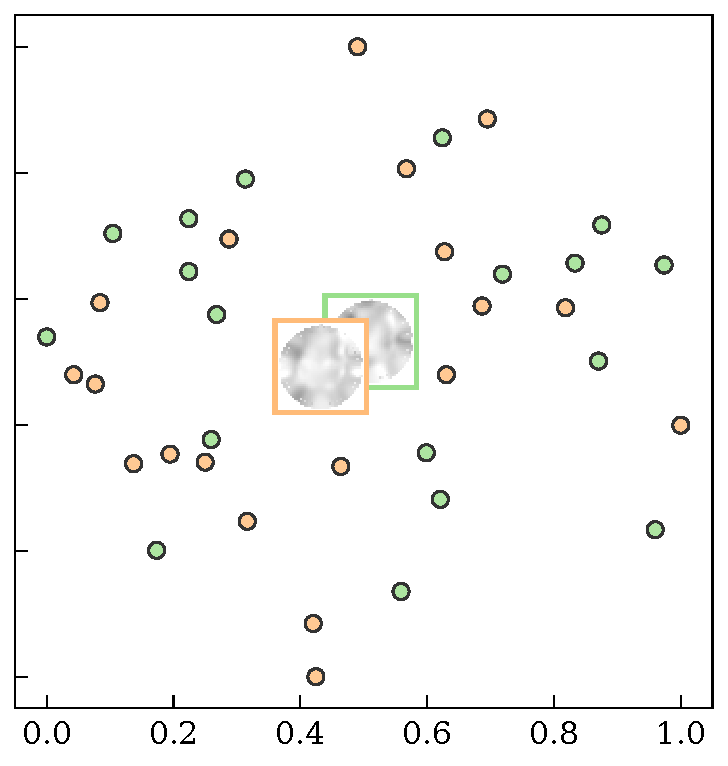
\includegraphics[height=6.5cm]{Figures/t-SNE-27-NRVAE.pdf}}
         \label{fig:tsne27_NRVAE}
    \caption{t-SNE of latent representations by performance group, good and mid. Colors correspond to the \gls{mi} classes (left hand and right hand).}
    \label{fig:tsne}
\end{figure}
%------------------------------------------------

Taken together, these visualizations confirm that \gls{eeggcirnet}'s VAE-based design successfully creates a more structured and discriminative latent space than is typically achievable with standard architectures. This underscores the critical role of latent space regularization in adapting to inter-subject variability and improving generalization, even in the presence of noisy inputs~\cite{ahmed2022latent, sharma2023review}.

\subsubsection{Layer-Wise Relevance Analysis via Grad-CAM++}

{Figure~\ref{fig:cams_subjects} displays the Grad-CAM++ relevance maps in the channel--subject plane for each of the three convolutional layers of the proposed architecture (\texttt{conv1}, \texttt{conv2}, and \texttt{conv3}) and for both MI classes. Unlike aggregate measures, this visualization presents the CAM corresponding to the model trained on that specific subject separately for each layer and class. It is important to note that these maps do not represent static filter weights; rather, they quantify the spatial contribution of each electrode to the model's decision, computed via the gradient-weighted combination of feature maps.}


{In the first convolutional layer (\texttt{conv1}), both classes exhibit broadly distributed activations across subjects and channels, indicating that this layer primarily captures generic spatio-spectral patterns. As the data propagates to \texttt{conv2}, the contribution becomes noticeably more focal, exhibiting clearly delineated channel-wise regions that depend on the MI class. This shift suggests that the model begins to combine spatial and channel information in a more specific manner. Finally, in the deepest layer (\texttt{conv3}), the CAMs become highly sparse and localized, concentrating on a small subset of subjects and channels. This behavior is consistent with a higher degree of specialization, where the deepest layer extracts highly discriminative features directly linked to the final MI decision.}

{Importantly, the CAM amplitudes are not trivially explained by the classification accuracy of each subject. Some subjects with high MI performance still show relatively diffuse or low-amplitude CAMs, whereas others with lower performance may exhibit more pronounced, localized patterns. This indicates that Grad-CAM++ is highlighting how each subject-specific model internally assigns importance to channels to solve the MI task, rather than simply mirroring inter-subject performance differences. Nevertheless, despite training a separate model per subject, the importance maps reveal consistent horizontal bands across subjects, pointing to a degree of cross-subject convergence in the channels that the network considers informative for left- and right-hand MI.}\\


\newlength{\camswidth}
\begin{figure}[H]
  
  \setlength{\camswidth}{0.44\textwidth}% ancho de cada subfigura

  \hspace*{-2em}%
  \makebox[\textwidth]{%
    % ==== Columna izquierda: etiqueta vertical "Channels" ====
    \begin{minipage}[c]{0.18\textwidth}
      \centering
      \rotatebox{90}{\normalsize Channels}
    \end{minipage}%
    \hspace{-1em}% ajusta este espacio si quieres acercar/alejar

    % ==== Columna derecha: las 6 subfiguras + colorbar ====
    \begin{minipage}[c]{0.90\textwidth}
      \centering
      \vspace{4pt}

      % ===== Fila 1 =====
      \subfloat[conv1 -- Left]{%
        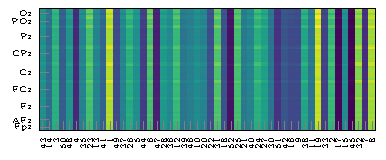
\includegraphics[width=\camswidth]{Figures/Conv1_Left.pdf}%
      }\hspace{0.3em}%
      \subfloat[conv1 -- Right]{%
        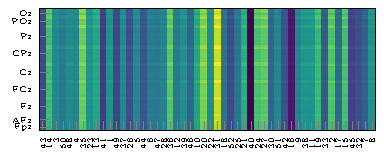
\includegraphics[width=\camswidth]{Figures/Conv1_Right.pdf}%
      }\\[0.5em]

      % ===== Fila 2 =====
      \subfloat[conv2 -- Left]{%
        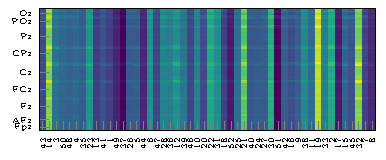
\includegraphics[width=\camswidth]{Figures/Conv2_Left.pdf}%
      }\hspace{0.3em}%
      \subfloat[conv2 -- Right]{%
        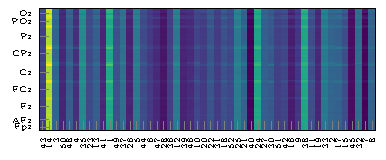
\includegraphics[width=\camswidth]{Figures/Conv2_Right.pdf}%
      }\\[0.5em]

      % ===== Fila 3 =====
      \subfloat[conv3 -- Left]{%
        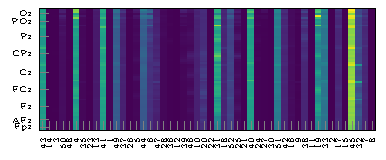
\includegraphics[width=\camswidth]{Figures/Conv3_Left.pdf}%
      }\hspace{0.3em}%
      \subfloat[conv3 -- Right]{%
        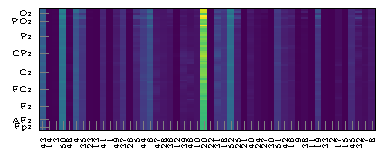
\includegraphics[width=\camswidth]{Figures/Conv3_Right.pdf}%
      }\\[0.8em]

      % ===== Barra de color compartida (creada en TikZ) =====
      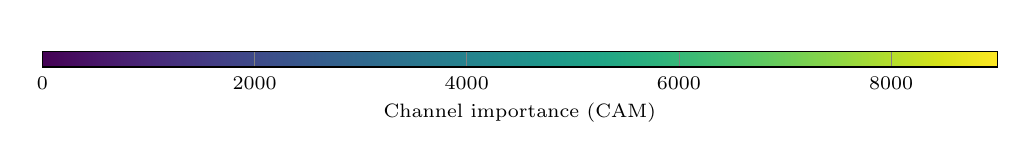
\begin{tikzpicture}
        \begin{axis}[
          hide axis,
          scale only axis,
          width=0.9\textwidth,   % largo de la barra
          height=0pt,
          colormap/viridis,
          colorbar,
          colorbar horizontal,
          point meta min=0,
          point meta max=9000, 
          colorbar style={
          width=1\linewidth,
          height=2mm,
          xtick={0,2000,4000,6000,8000},
          xticklabel style={
          font=\scriptsize,
          /pgf/number format/1000 sep={} % ← sin comas en 2,000 → 2000
          },
          xlabel={Channel importance (CAM)},
          xlabel style={font=\scriptsize, yshift=2pt},
          scaled ticks=false,
          /pgf/number format/fixed,
          /pgf/number format/precision=0,
          },
        ]
          % Plot fantasma solo para que pgfplots dibuje la barra
          \addplot[draw=none] coordinates {(0,0)};
        \end{axis}
      \end{tikzpicture}

    \end{minipage}% 
  }
  \caption{Channel-wise CAM contribution across subjects for each convolutional layer and MI class. The color intensity represents the relative importance of each channel in the model's decision-\mbox{making process}.}
  \label{fig:cams_subjects}
\end{figure}

To assess whether the interpretability of the learned features holds in the more complex multi-class scenario, we extended the Grad-CAM++ analysis to the \gls{eegmmidb} dataset. Figure~\ref{fig:cams_subjects1} depicts the relevance maps for four representative classes (C1--C4) across the network depth. Consistent with the binary classification findings, the network exhibits a clear hierarchical refinement of spatial contribution. 


% =========================================================
% =========================================================
% FIGURE: Channel-wise CAMs (solo MI C1--C4, compacta)
% =========================================================
\begin{figure}[H]


% ---------- Dimensiones ----------
\setlength{\camswidth}{0.215\textwidth} % 4 columnas

\newlength{\camsheight}
\setlength{\camsheight}{2.0cm}

\makebox[\textwidth][c]{%

% ================= ETIQUETA VERTICAL =================
\begin{minipage}[c]{0.035\textwidth}
  \centering
  \rotatebox{90}{\normalsize Channels}
\end{minipage}%
\hspace{0.6em}

% ================= MATRIZ 3 × 4 =================
\begin{minipage}[c]{0.94\textwidth}
\centering

% ================= FILA 1 : conv1 =================
\subfloat[conv1--C1]{%
  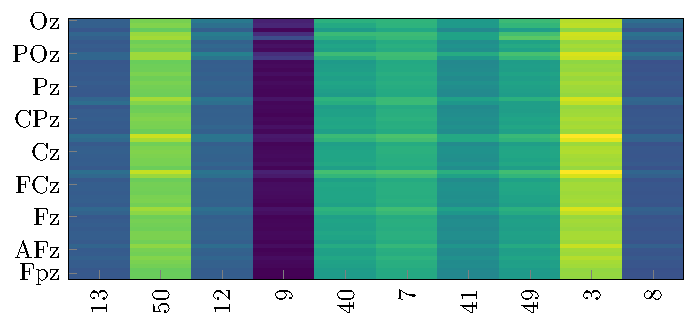
\includegraphics[width=\camswidth,height=\camsheight]{Figures/Conv1 Class1.pdf}} \hfill
\subfloat[conv1--C2]{%
  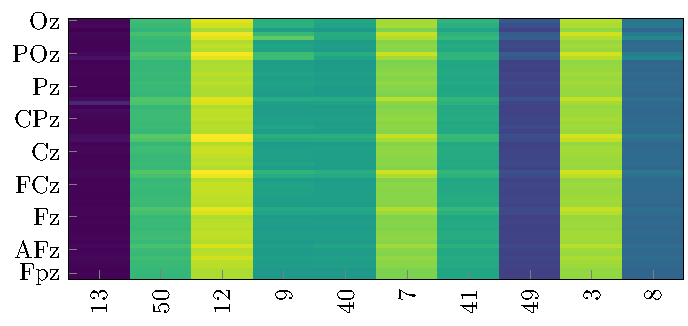
\includegraphics[width=\camswidth,height=\camsheight]{Figures/Conv1 Class2.pdf}} \hfill
\subfloat[conv1--C3]{%
  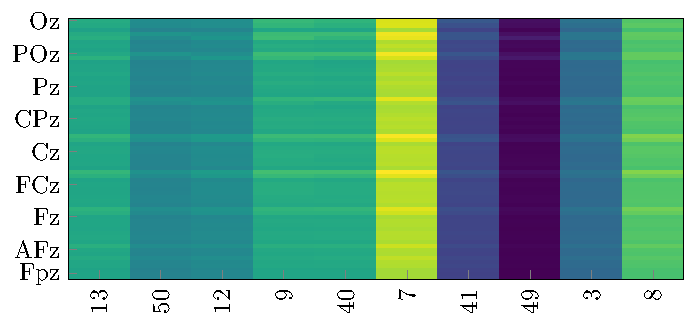
\includegraphics[width=\camswidth,height=\camsheight]{Figures/Conv1 Class3.pdf}} \hfill
\subfloat[conv1--C4]{%
  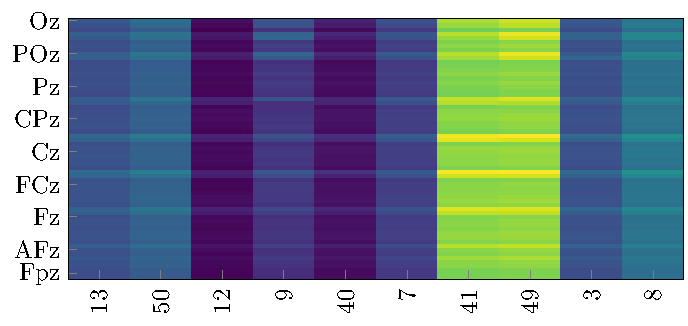
\includegraphics[width=\camswidth,height=\camsheight]{Figures/Conv1 Class4.pdf}} \\[0.3em]

% ================= FILA 2 : conv2 =================
\subfloat[conv2--C1]{%
  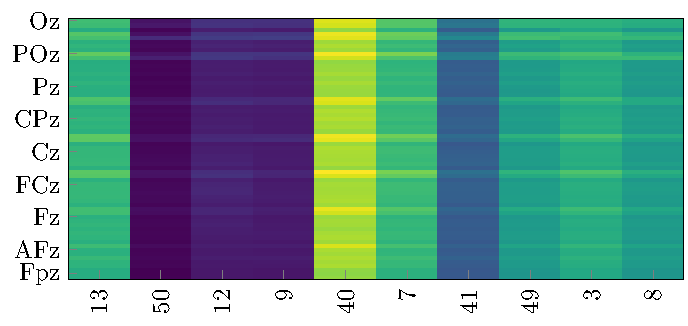
\includegraphics[width=\camswidth,height=\camsheight]{Figures/Conv2 Class1.pdf}} \hfill
\subfloat[conv2--C2]{%
  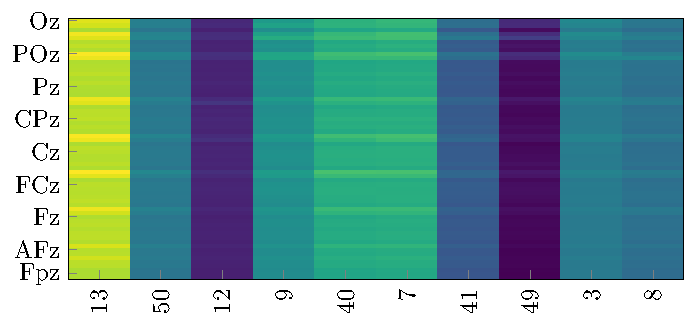
\includegraphics[width=\camswidth,height=\camsheight]{Figures/Conv2 Class2.pdf}} \hfill
\subfloat[conv2--C3]{%
  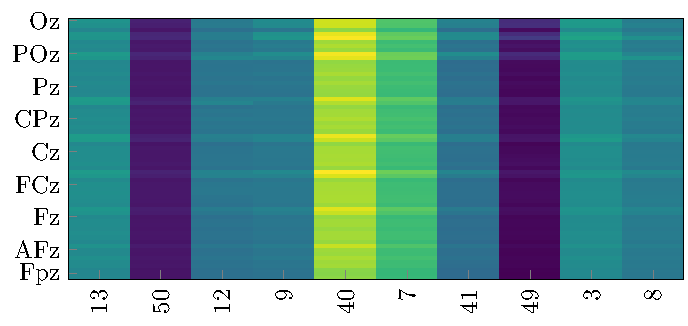
\includegraphics[width=\camswidth,height=\camsheight]{Figures/Conv2 Class3.pdf}} \hfill
\subfloat[conv2--C4]{%
  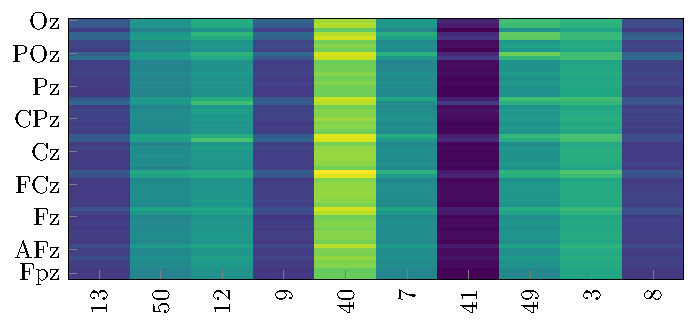
\includegraphics[width=\camswidth,height=\camsheight]{Figures/Conv2 Class4.pdf}} \\[0.3em]

% ================= FILA 3 : conv3 =================
\subfloat[conv3--C1]{%
  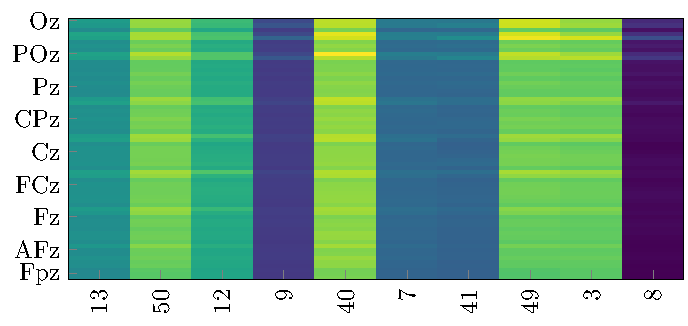
\includegraphics[width=\camswidth,height=\camsheight]{Figures/Conv3 Class1.pdf}} \hfill
\subfloat[conv3--C2]{%
  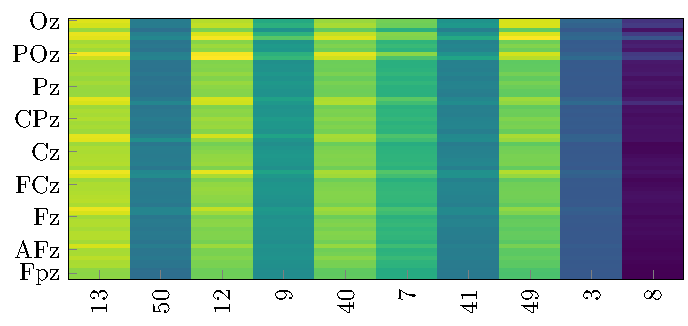
\includegraphics[width=\camswidth,height=\camsheight]{Figures/Conv3 Class2.pdf}} \hfill
\subfloat[conv3--C3]{%
  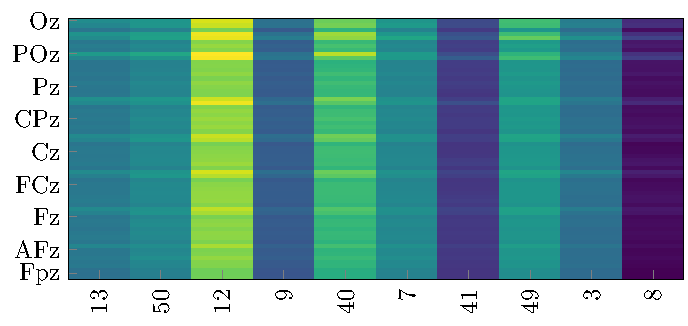
\includegraphics[width=\camswidth,height=\camsheight]{Figures/Conv3 Class3.pdf}} \hfill
\subfloat[conv3--C4]{%
  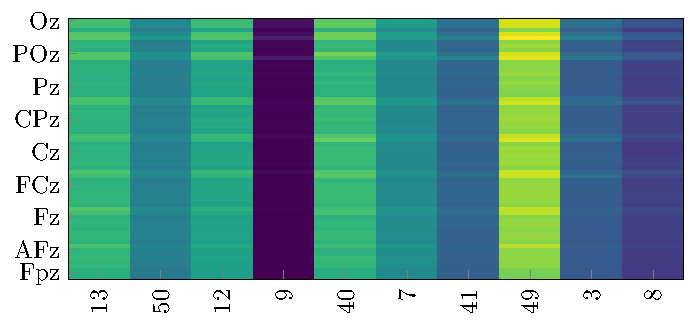
\includegraphics[width=\camswidth,height=\camsheight]{Figures/Conv3 Class4.pdf}} \\[0.7em]

% ================= COLORBAR =================
\hspace{-6pt}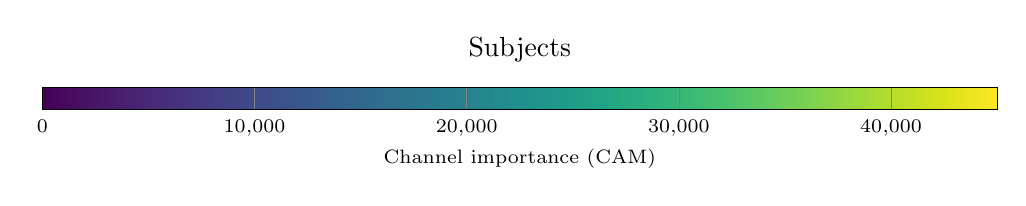
\begin{tikzpicture}
\begin{axis}[
  hide axis,
  scale only axis,
  width=0.99\textwidth,
  height=0pt,
  colormap/viridis,
  colorbar,
  colorbar horizontal,
  point meta min=0,
  point meta max=45000,
  colorbar style={
  width=1\linewidth,
  title={Subjects},
  height=2.8mm,
  xtick={0,10000,20000,30000,40000},
  xticklabel style={font=\scriptsize},
  xlabel={Channel importance (CAM)},
  xlabel style={font=\scriptsize, yshift=2pt},
  scaled ticks=false,
  /pgf/number format/fixed,
  /pgf/number format/precision=0,
},
]
\addplot[draw=none] coordinates {(0,0)};
\end{axis}
\end{tikzpicture}

\end{minipage}
}

% ================= CAPTION =================
\caption{Channel-wise class activation maps (CAMs) for \gls{mi} (MI) classes across convolutional layers.
Rows correspond to \textit{conv1}, \textit{conv2}, and \textit{conv3}, while columns (C1--C4) denote the selected MI classes.
Color intensity reflects the relative contribution of each \gls{eeg}channel, using a shared global color scale.}

\label{fig:cams_subjects1}
\end{figure}


In the initial layer (conv1, \mbox{Figure~\ref{fig:cams_subjects1}a--d}), the importance distribution is diffuse and spans vertically across nearly all channels for every class. This suggests that the shallow layers are primarily responsible for extracting low-level, generic spectral features shared among all motor tasks. However, as information flows to the deeper layers (conv3, \mbox{Figure~\ref{fig:cams_subjects1}}i--l), a high degree of spatial \mbox{specialization emerges}.

Notably, the multi-class scenario requires the model to resolve finer topological differences than simple hemispheric lateralization. The maps in the deepest layer (conv3) demonstrate that the model successfully learns distinct spatial signatures for each class. For instance, the channels contributing to Class 1 (Figure~\ref{fig:cams_subjects1}i) form a specific cluster that differs topographically from the channels driving the decision for Class 3 (Figure~\ref{fig:cams_subjects1}k). This spatial disentanglement confirms that \gls{eeggcirnet} solves the complex 5-class problem by isolating specific subsets of task-relevant electrodes—likely corresponding to the distinct cortical representations of hands and feet—rather than relying on global signal artifacts.

%------------------------------------------------
\subsection{Discussion}\label{sec:Discussion1}
%------------------------------------------------

The results obtained with the proposed \gls{eeggcirnet} architecture provide valuable insights into how model design and latent regularization can jointly address key challenges in \gls{mi} decoding. This study demonstrated that by transforming functional connectivity into an image-based representation and processing it with a variational autoencoder, it is possible to create a BCI framework that is not only highly accurate but also robust and interpretable. The model achieved remarkable performance across subjects, reaching the highest average accuracy ($81.82\%$) and the lowest inter-subject variability among all evaluated methods, confirming the efficacy of this unimodal, VAE-based approach.

{A key aspect of this contribution} lies in its direct response to the critical challenges of inter-subject variability and ``BCI illiteracy''. The most compelling finding was the complete elimination of the ``Bad'' performance group (Figure~\ref{fig:Violins}c), coupled with substantial accuracy gains of $21.55\%$ and $13.70\%$ for the ``Bad'' and ``Mid'' groups, respectively (Table~\ref{tab:accuracy_gain}). This demonstrates the profound robustness of \gls{eeggcirnet} in handling noisy or low-separability \gls{eeg} signals, where conventional architectures typically fail. By elevating the performance of these challenging subjects, the framework serves a corrective function, suggesting a promising path toward more inclusive and reliable BCI systems that can adapt to a wider range of users. {Furthermore, the scalability of the proposed framework is evidenced by its superior performance in the complex 5-class \gls{eegmmidb} scenario, where it achieved an average accuracy of $75.20\%$, surpassing advanced temporal-channel fusion models by approximately $6.3$\%. Unlike binary tasks, where hemispheric lateralization is often sufficient for discrimination, the 5-class problem requires the model to resolve finer topological differences between spatially overlapping classes, such as ``Both Hands'' versus single-hand imagery.

The mechanism underlying this robustness appears to be the model's sophisticated, adaptive learning strategy. The analysis of the loss weight distributions (Figure~\ref{fig:distributions}) revealed that \gls{eeggcirnet} is not a static ``black box'' but dynamically reorganizes its optimization priorities based on signal quality. In the bi-class scenario, for subjects with high-quality signals, it maintains a harmonious balance between reconstruction, classification, and regularization. For subjects with more challenging signals, it strategically prioritizes representation learning (REC loss) over immediate classification (CLA loss). This intelligent trade-off is visually confirmed by the qualitative analysis of the reconstructions (Figures~\ref{fig:band14} and~\ref{fig:band27}), which shows that the model consistently generates spatially coherent and physiologically plausible connectivity maps. This behavior supports the notion that a well-regularized and accurately reconstructed representation is a prerequisite for effective classification, especially in noisy conditions. {Moreover, as observed in Table~\ref{tab:weights_dist}, for the most challenging subjects (e.g., Subject 49) in multi-class scenario, the network implicitly shifts its role from a classifier to a non-linear denoiser ($\lambda_{\text{REC}} \approx 0.83$), prioritizing the reconstruction of a clean latent representation before attempting to separate complex decision boundaries. This suggests that the connectivity-driven topographic maps provide a sufficiently rich feature space to support multi-class decoding, provided that the training objective is dynamically regularized to handle the increased cognitive load and signal ambiguity.

The above is further corroborated by the functional connectivity analysis, which reveals distinct network topologies associated with performance levels (see Figure~\ref{fig:connectivities}). For high-performing subjects, the observed integrated fronto--centro--parietal network supports established findings on the critical role of fronto--parietal and parieto--occipital connectivity in supporting MI performance~\cite{Hamedi2016MIBrainConnectivityReview}, while the specific beta-band synchronization over central and parietal regions aligns with literature identifying these features as informative markers for task discrimination~\cite{cardoso2021pedalingMI}. Conversely, the connectivity profile of mid-performing subjects suggests a redistribution toward fronto--central and centro--posterior networks; notably, the persistence of $\mu/\beta$-band connections over sensorimotor and parietal areas in these subjects remains consistent with studies highlighting the fundamental role of these networks in effective BCI control~\cite{CaicedoAcosta2021DeepNeuralRegression,Vidaurre2020SensorimotorFC}.

The ultimate outcome of this adaptive process is the creation of a well-structured and discriminative latent space. The t-SNE visualizations (Figure~\ref{fig:tsne}) provide direct evidence that the encoder successfully learns to disentangle the features of different MI classes, creating clearly separated clusters for high-performing subjects and maintaining reasonable separation even for mid-performing subjects. This demonstrates that the variational formulation and structured latent regularization are the primary drivers of the model's superior performance, allowing it to move beyond the limitations of conventional architectures that often struggle with noisy or overlapping feature distributions.

To verify that these learned latent structures correspond to genuine neural mechanisms rather than artifacts, we examined the spatial contribution patterns identified by the network. The layer-wise analysis of the relevance maps reveals consistent spatial structures that align with anatomically meaningful channel groups (see Figure~\ref{fig:cams_subjects} and~\ref{fig:cams_subjects1}). High-contribution areas in the superior frontal region likely reflect higher-order cognitive control and attentional processes facilitating MI, consistent with reports of prefrontal involvement linked to imagery quality ~\cite{hetu2013neural,delange2008cortex,kurkin2023tmsdlpfc}. Meanwhile, prominent bands of importance spanning fronto-central and parietal sites correspond to the well-known fronto-parietal MI network—encompassing premotor and parietal regions recruited during kinesthetic and visual MI ~\cite{mustile2024walking} and align with established evidence of alpha and beta modulation and information flow across these regions~\cite{zhou2025vmi}. Thus, the specific emphasis on parieto-occipital electrodes in the deepest layers suggests the network leverages visuo-spatial components alongside sensorimotor rhythms, a view supported by studies indicating occipital recruitment and connectivity during visual-\gls{mi}~\cite{dijkstra2024evc}. Regarding the multi-class scenario, the extended Grad-CAM++ analysis confirms that \gls{eeggcirnet} addresses this complexity through hierarchical spatial refinement, evolving from generic spectral features in shallow layers to highly specialized, class-specific electrode clusters in deep layers. This capability is underpinned by the model's adaptive optimization strategy, which becomes even more pronounced in this high-complexity setting. Overall, these results confirm that the proposed architecture converges towards neurophysiologically plausible channel patterns, emphasizing networks repeatedly implicated in motor simulation.

Finally, the statistical analysis confirms the performance advantage of \gls{eeggcirnet} across different levels of task complexity. While the model secured a leading average ranking of $2.32$ ($p=0.007$) in the binary scenario (Table~\ref{tab:p-values_updated}), its dominance became even more pronounced in the multi-class evaluation (Table \ref{tab:p-values_updated1}). In this challenging 5-class setting, \gls{eeggcirnet} achieved a perfect average ranking of ${1.00}$ and a highly significant average Wilcoxon $p$-value of ${0.002}$, establishing a statistically clear superiority over advanced architectures like TCFusionNet and DeepConvNet. This indicates that the observed performance gains are not random fluctuations but a consistent outcome of the model’s design. By learning robust latent structures directly from connectivity-based topographic representations, \gls{eeggcirnet} emerges as a reliable, interpretable, and computationally efficient framework for \gls{mi} decoding. It effectively balances accuracy, generalization, and representational stability, allowing it to adapt to diverse subject profiles and maintain strong performance across varying signal quality conditions while preserving a physiologically consistent representational organization.

%------------------------------------------------
\subsection{Summary}\label{sec:Conclusions1}
%------------------------------------------------
In this chapter, we proposed \gls{eeggcirnet}, a novel unimodal framework based on a variational autoencoder, designed to process topographic representations of functional connectivity for \gls{mi} classification. Through an extensive experimental evaluation, we demonstrated that this approach effectively addresses several persistent challenges in \gls{eeg}-based \glspl{bci}, including low spatial resolution, susceptibility to noise, and inter-subject variability. By integrating Gaussian functional connectivity with a generative VAE architecture, the proposed framework produces spatially structured representations that enable simultaneous classification and reconstruction, providing both competitive performance and interpretability grounded in neurophysiology.

{Overall, the proposed framework demonstrates that} connectivity-driven representations can substantially enhance robustness and subject-level fairness in \gls{mi} decoding. On the binary GigaScience benchmark, \gls{eeggcirnet} achieved the highest average accuracy ($81.82\%$) and the lowest inter-subject variability ($\pm10.15$) among all evaluated baselines. Most notably, the model completely eliminated the ``Bad'' performance group (subjects with $<60\%$ accuracy) and yielded performance gains of approximately $22\%$ for these challenging users. This result, which is statistically significant ($p=0.007$), indicates that the variational formulation enables the extraction of discriminative information even from noisy or low-separability signals. Moreover, in the more complex 5-class \gls{eegmmidb} scenario, \gls{eeggcirnet} achieved a perfect average ranking of ${1.00}$ and a highly significant Wilcoxon $p$-value of ${0.002}$, confirming its scalability to multi-class decoding with overlapping spatial patterns.

Importantly, the generalization capability of the proposed framework was further validated on the BCI Competition IV-2a dataset, a widely standardized and subject-independent benchmark. Subject-wise analyses revealed that \gls{eeggcirnet} consistently outperformed EEGNet across all subjects, with the largest performance gains observed for individuals exhibiting lower baseline accuracies. This behavior highlights the robustness of the connectivity-driven representation to inter-subject variability and demonstrates that physiologically informed feature construction can rival the performance of substantially heavier architectures without increasing model complexity.

The strong empirical performance of \gls{eeggcirnet} is supported by its adaptive optimization behavior. Analysis of the loss component weights revealed that the model dynamically reorganizes its learning priorities based on signal quality. For high-performing subjects, reconstruction, classification, and regularization losses remain balanced, whereas for weaker subjects or high-complexity tasks, the model prioritizes representation learning. This adaptive trade-off allows \gls{eeggcirnet} to function as a non-linear denoiser, resulting in a well-structured latent space where \gls{mi} classes are clearly disentangled, as evidenced by t-\mbox{SNE} visualizations.

Complementary interpretability analyses further confirmed the physiological relevance of the learned representations. Grad-CAM++ visualizations revealed a hierarchical learning process, progressing from generic spectral features in early layers to highly localized, task-relevant activations in sensorimotor and parieto-occipital regions. Functional connectivity analyses demonstrated that the model captures biologically meaningful networks, including long-range fronto--centro--parietal integration in high-performing subjects and compensatory, localized connectivity patterns in mid-performing individuals. These findings confirm that \gls{eeggcirnet} bases its decisions on genuine neurophysiological mechanisms rather than spurious correlations.

Despite these strengths, the limitations of the proposed framework become evident under clinically challenging generalization settings. When evaluated on the \gls{adhd}/control children dataset using a strict Subject-Group K-Fold Cross-Validation protocol, \gls{eeggcirnet} achieved stable but comparatively lower accuracy than several specialized baselines. This result highlights that, in pediatric clinical datasets, the dominant challenge shifts from class separability toward robust subject-to-subject transfer under pronounced neurophysiological heterogeneity. While \gls{eeggcirnet} exhibited consistent behavior across folds, the observed performance gap indicates that connectivity-driven representations alone may be insufficient to fully compensate for domain shifts arising from developmental variability, recording conditions, and individual neurocognitive profiles.

Overall, these findings delineate the operational scope of \gls{eeggcirnet}. The proposed framework is particularly effective for \gls{mi}-based \glspl{bci} and standardized decoding scenarios, where physiologically grounded connectivity representations can substantially reduce inter-subject disparities. However, its performance on the \gls{adhd}/control dataset underscores the need for additional mechanisms—such as domain adaptation, adaptive normalization, or hybrid architectures—to address the extreme variability encountered in clinical pediatric populations. These results provide both validation of the framework’s strengths and clear direction for future extensions aimed at improving subject-independent generalization in real-world clinical \gls{eeg} applications.
